\documentclass[twoside]{book}

% Packages required by doxygen
\usepackage{fixltx2e}
\usepackage{calc}
\usepackage{doxygen}
\usepackage{graphicx}
\usepackage[utf8]{inputenc}
\usepackage{makeidx}
\usepackage{multicol}
\usepackage{multirow}
\PassOptionsToPackage{warn}{textcomp}
\usepackage{textcomp}
\usepackage[nointegrals]{wasysym}
\usepackage[table]{xcolor}

% Font selection
\usepackage[T1]{fontenc}
\usepackage{mathptmx}
\usepackage[scaled=.90]{helvet}
\usepackage{courier}
\usepackage{amssymb}
\usepackage{sectsty}
\renewcommand{\familydefault}{\sfdefault}
\allsectionsfont{%
  \fontseries{bc}\selectfont%
  \color{darkgray}%
}
\renewcommand{\DoxyLabelFont}{%
  \fontseries{bc}\selectfont%
  \color{darkgray}%
}
\newcommand{\+}{\discretionary{\mbox{\scriptsize$\hookleftarrow$}}{}{}}

% Page & text layout
\usepackage{geometry}
\geometry{%
  a4paper,%
  top=2.5cm,%
  bottom=2.5cm,%
  left=2.5cm,%
  right=2.5cm%
}
\tolerance=750
\hfuzz=15pt
\hbadness=750
\setlength{\emergencystretch}{15pt}
\setlength{\parindent}{0cm}
\setlength{\parskip}{0.2cm}
\makeatletter
\renewcommand{\paragraph}{%
  \@startsection{paragraph}{4}{0ex}{-1.0ex}{1.0ex}{%
    \normalfont\normalsize\bfseries\SS@parafont%
  }%
}
\renewcommand{\subparagraph}{%
  \@startsection{subparagraph}{5}{0ex}{-1.0ex}{1.0ex}{%
    \normalfont\normalsize\bfseries\SS@subparafont%
  }%
}
\makeatother

% Headers & footers
\usepackage{fancyhdr}
\pagestyle{fancyplain}
\fancyhead[LE]{\fancyplain{}{\bfseries\thepage}}
\fancyhead[CE]{\fancyplain{}{}}
\fancyhead[RE]{\fancyplain{}{\bfseries\leftmark}}
\fancyhead[LO]{\fancyplain{}{\bfseries\rightmark}}
\fancyhead[CO]{\fancyplain{}{}}
\fancyhead[RO]{\fancyplain{}{\bfseries\thepage}}
\fancyfoot[LE]{\fancyplain{}{}}
\fancyfoot[CE]{\fancyplain{}{}}
\fancyfoot[RE]{\fancyplain{}{\bfseries\scriptsize Generated on Tue Apr 7 2015 13\+:55\+:12 for Project Midas by Doxygen }}
\fancyfoot[LO]{\fancyplain{}{\bfseries\scriptsize Generated on Tue Apr 7 2015 13\+:55\+:12 for Project Midas by Doxygen }}
\fancyfoot[CO]{\fancyplain{}{}}
\fancyfoot[RO]{\fancyplain{}{}}
\renewcommand{\footrulewidth}{0.4pt}
\renewcommand{\chaptermark}[1]{%
  \markboth{#1}{}%
}
\renewcommand{\sectionmark}[1]{%
  \markright{\thesection\ #1}%
}

% Indices & bibliography
\usepackage{natbib}
\usepackage[titles]{tocloft}
\setcounter{tocdepth}{3}
\setcounter{secnumdepth}{5}
\makeindex

% Hyperlinks (required, but should be loaded last)
\usepackage{ifpdf}
\ifpdf
  \usepackage[pdftex,pagebackref=true]{hyperref}
\else
  \usepackage[ps2pdf,pagebackref=true]{hyperref}
\fi
\hypersetup{%
  colorlinks=true,%
  linkcolor=blue,%
  citecolor=blue,%
  unicode%
}

% Custom commands
\newcommand{\clearemptydoublepage}{%
  \newpage{\pagestyle{empty}\cleardoublepage}%
}


%===== C O N T E N T S =====

\begin{document}

% Titlepage & ToC
\hypersetup{pageanchor=false,
             bookmarks=true,
             bookmarksnumbered=true,
             pdfencoding=unicode
            }
\pagenumbering{roman}
\begin{titlepage}
\vspace*{7cm}
\begin{center}%
{\Large Project Midas \\[1ex]\large 1.\+0 }\\
\vspace*{1cm}
{\large Generated by Doxygen 1.8.8}\\
\vspace*{0.5cm}
{\small Tue Apr 7 2015 13:55:12}\\
\end{center}
\end{titlepage}
\clearemptydoublepage
\tableofcontents
\clearemptydoublepage
\pagenumbering{arabic}
\hypersetup{pageanchor=true}

%--- Begin generated contents ---
\chapter{Hierarchical Index}
\section{Class Hierarchy}
This inheritance list is sorted roughly, but not completely, alphabetically\+:\begin{DoxyCompactList}
\item \contentsline{section}{command\+Data\+:\+:action}{\pageref{unioncommand_data_1_1action}}{}
\item \contentsline{section}{angle\+Action}{\pageref{structangle_action}}{}
\item \contentsline{section}{angle\+Data}{\pageref{structangle_data}}{}
\item \contentsline{section}{command}{\pageref{structcommand}}{}
\item \contentsline{section}{command\+Data}{\pageref{structcommand_data}}{}
\item \contentsline{section}{Control\+State}{\pageref{class_control_state}}{}
\item \contentsline{section}{Filter}{\pageref{class_filter}}{}
\begin{DoxyCompactList}
\item \contentsline{section}{Averaging\+Filter}{\pageref{class_averaging_filter}}{}
\item \contentsline{section}{Gesture\+Filter}{\pageref{class_gesture_filter}}{}
\item \contentsline{section}{Myo\+Translation\+Filter}{\pageref{class_myo_translation_filter}}{}
\item \contentsline{section}{Shared\+Command\+Data}{\pageref{class_shared_command_data}}{}
\item \contentsline{section}{Test\+Filter}{\pageref{class_test_filter}}{}
\end{DoxyCompactList}
\item \contentsline{section}{Filter\+Pipeline}{\pageref{class_filter_pipeline}}{}
\item \contentsline{section}{gesture}{\pageref{structgesture}}{}
\item \contentsline{section}{Gesture\+Hold\+Mode\+Action}{\pageref{class_gesture_hold_mode_action}}{}
\item \contentsline{section}{Gesture\+Seq\+Recorder}{\pageref{class_gesture_seq_recorder}}{}
\item \contentsline{section}{hold}{\pageref{structhold}}{}
\item \contentsline{section}{keyboard\+Angle}{\pageref{structkeyboard_angle}}{}
\item \contentsline{section}{Keyboard\+Settings\+Reader}{\pageref{class_keyboard_settings_reader}}{}
\item \contentsline{section}{ring\+Data\+:\+:keyboard\+Value}{\pageref{structring_data_1_1keyboard_value}}{}
\item \contentsline{section}{Kybrd\+Ctrl}{\pageref{class_kybrd_ctrl}}{}
\item \contentsline{section}{Kybrd\+Ctrl\+Test}{\pageref{class_kybrd_ctrl_test}}{}
\item \contentsline{section}{Mouse\+Ctrl}{\pageref{class_mouse_ctrl}}{}
\item \contentsline{section}{Mouse\+Ctrl\+Test}{\pageref{class_mouse_ctrl_test}}{}
\item \contentsline{section}{point}{\pageref{structpoint}}{}
\item \contentsline{section}{profile}{\pageref{structprofile}}{}
\item \contentsline{section}{Profile\+Manager}{\pageref{class_profile_manager}}{}
\item \contentsline{section}{profile\+Sequence}{\pageref{structprofile_sequence}}{}
\item Q\+Frame\begin{DoxyCompactList}
\item \contentsline{section}{Profile\+Displayer}{\pageref{class_profile_displayer}}{}
\end{DoxyCompactList}
\item Q\+Object\begin{DoxyCompactList}
\item \contentsline{section}{Gesture\+Signaller}{\pageref{class_gesture_signaller}}{}
\item \contentsline{section}{Profile\+Signaller}{\pageref{class_profile_signaller}}{}
\end{DoxyCompactList}
\item Q\+Thread\begin{DoxyCompactList}
\item \contentsline{section}{Midas\+Thread}{\pageref{class_midas_thread}}{}
\end{DoxyCompactList}
\item Q\+Widget\begin{DoxyCompactList}
\item \contentsline{section}{distance\+Bar}{\pageref{classdistance_bar}}{}
\item \contentsline{section}{Distance\+Widget}{\pageref{class_distance_widget}}{}
\item \contentsline{section}{Draggable\+Widget}{\pageref{class_draggable_widget}}{}
\begin{DoxyCompactList}
\item \contentsline{section}{Keyboard\+Widget}{\pageref{class_keyboard_widget}}{}
\item \contentsline{section}{Main\+G\+U\+I}{\pageref{class_main_g_u_i}}{}
\end{DoxyCompactList}
\item \contentsline{section}{Info\+Indicator}{\pageref{class_info_indicator}}{}
\item \contentsline{section}{Mouse\+Indicator}{\pageref{class_mouse_indicator}}{}
\item \contentsline{section}{Pose\+Displayer}{\pageref{class_pose_displayer}}{}
\item \contentsline{section}{Sequence\+Displayer}{\pageref{class_sequence_displayer}}{}
\end{DoxyCompactList}
\item \contentsline{section}{ring\+Data}{\pageref{classring_data}}{}
\item \contentsline{section}{S\+C\+D\+Digester}{\pageref{class_s_c_d_digester}}{}
\item \contentsline{section}{Seq\+Element}{\pageref{struct_seq_element}}{}
\item \contentsline{section}{sequence\+Data}{\pageref{structsequence_data}}{}
\item \contentsline{section}{Sequence\+Image\+Manager}{\pageref{class_sequence_image_manager}}{}
\item \contentsline{section}{sequence\+Image\+Set}{\pageref{structsequence_image_set}}{}
\item \contentsline{section}{sequence\+Info}{\pageref{structsequence_info}}{}
\item \contentsline{section}{sequence\+Progress\+Data}{\pageref{structsequence_progress_data}}{}
\item \contentsline{section}{Shared\+Command\+Data\+Test}{\pageref{class_shared_command_data_test}}{}
\item \contentsline{section}{Wearable\+Device}{\pageref{class_wearable_device}}{}
\begin{DoxyCompactList}
\item \contentsline{section}{Myo\+Device}{\pageref{class_myo_device}}{}
\item \contentsline{section}{Test\+Wearable\+Class}{\pageref{class_test_wearable_class}}{}
\end{DoxyCompactList}
\end{DoxyCompactList}

\chapter{Class Index}
\section{Class List}
Here are the classes, structs, unions and interfaces with brief descriptions\+:\begin{DoxyCompactList}
\item\contentsline{section}{\hyperlink{unioncommand_data_1_1action}{command\+Data\+::action} }{\pageref{unioncommand_data_1_1action}}{}
\item\contentsline{section}{\hyperlink{structangle_action}{angle\+Action} }{\pageref{structangle_action}}{}
\item\contentsline{section}{\hyperlink{structangle_data}{angle\+Data} }{\pageref{structangle_data}}{}
\item\contentsline{section}{\hyperlink{class_averaging_filter}{Averaging\+Filter} }{\pageref{class_averaging_filter}}{}
\item\contentsline{section}{\hyperlink{structcommand}{command} }{\pageref{structcommand}}{}
\item\contentsline{section}{\hyperlink{structcommand_data}{command\+Data} }{\pageref{structcommand_data}}{}
\item\contentsline{section}{\hyperlink{class_control_state}{Control\+State} }{\pageref{class_control_state}}{}
\item\contentsline{section}{\hyperlink{classdistance_bar}{distance\+Bar} }{\pageref{classdistance_bar}}{}
\item\contentsline{section}{\hyperlink{class_distance_widget}{Distance\+Widget} }{\pageref{class_distance_widget}}{}
\item\contentsline{section}{\hyperlink{class_draggable_widget}{Draggable\+Widget} }{\pageref{class_draggable_widget}}{}
\item\contentsline{section}{\hyperlink{class_filter}{Filter} }{\pageref{class_filter}}{}
\item\contentsline{section}{\hyperlink{class_filter_pipeline}{Filter\+Pipeline} }{\pageref{class_filter_pipeline}}{}
\item\contentsline{section}{\hyperlink{structgesture}{gesture} }{\pageref{structgesture}}{}
\item\contentsline{section}{\hyperlink{class_gesture_filter}{Gesture\+Filter} }{\pageref{class_gesture_filter}}{}
\item\contentsline{section}{\hyperlink{class_gesture_hold_mode_action}{Gesture\+Hold\+Mode\+Action} }{\pageref{class_gesture_hold_mode_action}}{}
\item\contentsline{section}{\hyperlink{class_gesture_seq_recorder}{Gesture\+Seq\+Recorder} }{\pageref{class_gesture_seq_recorder}}{}
\item\contentsline{section}{\hyperlink{class_gesture_signaller}{Gesture\+Signaller} }{\pageref{class_gesture_signaller}}{}
\item\contentsline{section}{\hyperlink{structhold}{hold} }{\pageref{structhold}}{}
\item\contentsline{section}{\hyperlink{class_info_indicator}{Info\+Indicator} }{\pageref{class_info_indicator}}{}
\item\contentsline{section}{\hyperlink{structkeyboard_angle}{keyboard\+Angle} }{\pageref{structkeyboard_angle}}{}
\item\contentsline{section}{\hyperlink{class_keyboard_settings_reader}{Keyboard\+Settings\+Reader} }{\pageref{class_keyboard_settings_reader}}{}
\item\contentsline{section}{\hyperlink{structring_data_1_1keyboard_value}{ring\+Data\+::keyboard\+Value} }{\pageref{structring_data_1_1keyboard_value}}{}
\item\contentsline{section}{\hyperlink{class_keyboard_widget}{Keyboard\+Widget} }{\pageref{class_keyboard_widget}}{}
\item\contentsline{section}{\hyperlink{class_kybrd_ctrl}{Kybrd\+Ctrl} }{\pageref{class_kybrd_ctrl}}{}
\item\contentsline{section}{\hyperlink{class_kybrd_ctrl_test}{Kybrd\+Ctrl\+Test} }{\pageref{class_kybrd_ctrl_test}}{}
\item\contentsline{section}{\hyperlink{class_main_g_u_i}{Main\+G\+U\+I} }{\pageref{class_main_g_u_i}}{}
\item\contentsline{section}{\hyperlink{class_midas_thread}{Midas\+Thread} }{\pageref{class_midas_thread}}{}
\item\contentsline{section}{\hyperlink{class_mouse_ctrl}{Mouse\+Ctrl} }{\pageref{class_mouse_ctrl}}{}
\item\contentsline{section}{\hyperlink{class_mouse_ctrl_test}{Mouse\+Ctrl\+Test} }{\pageref{class_mouse_ctrl_test}}{}
\item\contentsline{section}{\hyperlink{class_mouse_indicator}{Mouse\+Indicator} }{\pageref{class_mouse_indicator}}{}
\item\contentsline{section}{\hyperlink{class_myo_device}{Myo\+Device} }{\pageref{class_myo_device}}{}
\item\contentsline{section}{\hyperlink{class_myo_translation_filter}{Myo\+Translation\+Filter} }{\pageref{class_myo_translation_filter}}{}
\item\contentsline{section}{\hyperlink{structpoint}{point} }{\pageref{structpoint}}{}
\item\contentsline{section}{\hyperlink{class_pose_displayer}{Pose\+Displayer} }{\pageref{class_pose_displayer}}{}
\item\contentsline{section}{\hyperlink{structprofile}{profile} }{\pageref{structprofile}}{}
\item\contentsline{section}{\hyperlink{class_profile_displayer}{Profile\+Displayer} }{\pageref{class_profile_displayer}}{}
\item\contentsline{section}{\hyperlink{class_profile_manager}{Profile\+Manager} }{\pageref{class_profile_manager}}{}
\item\contentsline{section}{\hyperlink{structprofile_sequence}{profile\+Sequence} }{\pageref{structprofile_sequence}}{}
\item\contentsline{section}{\hyperlink{class_profile_signaller}{Profile\+Signaller} }{\pageref{class_profile_signaller}}{}
\item\contentsline{section}{\hyperlink{classring_data}{ring\+Data} }{\pageref{classring_data}}{}
\item\contentsline{section}{\hyperlink{class_s_c_d_digester}{S\+C\+D\+Digester} }{\pageref{class_s_c_d_digester}}{}
\item\contentsline{section}{\hyperlink{struct_seq_element}{Seq\+Element} }{\pageref{struct_seq_element}}{}
\item\contentsline{section}{\hyperlink{structsequence_data}{sequence\+Data} }{\pageref{structsequence_data}}{}
\item\contentsline{section}{\hyperlink{class_sequence_displayer}{Sequence\+Displayer} }{\pageref{class_sequence_displayer}}{}
\item\contentsline{section}{\hyperlink{class_sequence_image_manager}{Sequence\+Image\+Manager} }{\pageref{class_sequence_image_manager}}{}
\item\contentsline{section}{\hyperlink{structsequence_image_set}{sequence\+Image\+Set} }{\pageref{structsequence_image_set}}{}
\item\contentsline{section}{\hyperlink{structsequence_info}{sequence\+Info} }{\pageref{structsequence_info}}{}
\item\contentsline{section}{\hyperlink{structsequence_progress_data}{sequence\+Progress\+Data} }{\pageref{structsequence_progress_data}}{}
\item\contentsline{section}{\hyperlink{class_shared_command_data}{Shared\+Command\+Data} }{\pageref{class_shared_command_data}}{}
\item\contentsline{section}{\hyperlink{class_shared_command_data_test}{Shared\+Command\+Data\+Test} }{\pageref{class_shared_command_data_test}}{}
\item\contentsline{section}{\hyperlink{class_test_filter}{Test\+Filter} }{\pageref{class_test_filter}}{}
\item\contentsline{section}{\hyperlink{class_test_wearable_class}{Test\+Wearable\+Class} }{\pageref{class_test_wearable_class}}{}
\item\contentsline{section}{\hyperlink{class_wearable_device}{Wearable\+Device} }{\pageref{class_wearable_device}}{}
\end{DoxyCompactList}

\chapter{Class Documentation}
\hypertarget{unioncommand_data_1_1action}{\section{command\+Data\+:\+:action Union Reference}
\label{unioncommand_data_1_1action}\index{command\+Data\+::action@{command\+Data\+::action}}
}
\subsection*{Public Attributes}
\begin{DoxyCompactItemize}
\item 
\hypertarget{unioncommand_data_1_1action_ab4d14b74199bba55d007349404933734}{kybd\+Cmds {\bfseries kybd}}\label{unioncommand_data_1_1action_ab4d14b74199bba55d007349404933734}

\item 
\hypertarget{unioncommand_data_1_1action_aeaa40d20043aab277df48f0a67fbe3d7}{kybd\+G\+U\+I\+Cmds {\bfseries kybd\+G\+U\+I}}\label{unioncommand_data_1_1action_aeaa40d20043aab277df48f0a67fbe3d7}

\item 
\hypertarget{unioncommand_data_1_1action_a29fa372aa5f3d6adf40192e32b3de008}{mouse\+Cmds {\bfseries mouse}}\label{unioncommand_data_1_1action_a29fa372aa5f3d6adf40192e32b3de008}

\item 
\hypertarget{unioncommand_data_1_1action_a86fe172f27e1c549134a045ed3e6eb74}{midas\+Mode {\bfseries mode}}\label{unioncommand_data_1_1action_a86fe172f27e1c549134a045ed3e6eb74}

\end{DoxyCompactItemize}


The documentation for this union was generated from the following file\+:\begin{DoxyCompactItemize}
\item 
Midas\+Common.\+h\end{DoxyCompactItemize}

\hypertarget{structangle_action}{\section{angle\+Action Struct Reference}
\label{structangle_action}\index{angle\+Action@{angle\+Action}}
}
\subsection*{Public Attributes}
\begin{DoxyCompactItemize}
\item 
\hypertarget{structangle_action_a80155f045a94906eeb7d24be1943f899}{std\+::string {\bfseries type}}\label{structangle_action_a80155f045a94906eeb7d24be1943f899}

\item 
\hypertarget{structangle_action_ab8eaec2f161e6de2a9b7a9ef11db6758}{std\+::string {\bfseries angle\+Positive}}\label{structangle_action_ab8eaec2f161e6de2a9b7a9ef11db6758}

\item 
\hypertarget{structangle_action_a0bb049dc951d7a76e2cb315a8d926ecb}{std\+::string {\bfseries angle\+Negative}}\label{structangle_action_a0bb049dc951d7a76e2cb315a8d926ecb}

\end{DoxyCompactItemize}


The documentation for this struct was generated from the following file\+:\begin{DoxyCompactItemize}
\item 
Profile\+Manager.\+h\end{DoxyCompactItemize}

\hypertarget{structangle_data}{\section{angle\+Data Struct Reference}
\label{structangle_data}\index{angle\+Data@{angle\+Data}}
}
\subsection*{Public Types}
\begin{DoxyCompactItemize}
\item 
\hypertarget{structangle_data_a472cedff410d7030ee7d2a9717269605}{enum {\bfseries Angle\+Type} \{ {\bfseries R\+O\+L\+L}, 
{\bfseries P\+I\+T\+C\+H}, 
{\bfseries Y\+A\+W}
 \}}\label{structangle_data_a472cedff410d7030ee7d2a9717269605}

\end{DoxyCompactItemize}
\subsection*{Public Member Functions}
\begin{DoxyCompactItemize}
\item 
\hypertarget{structangle_data_a57adb22d4f23592ca12bf8d589c6c115}{bool {\bfseries operator==} (const \hyperlink{structangle_data}{angle\+Data} \&ad)}\label{structangle_data_a57adb22d4f23592ca12bf8d589c6c115}

\item 
\hypertarget{structangle_data_ac6bfd871a3cf570af219a54ac255a6f6}{int {\bfseries hash} ()}\label{structangle_data_ac6bfd871a3cf570af219a54ac255a6f6}

\end{DoxyCompactItemize}
\subsection*{Public Attributes}
\begin{DoxyCompactItemize}
\item 
\hypertarget{structangle_data_a0667820205af53b2675bc72add354f4e}{Angle\+Type {\bfseries angle\+Type}}\label{structangle_data_a0667820205af53b2675bc72add354f4e}

\item 
\hypertarget{structangle_data_a5a5348d1029b321daa1103d0567e125d}{bool {\bfseries angle\+Positive}}\label{structangle_data_a5a5348d1029b321daa1103d0567e125d}

\end{DoxyCompactItemize}


The documentation for this struct was generated from the following file\+:\begin{DoxyCompactItemize}
\item 
Gesture\+Hold\+Mode\+Action.\+h\end{DoxyCompactItemize}

\hypertarget{class_averaging_filter}{\section{Averaging\+Filter Class Reference}
\label{class_averaging_filter}\index{Averaging\+Filter@{Averaging\+Filter}}
}


{\ttfamily \#include $<$Averaging\+Filter.\+h$>$}

Inheritance diagram for Averaging\+Filter\+:\begin{figure}[H]
\begin{center}
\leavevmode
\includegraphics[height=2.000000cm]{class_averaging_filter}
\end{center}
\end{figure}
\subsection*{Public Member Functions}
\begin{DoxyCompactItemize}
\item 
\hypertarget{class_averaging_filter_a8bd3b360c8d4fbd47a7a719479c07942}{{\bfseries Averaging\+Filter} (unsigned int avg\+Count)}\label{class_averaging_filter_a8bd3b360c8d4fbd47a7a719479c07942}

\item 
void \hyperlink{class_averaging_filter_accbc49506bc0c215ee8cb89b2a8b05f7}{process} ()
\item 
void \hyperlink{class_averaging_filter_ab945faa181f4fbacd5690136b86683d7}{set\+Avg\+Count} (unsigned int avg\+Count)
\item 
unsigned int \hyperlink{class_averaging_filter_a41cf584c7e71f657edce9e26286a5dac}{get\+Avg\+Count} () const 
\end{DoxyCompactItemize}
\subsection*{Additional Inherited Members}


\subsection{Detailed Description}
Consult \hyperlink{_filter_8h_source}{Filter.\+h} for concepts regarding Filters.

The purpose of this filter is to take Accelerometer, Gyroscope, and Quaternion data as input, and average said data over a set number of iterations. This will flush out any spikes.

T\+O\+D\+O\+: 1) Determine proper values of avg\+Count for good usability 2) As soon as Many to one filters are feasible, change this filter to only filter one float value, and then implement as many as needed. 

\subsection{Member Function Documentation}
\hypertarget{class_averaging_filter_a41cf584c7e71f657edce9e26286a5dac}{\index{Averaging\+Filter@{Averaging\+Filter}!get\+Avg\+Count@{get\+Avg\+Count}}
\index{get\+Avg\+Count@{get\+Avg\+Count}!Averaging\+Filter@{Averaging\+Filter}}
\subsubsection[{get\+Avg\+Count}]{\setlength{\rightskip}{0pt plus 5cm}unsigned int Averaging\+Filter\+::get\+Avg\+Count (
\begin{DoxyParamCaption}
{}
\end{DoxyParamCaption}
) const}}\label{class_averaging_filter_a41cf584c7e71f657edce9e26286a5dac}
Accessor \hypertarget{class_averaging_filter_accbc49506bc0c215ee8cb89b2a8b05f7}{\index{Averaging\+Filter@{Averaging\+Filter}!process@{process}}
\index{process@{process}!Averaging\+Filter@{Averaging\+Filter}}
\subsubsection[{process}]{\setlength{\rightskip}{0pt plus 5cm}void Averaging\+Filter\+::process (
\begin{DoxyParamCaption}
{}
\end{DoxyParamCaption}
)\hspace{0.3cm}{\ttfamily [virtual]}}}\label{class_averaging_filter_accbc49506bc0c215ee8cb89b2a8b05f7}
Access data from Inputs, average the data based on avg\+Count, and current state, then output the averaged value. 

Implements \hyperlink{class_filter_a2f7afde0413c71a3e4947a0537ca8996}{Filter}.

\hypertarget{class_averaging_filter_ab945faa181f4fbacd5690136b86683d7}{\index{Averaging\+Filter@{Averaging\+Filter}!set\+Avg\+Count@{set\+Avg\+Count}}
\index{set\+Avg\+Count@{set\+Avg\+Count}!Averaging\+Filter@{Averaging\+Filter}}
\subsubsection[{set\+Avg\+Count}]{\setlength{\rightskip}{0pt plus 5cm}void Averaging\+Filter\+::set\+Avg\+Count (
\begin{DoxyParamCaption}
\item[{unsigned int}]{avg\+Count}
\end{DoxyParamCaption}
)}}\label{class_averaging_filter_ab945faa181f4fbacd5690136b86683d7}
Setter 

The documentation for this class was generated from the following files\+:\begin{DoxyCompactItemize}
\item 
Averaging\+Filter.\+h\item 
Averaging\+Filter.\+cpp\end{DoxyCompactItemize}

\hypertarget{structcommand}{\section{command Struct Reference}
\label{structcommand}\index{command@{command}}
}
\subsection*{Public Attributes}
\begin{DoxyCompactItemize}
\item 
\hypertarget{structcommand_a91989a77c13f08ecf82fa0a74588b707}{std\+::string {\bfseries type}}\label{structcommand_a91989a77c13f08ecf82fa0a74588b707}

\item 
\hypertarget{structcommand_a50cff0003f468bbdf7428f771e081239}{std\+::vector$<$ std\+::string $>$ {\bfseries actions}}\label{structcommand_a50cff0003f468bbdf7428f771e081239}

\end{DoxyCompactItemize}


The documentation for this struct was generated from the following file\+:\begin{DoxyCompactItemize}
\item 
Profile\+Manager.\+h\end{DoxyCompactItemize}

\hypertarget{structcommand_data}{\section{command\+Data Struct Reference}
\label{structcommand_data}\index{command\+Data@{command\+Data}}
}


{\ttfamily \#include $<$Midas\+Common.\+h$>$}

\subsection*{Classes}
\begin{DoxyCompactItemize}
\item 
union \hyperlink{unioncommand_data_1_1action}{action}
\end{DoxyCompactItemize}
\subsection*{Public Attributes}
\begin{DoxyCompactItemize}
\item 
\hypertarget{structcommand_data_a9f44362942172d20cc3f1a394df85575}{command\+Type {\bfseries type} = command\+Type\+::\+N\+O\+N\+E}\label{structcommand_data_a9f44362942172d20cc3f1a394df85575}

\item 
\hypertarget{structcommand_data_aac0b3957469660c7e91bea2327ed6aff}{\hyperlink{unioncommand_data_1_1action}{action} {\bfseries action}}\label{structcommand_data_aac0b3957469660c7e91bea2327ed6aff}

\item 
\hypertarget{structcommand_data_a39fa730095a85d68639a820a61af81b1}{std\+::string {\bfseries name} = \char`\"{}\char`\"{}}\label{structcommand_data_a39fa730095a85d68639a820a61af81b1}

\end{DoxyCompactItemize}


\subsection{Detailed Description}
This struct bundles the Midas command data. It represents all Midas command types. 

The documentation for this struct was generated from the following file\+:\begin{DoxyCompactItemize}
\item 
Midas\+Common.\+h\end{DoxyCompactItemize}

\hypertarget{class_control_state}{\section{Control\+State Class Reference}
\label{class_control_state}\index{Control\+State@{Control\+State}}
}


{\ttfamily \#include $<$Control\+State.\+h$>$}

\subsection*{Public Member Functions}
\begin{DoxyCompactItemize}
\item 
\hyperlink{class_control_state_a73269f0431bceac154d371bc89b93929}{Control\+State} (\hyperlink{class_shared_command_data}{Shared\+Command\+Data} $\ast$S\+C\+D\+Handle)
\item 
void \hyperlink{class_control_state_a9cba9ea35cebff1a87e66362c3b670c7}{set\+Mode} (midas\+Mode mode)
\item 
bool \hyperlink{class_control_state_ad0cdd6a50e04ace8a25fd20f9fcd9511}{try\+Set\+Mode} (midas\+Mode mode)
\item 
midas\+Mode \hyperlink{class_control_state_a882dd0cbcfa5cd1fae66cd18df270031}{get\+Mode} ()
\end{DoxyCompactItemize}


\subsection{Detailed Description}
This class keeps track of the current state (or mode) of the Midas application. This state is used to determine the actions the user can or cannot perform. For example, in mouse mode, the user may move around the cursor with the device. In locked mode, the cursor will not move. 

\subsection{Constructor \& Destructor Documentation}
\hypertarget{class_control_state_a73269f0431bceac154d371bc89b93929}{\index{Control\+State@{Control\+State}!Control\+State@{Control\+State}}
\index{Control\+State@{Control\+State}!Control\+State@{Control\+State}}
\subsubsection[{Control\+State}]{\setlength{\rightskip}{0pt plus 5cm}Control\+State\+::\+Control\+State (
\begin{DoxyParamCaption}
\item[{{\bf Shared\+Command\+Data} $\ast$}]{S\+C\+D\+Handle}
\end{DoxyParamCaption}
)}}\label{class_control_state_a73269f0431bceac154d371bc89b93929}
The constructor for \hyperlink{class_control_state}{Control\+State}. The contructor must have a handle on the \hyperlink{class_shared_command_data}{Shared\+Command\+Data} so that unprocessed commands can be removed from the command queue when the state of the application changes.


\begin{DoxyParams}{Parameters}
{\em S\+C\+D\+Handle} & A handle to the \hyperlink{class_shared_command_data}{Shared\+Command\+Data} object that is used by the main thread and device threads. \\
\hline
\end{DoxyParams}


\subsection{Member Function Documentation}
\hypertarget{class_control_state_a882dd0cbcfa5cd1fae66cd18df270031}{\index{Control\+State@{Control\+State}!get\+Mode@{get\+Mode}}
\index{get\+Mode@{get\+Mode}!Control\+State@{Control\+State}}
\subsubsection[{get\+Mode}]{\setlength{\rightskip}{0pt plus 5cm}midas\+Mode Control\+State\+::get\+Mode (
\begin{DoxyParamCaption}
{}
\end{DoxyParamCaption}
)}}\label{class_control_state_a882dd0cbcfa5cd1fae66cd18df270031}
Gets the current mode of the Midas application.

\begin{DoxyReturn}{Returns}
The current mode. 
\end{DoxyReturn}
\hypertarget{class_control_state_a9cba9ea35cebff1a87e66362c3b670c7}{\index{Control\+State@{Control\+State}!set\+Mode@{set\+Mode}}
\index{set\+Mode@{set\+Mode}!Control\+State@{Control\+State}}
\subsubsection[{set\+Mode}]{\setlength{\rightskip}{0pt plus 5cm}void Control\+State\+::set\+Mode (
\begin{DoxyParamCaption}
\item[{midas\+Mode}]{mode}
\end{DoxyParamCaption}
)}}\label{class_control_state_a9cba9ea35cebff1a87e66362c3b670c7}
Changes the mode of the Midas application. This is a thread-\/safe operation, but it blocks on the command queue mutex. If the command queue is being modified by another thread, this will not return until the other thread is finished.


\begin{DoxyParams}{Parameters}
{\em mode} & The new mode. \\
\hline
\end{DoxyParams}
\hypertarget{class_control_state_ad0cdd6a50e04ace8a25fd20f9fcd9511}{\index{Control\+State@{Control\+State}!try\+Set\+Mode@{try\+Set\+Mode}}
\index{try\+Set\+Mode@{try\+Set\+Mode}!Control\+State@{Control\+State}}
\subsubsection[{try\+Set\+Mode}]{\setlength{\rightskip}{0pt plus 5cm}bool Control\+State\+::try\+Set\+Mode (
\begin{DoxyParamCaption}
\item[{midas\+Mode}]{mode}
\end{DoxyParamCaption}
)}}\label{class_control_state_ad0cdd6a50e04ace8a25fd20f9fcd9511}
Changes the mode of the Midas application. If the command queue is being modified by another thread, this will exit right away with a return value of false. Otherwise, it will change the mode and return true.


\begin{DoxyParams}{Parameters}
{\em mode} & The new mode. \\
\hline
\end{DoxyParams}
\begin{DoxyReturn}{Returns}
True if the mode was successfully changed; false otherwise. 
\end{DoxyReturn}


The documentation for this class was generated from the following files\+:\begin{DoxyCompactItemize}
\item 
Control\+State.\+h\item 
Control\+State.\+cpp\end{DoxyCompactItemize}

\hypertarget{classdistance_bar}{\section{distance\+Bar Class Reference}
\label{classdistance_bar}\index{distance\+Bar@{distance\+Bar}}
}
Inheritance diagram for distance\+Bar\+:\begin{figure}[H]
\begin{center}
\leavevmode
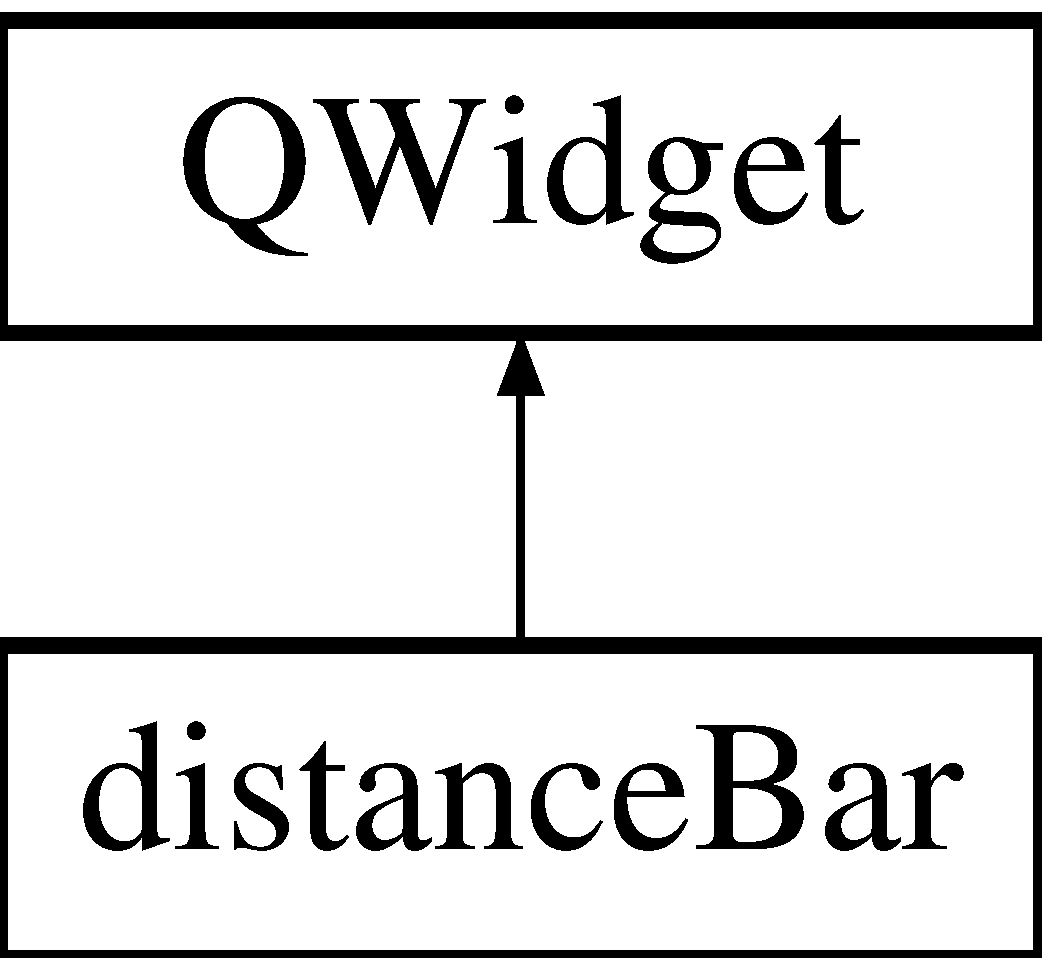
\includegraphics[height=2.000000cm]{classdistance_bar}
\end{center}
\end{figure}
\subsection*{Public Types}
\begin{DoxyCompactItemize}
\item 
\hypertarget{classdistance_bar_affb5e4f75675ad8818e25e20ad49a7bf}{enum {\bfseries bins} \{ {\bfseries S\+I\+G\+\_\+\+O\+O\+R} = 0, 
{\bfseries S\+I\+G\+\_\+\+F\+A\+R} = 1, 
{\bfseries S\+I\+G\+\_\+\+N\+E\+A\+R} = 2, 
{\bfseries S\+I\+G\+\_\+\+I\+M\+M\+E\+D\+I\+A\+T\+E} = 3
 \}}\label{classdistance_bar_affb5e4f75675ad8818e25e20ad49a7bf}

\end{DoxyCompactItemize}
\subsection*{Public Slots}
\begin{DoxyCompactItemize}
\item 
\hypertarget{classdistance_bar_a232f5295b631a95159790f6ba3fac61c}{void {\bfseries set\+Value} (int bin)}\label{classdistance_bar_a232f5295b631a95159790f6ba3fac61c}

\end{DoxyCompactItemize}
\subsection*{Public Member Functions}
\begin{DoxyCompactItemize}
\item 
\hypertarget{classdistance_bar_ab3c26ace6b9312e0ac8852eae724a852}{{\bfseries distance\+Bar} (qreal x, qreal y, Q\+Widget $\ast$parent=0, qreal width=D\+I\+S\+T\+A\+N\+C\+E\+\_\+\+D\+I\+S\+P\+L\+A\+Y\+\_\+\+W\+I\+D\+T\+H, qreal height=D\+I\+S\+T\+A\+N\+C\+E\+\_\+\+D\+I\+S\+P\+L\+A\+Y\+\_\+\+H\+E\+I\+G\+H\+T)}\label{classdistance_bar_ab3c26ace6b9312e0ac8852eae724a852}

\end{DoxyCompactItemize}
\subsection*{Protected Member Functions}
\begin{DoxyCompactItemize}
\item 
\hypertarget{classdistance_bar_ad193eaeef68b191b1eab951584efe9af}{void {\bfseries paint\+Event} (Q\+Paint\+Event $\ast$e)}\label{classdistance_bar_ad193eaeef68b191b1eab951584efe9af}

\end{DoxyCompactItemize}


The documentation for this class was generated from the following files\+:\begin{DoxyCompactItemize}
\item 
Distance\+Bar.\+h\item 
Distance\+Bar.\+cpp\end{DoxyCompactItemize}

\hypertarget{class_distance_widget}{\section{Distance\+Widget Class Reference}
\label{class_distance_widget}\index{Distance\+Widget@{Distance\+Widget}}
}
Inheritance diagram for Distance\+Widget\+:\begin{figure}[H]
\begin{center}
\leavevmode
\includegraphics[height=2.000000cm]{class_distance_widget}
\end{center}
\end{figure}
\subsection*{Public Slots}
\begin{DoxyCompactItemize}
\item 
\hypertarget{class_distance_widget_a43a6338696f4638ef9f57a16cc19a7c9}{void {\bfseries update\+Distance\+Label} (float db)}\label{class_distance_widget_a43a6338696f4638ef9f57a16cc19a7c9}

\item 
\hypertarget{class_distance_widget_af6d4db1f095c7f7356cc8776f1cd4da5}{void {\bfseries signal\+Loss} (bool is\+Connected)}\label{class_distance_widget_af6d4db1f095c7f7356cc8776f1cd4da5}

\end{DoxyCompactItemize}
\subsection*{Public Member Functions}
\begin{DoxyCompactItemize}
\item 
\hypertarget{class_distance_widget_a71ef67c16ce47d82a680c8c93961baaa}{{\bfseries Distance\+Widget} (\hyperlink{class_midas_thread}{Midas\+Thread} $\ast$main\+Thread, int width, int height, Q\+Widget $\ast$parent=0)}\label{class_distance_widget_a71ef67c16ce47d82a680c8c93961baaa}

\end{DoxyCompactItemize}


The documentation for this class was generated from the following files\+:\begin{DoxyCompactItemize}
\item 
Distance\+Widget.\+h\item 
Distance\+Widget.\+cpp\end{DoxyCompactItemize}

\hypertarget{class_draggable_widget}{\section{Draggable\+Widget Class Reference}
\label{class_draggable_widget}\index{Draggable\+Widget@{Draggable\+Widget}}
}


{\ttfamily \#include $<$Draggable\+Widget.\+h$>$}

Inheritance diagram for Draggable\+Widget\+:\begin{figure}[H]
\begin{center}
\leavevmode
\includegraphics[height=3.000000cm]{class_draggable_widget}
\end{center}
\end{figure}
\subsection*{Public Member Functions}
\begin{DoxyCompactItemize}
\item 
\hyperlink{class_draggable_widget_a2980778469300372e5ae6f275661e1ae}{Draggable\+Widget} (Q\+Widget $\ast$parent=0, Qt\+::\+Window\+Flags f=0)
\end{DoxyCompactItemize}
\subsection*{Protected Member Functions}
\begin{DoxyCompactItemize}
\item 
virtual void \hyperlink{class_draggable_widget_aff257b0727921eef2b9c306a524f3f07}{mouse\+Press\+Event} (Q\+Mouse\+Event $\ast$event)
\item 
virtual void \hyperlink{class_draggable_widget_a5fbd068a79a27a18eb8f7b3b8c58b9a1}{mouse\+Move\+Event} (Q\+Mouse\+Event $\ast$event)
\end{DoxyCompactItemize}


\subsection{Detailed Description}
This class represents a Widget that can be dragged using the mouse, by left-\/clicking the widget and dragging. 

\subsection{Constructor \& Destructor Documentation}
\hypertarget{class_draggable_widget_a2980778469300372e5ae6f275661e1ae}{\index{Draggable\+Widget@{Draggable\+Widget}!Draggable\+Widget@{Draggable\+Widget}}
\index{Draggable\+Widget@{Draggable\+Widget}!Draggable\+Widget@{Draggable\+Widget}}
\subsubsection[{Draggable\+Widget}]{\setlength{\rightskip}{0pt plus 5cm}Draggable\+Widget\+::\+Draggable\+Widget (
\begin{DoxyParamCaption}
\item[{Q\+Widget $\ast$}]{parent = {\ttfamily 0}, }
\item[{Qt\+::\+Window\+Flags}]{f = {\ttfamily 0}}
\end{DoxyParamCaption}
)}}\label{class_draggable_widget_a2980778469300372e5ae6f275661e1ae}
Constructs a \hyperlink{class_draggable_widget}{Draggable\+Widget} with a given parent (or no parent, if N\+U\+L\+L), and the specified flags f.


\begin{DoxyParams}{Parameters}
{\em parent} & The parent widget. \\
\hline
{\em f} & The window flags. \\
\hline
\end{DoxyParams}


\subsection{Member Function Documentation}
\hypertarget{class_draggable_widget_a5fbd068a79a27a18eb8f7b3b8c58b9a1}{\index{Draggable\+Widget@{Draggable\+Widget}!mouse\+Move\+Event@{mouse\+Move\+Event}}
\index{mouse\+Move\+Event@{mouse\+Move\+Event}!Draggable\+Widget@{Draggable\+Widget}}
\subsubsection[{mouse\+Move\+Event}]{\setlength{\rightskip}{0pt plus 5cm}void Draggable\+Widget\+::mouse\+Move\+Event (
\begin{DoxyParamCaption}
\item[{Q\+Mouse\+Event $\ast$}]{event}
\end{DoxyParamCaption}
)\hspace{0.3cm}{\ttfamily [protected]}, {\ttfamily [virtual]}}}\label{class_draggable_widget_a5fbd068a79a27a18eb8f7b3b8c58b9a1}
The event handler function that is called when the mouse moves over the widget. \hypertarget{class_draggable_widget_aff257b0727921eef2b9c306a524f3f07}{\index{Draggable\+Widget@{Draggable\+Widget}!mouse\+Press\+Event@{mouse\+Press\+Event}}
\index{mouse\+Press\+Event@{mouse\+Press\+Event}!Draggable\+Widget@{Draggable\+Widget}}
\subsubsection[{mouse\+Press\+Event}]{\setlength{\rightskip}{0pt plus 5cm}void Draggable\+Widget\+::mouse\+Press\+Event (
\begin{DoxyParamCaption}
\item[{Q\+Mouse\+Event $\ast$}]{event}
\end{DoxyParamCaption}
)\hspace{0.3cm}{\ttfamily [protected]}, {\ttfamily [virtual]}}}\label{class_draggable_widget_aff257b0727921eef2b9c306a524f3f07}
The event handler function that is called when the widget is clicked on by the mouse.


\begin{DoxyParams}{Parameters}
{\em event} & The mouse event structure, with information about the mouse press. \\
\hline
\end{DoxyParams}


The documentation for this class was generated from the following files\+:\begin{DoxyCompactItemize}
\item 
Draggable\+Widget.\+h\item 
Draggable\+Widget.\+cpp\end{DoxyCompactItemize}

\hypertarget{class_filter}{\section{Filter Class Reference}
\label{class_filter}\index{Filter@{Filter}}
}


{\ttfamily \#include $<$Filter.\+h$>$}

Inheritance diagram for Filter\+:\begin{figure}[H]
\begin{center}
\leavevmode
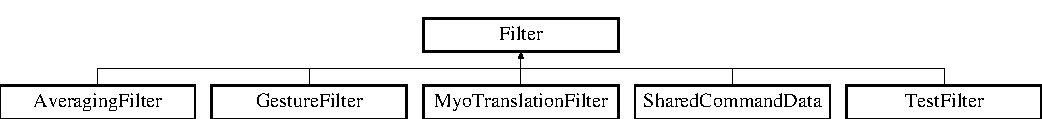
\includegraphics[height=1.577465cm]{class_filter}
\end{center}
\end{figure}
\subsection*{Public Member Functions}
\begin{DoxyCompactItemize}
\item 
virtual void \hyperlink{class_filter_a2f7afde0413c71a3e4947a0537ca8996}{process} ()=0
\item 
void \hyperlink{class_filter_a0d0f589585c96b4f0fcb1edb0454b958}{add\+Data\+As\+Input} (std\+::string name, boost\+::any value)
\item 
void \hyperlink{class_filter_a0b37fbd71bd25629f9476d61912ad038}{set\+Input} (filter\+Data\+Map input)
\item 
filter\+Data\+Map \hyperlink{class_filter_a3da920ba56f06a1ff15f6da0f298f8db}{get\+Output} ()
\item 
filter\+Status \hyperlink{class_filter_a547427e3f17dbb64a401881bed56088c}{get\+Filter\+Status} ()
\item 
filter\+Error \hyperlink{class_filter_a833dd72086569814cab3316c9354063a}{get\+Filter\+Error} ()
\item 
virtual filter\+Error \hyperlink{class_filter_a9ec2fbdbabb60c91e32048ebe386e372}{update\+Based\+On\+Profile} (\hyperlink{class_profile_manager}{Profile\+Manager} \&pm, std\+::string name)
\end{DoxyCompactItemize}
\subsection*{Protected Member Functions}
\begin{DoxyCompactItemize}
\item 
filter\+Data\+Map \hyperlink{class_filter_a8890993e559dc8b54c058b2666264ae8}{get\+Input} ()
\item 
void \hyperlink{class_filter_aedef5ef76a93b8263bcb62339b7b9fa9}{set\+Output} (filter\+Data\+Map output)
\item 
void \hyperlink{class_filter_ac38c830a3f01c16e86b4898153df5784}{clear\+Output} (void)
\item 
void \hyperlink{class_filter_a7e551c2ce698025792a385ced72525db}{set\+Filter\+Status} (filter\+Status status)
\item 
void \hyperlink{class_filter_ab8dc20b9548391941c4ea5effce254a9}{set\+Filter\+Error} (filter\+Error error)
\end{DoxyCompactItemize}


\subsection{Detailed Description}
\hyperlink{class_filter}{Filter} is an abstract class that is a component in a data flow pipeline. It takes in named data, processes the data, and then outputs the data. Filters can act as simple functions or they can be more complex, involving state or accumulated data. 

\subsection{Member Function Documentation}
\hypertarget{class_filter_a0d0f589585c96b4f0fcb1edb0454b958}{\index{Filter@{Filter}!add\+Data\+As\+Input@{add\+Data\+As\+Input}}
\index{add\+Data\+As\+Input@{add\+Data\+As\+Input}!Filter@{Filter}}
\subsubsection[{add\+Data\+As\+Input}]{\setlength{\rightskip}{0pt plus 5cm}void Filter\+::add\+Data\+As\+Input (
\begin{DoxyParamCaption}
\item[{std\+::string}]{name, }
\item[{boost\+::any}]{value}
\end{DoxyParamCaption}
)}}\label{class_filter_a0d0f589585c96b4f0fcb1edb0454b958}
Adds a new name-\/value pair to the input map of this filter. This value can be retrieved by name in the \hyperlink{class_filter_a2f7afde0413c71a3e4947a0537ca8996}{process()} function.


\begin{DoxyParams}{Parameters}
{\em name} & The name of the parameter. \\
\hline
{\em value} & The value corresponding with the name. \\
\hline
\end{DoxyParams}
\hypertarget{class_filter_ac38c830a3f01c16e86b4898153df5784}{\index{Filter@{Filter}!clear\+Output@{clear\+Output}}
\index{clear\+Output@{clear\+Output}!Filter@{Filter}}
\subsubsection[{clear\+Output}]{\setlength{\rightskip}{0pt plus 5cm}void Filter\+::clear\+Output (
\begin{DoxyParamCaption}
\item[{void}]{}
\end{DoxyParamCaption}
)\hspace{0.3cm}{\ttfamily [protected]}}}\label{class_filter_ac38c830a3f01c16e86b4898153df5784}
Clear the output of the filter. \hypertarget{class_filter_a833dd72086569814cab3316c9354063a}{\index{Filter@{Filter}!get\+Filter\+Error@{get\+Filter\+Error}}
\index{get\+Filter\+Error@{get\+Filter\+Error}!Filter@{Filter}}
\subsubsection[{get\+Filter\+Error}]{\setlength{\rightskip}{0pt plus 5cm}filter\+Error Filter\+::get\+Filter\+Error (
\begin{DoxyParamCaption}
{}
\end{DoxyParamCaption}
)}}\label{class_filter_a833dd72086569814cab3316c9354063a}
Retrieve an error code from the filter.

\begin{DoxyReturn}{Returns}
The error code of the filter after completion. 
\end{DoxyReturn}
\hypertarget{class_filter_a547427e3f17dbb64a401881bed56088c}{\index{Filter@{Filter}!get\+Filter\+Status@{get\+Filter\+Status}}
\index{get\+Filter\+Status@{get\+Filter\+Status}!Filter@{Filter}}
\subsubsection[{get\+Filter\+Status}]{\setlength{\rightskip}{0pt plus 5cm}filter\+Status Filter\+::get\+Filter\+Status (
\begin{DoxyParamCaption}
{}
\end{DoxyParamCaption}
)}}\label{class_filter_a547427e3f17dbb64a401881bed56088c}
Retrieve the status from the filter.

\begin{DoxyReturn}{Returns}
The status of the filter after completion. 
\end{DoxyReturn}
\hypertarget{class_filter_a8890993e559dc8b54c058b2666264ae8}{\index{Filter@{Filter}!get\+Input@{get\+Input}}
\index{get\+Input@{get\+Input}!Filter@{Filter}}
\subsubsection[{get\+Input}]{\setlength{\rightskip}{0pt plus 5cm}filter\+Data\+Map Filter\+::get\+Input (
\begin{DoxyParamCaption}
{}
\end{DoxyParamCaption}
)\hspace{0.3cm}{\ttfamily [protected]}}}\label{class_filter_a8890993e559dc8b54c058b2666264ae8}
Retrieve the input to the filter. Only a subclass of \hyperlink{class_filter}{Filter} can access the provided input.

\begin{DoxyReturn}{Returns}
The input to the filter. 
\end{DoxyReturn}
\hypertarget{class_filter_a3da920ba56f06a1ff15f6da0f298f8db}{\index{Filter@{Filter}!get\+Output@{get\+Output}}
\index{get\+Output@{get\+Output}!Filter@{Filter}}
\subsubsection[{get\+Output}]{\setlength{\rightskip}{0pt plus 5cm}filter\+Data\+Map Filter\+::get\+Output (
\begin{DoxyParamCaption}
{}
\end{DoxyParamCaption}
)}}\label{class_filter_a3da920ba56f06a1ff15f6da0f298f8db}
Retrieve the output from the filter.

\begin{DoxyReturn}{Returns}
A map of name-\/value pairs. 
\end{DoxyReturn}
\hypertarget{class_filter_a2f7afde0413c71a3e4947a0537ca8996}{\index{Filter@{Filter}!process@{process}}
\index{process@{process}!Filter@{Filter}}
\subsubsection[{process}]{\setlength{\rightskip}{0pt plus 5cm}virtual void Filter\+::process (
\begin{DoxyParamCaption}
{}
\end{DoxyParamCaption}
)\hspace{0.3cm}{\ttfamily [pure virtual]}}}\label{class_filter_a2f7afde0413c71a3e4947a0537ca8996}
This handles the processing of the data. It must get the named input, do something with the data, and then set the output. It is the responsibility of the implementing filter to properly set the output, status and error code before exiting this method. 

Implemented in \hyperlink{class_shared_command_data_a3085d27336d75f8e1974206585f831dd}{Shared\+Command\+Data}, \hyperlink{class_gesture_filter_a73231d8753e5d4cf04a208131819ad2c}{Gesture\+Filter}, \hyperlink{class_myo_translation_filter_a9f72c6ac36ed5ea26574db4b207a0597}{Myo\+Translation\+Filter}, \hyperlink{class_averaging_filter_accbc49506bc0c215ee8cb89b2a8b05f7}{Averaging\+Filter}, and \hyperlink{class_test_filter_acde9251dbdba4cd7913d3c641910a049}{Test\+Filter}.

\hypertarget{class_filter_ab8dc20b9548391941c4ea5effce254a9}{\index{Filter@{Filter}!set\+Filter\+Error@{set\+Filter\+Error}}
\index{set\+Filter\+Error@{set\+Filter\+Error}!Filter@{Filter}}
\subsubsection[{set\+Filter\+Error}]{\setlength{\rightskip}{0pt plus 5cm}void Filter\+::set\+Filter\+Error (
\begin{DoxyParamCaption}
\item[{filter\+Error}]{error}
\end{DoxyParamCaption}
)\hspace{0.3cm}{\ttfamily [protected]}}}\label{class_filter_ab8dc20b9548391941c4ea5effce254a9}
Set the error code of the filter.


\begin{DoxyParams}{Parameters}
{\em error} & The error code of the filter. \\
\hline
\end{DoxyParams}
\hypertarget{class_filter_a7e551c2ce698025792a385ced72525db}{\index{Filter@{Filter}!set\+Filter\+Status@{set\+Filter\+Status}}
\index{set\+Filter\+Status@{set\+Filter\+Status}!Filter@{Filter}}
\subsubsection[{set\+Filter\+Status}]{\setlength{\rightskip}{0pt plus 5cm}void Filter\+::set\+Filter\+Status (
\begin{DoxyParamCaption}
\item[{filter\+Status}]{status}
\end{DoxyParamCaption}
)\hspace{0.3cm}{\ttfamily [protected]}}}\label{class_filter_a7e551c2ce698025792a385ced72525db}
Set the status of the filter.


\begin{DoxyParams}{Parameters}
{\em status} & The status of the filter. \\
\hline
\end{DoxyParams}
\hypertarget{class_filter_a0b37fbd71bd25629f9476d61912ad038}{\index{Filter@{Filter}!set\+Input@{set\+Input}}
\index{set\+Input@{set\+Input}!Filter@{Filter}}
\subsubsection[{set\+Input}]{\setlength{\rightskip}{0pt plus 5cm}void Filter\+::set\+Input (
\begin{DoxyParamCaption}
\item[{filter\+Data\+Map}]{input}
\end{DoxyParamCaption}
)}}\label{class_filter_a0b37fbd71bd25629f9476d61912ad038}
Sets the input map for this filter. This can then be retrieved by the \hyperlink{class_filter_a2f7afde0413c71a3e4947a0537ca8996}{process()} function.


\begin{DoxyParams}{Parameters}
{\em input} & A map from string to boost\+::any of name-\/value pairs. \\
\hline
\end{DoxyParams}
\hypertarget{class_filter_aedef5ef76a93b8263bcb62339b7b9fa9}{\index{Filter@{Filter}!set\+Output@{set\+Output}}
\index{set\+Output@{set\+Output}!Filter@{Filter}}
\subsubsection[{set\+Output}]{\setlength{\rightskip}{0pt plus 5cm}void Filter\+::set\+Output (
\begin{DoxyParamCaption}
\item[{filter\+Data\+Map}]{output}
\end{DoxyParamCaption}
)\hspace{0.3cm}{\ttfamily [protected]}}}\label{class_filter_aedef5ef76a93b8263bcb62339b7b9fa9}
Set the output of the filter.


\begin{DoxyParams}{Parameters}
{\em output} & The map of name-\/value pairs. \\
\hline
\end{DoxyParams}
\hypertarget{class_filter_a9ec2fbdbabb60c91e32048ebe386e372}{\index{Filter@{Filter}!update\+Based\+On\+Profile@{update\+Based\+On\+Profile}}
\index{update\+Based\+On\+Profile@{update\+Based\+On\+Profile}!Filter@{Filter}}
\subsubsection[{update\+Based\+On\+Profile}]{\setlength{\rightskip}{0pt plus 5cm}filter\+Error Filter\+::update\+Based\+On\+Profile (
\begin{DoxyParamCaption}
\item[{{\bf Profile\+Manager} \&}]{pm, }
\item[{std\+::string}]{name}
\end{DoxyParamCaption}
)\hspace{0.3cm}{\ttfamily [virtual]}}}\label{class_filter_a9ec2fbdbabb60c91e32048ebe386e372}
Update filters internal mechanisms if the profile changes.

\begin{DoxyReturn}{Returns}
The error code of the filter after completion. 
\end{DoxyReturn}


Reimplemented in \hyperlink{class_myo_translation_filter_a1e1d3d6a3f1bf0d82d17367fc20d704d}{Myo\+Translation\+Filter}, and \hyperlink{class_gesture_filter_a65031496d7c7da33003499c75a63119c}{Gesture\+Filter}.



The documentation for this class was generated from the following files\+:\begin{DoxyCompactItemize}
\item 
Filter.\+h\item 
Filter.\+cpp\end{DoxyCompactItemize}

\hypertarget{class_filter_pipeline}{\section{Filter\+Pipeline Class Reference}
\label{class_filter_pipeline}\index{Filter\+Pipeline@{Filter\+Pipeline}}
}


{\ttfamily \#include $<$Filter\+Pipeline.\+h$>$}

\subsection*{Public Member Functions}
\begin{DoxyCompactItemize}
\item 
void \hyperlink{class_filter_pipeline_aa82ad15039984a23c7eda82d6627dab0}{register\+Filter} (\hyperlink{class_filter}{Filter} $\ast$filter)
\item 
void \hyperlink{class_filter_pipeline_aaf057248479d00b97538cd09f584452d}{start\+Pipeline} (filter\+Data\+Map input)
\item 
std\+::list$<$ \hyperlink{class_filter}{Filter} $\ast$ $>$ $\ast$ \hyperlink{class_filter_pipeline_aca193c07f273ee7ceb2c4f296b3e6b2f}{get\+Filters} (void)
\end{DoxyCompactItemize}


\subsection{Detailed Description}
The \hyperlink{class_filter_pipeline}{Filter\+Pipeline} class represents a linear sequence of filters through which data can flow. The data enters the pipeline and is passed into the first filter. The output of the first filter is piped into the second, and so on. 

\subsection{Member Function Documentation}
\hypertarget{class_filter_pipeline_aca193c07f273ee7ceb2c4f296b3e6b2f}{\index{Filter\+Pipeline@{Filter\+Pipeline}!get\+Filters@{get\+Filters}}
\index{get\+Filters@{get\+Filters}!Filter\+Pipeline@{Filter\+Pipeline}}
\subsubsection[{get\+Filters}]{\setlength{\rightskip}{0pt plus 5cm}std\+::list$<$ {\bf Filter} $\ast$ $>$ $\ast$ Filter\+Pipeline\+::get\+Filters (
\begin{DoxyParamCaption}
\item[{void}]{}
\end{DoxyParamCaption}
)}}\label{class_filter_pipeline_aca193c07f273ee7ceb2c4f296b3e6b2f}
Returns the list of registered filters.

\begin{DoxyReturn}{Returns}
The list of registered filters. 
\end{DoxyReturn}
\hypertarget{class_filter_pipeline_aa82ad15039984a23c7eda82d6627dab0}{\index{Filter\+Pipeline@{Filter\+Pipeline}!register\+Filter@{register\+Filter}}
\index{register\+Filter@{register\+Filter}!Filter\+Pipeline@{Filter\+Pipeline}}
\subsubsection[{register\+Filter}]{\setlength{\rightskip}{0pt plus 5cm}void Filter\+Pipeline\+::register\+Filter (
\begin{DoxyParamCaption}
\item[{{\bf Filter} $\ast$}]{filter}
\end{DoxyParamCaption}
)}}\label{class_filter_pipeline_aa82ad15039984a23c7eda82d6627dab0}
Registers a new filter with the pipeline. Adds it to the end of the pipeline.


\begin{DoxyParams}{Parameters}
{\em filter} & The filter to add to the pipeline. The input of the filter must match the output of the previous filter in the pipeline. \\
\hline
\end{DoxyParams}
\hypertarget{class_filter_pipeline_aaf057248479d00b97538cd09f584452d}{\index{Filter\+Pipeline@{Filter\+Pipeline}!start\+Pipeline@{start\+Pipeline}}
\index{start\+Pipeline@{start\+Pipeline}!Filter\+Pipeline@{Filter\+Pipeline}}
\subsubsection[{start\+Pipeline}]{\setlength{\rightskip}{0pt plus 5cm}void Filter\+Pipeline\+::start\+Pipeline (
\begin{DoxyParamCaption}
\item[{filter\+Data\+Map}]{input}
\end{DoxyParamCaption}
)}}\label{class_filter_pipeline_aaf057248479d00b97538cd09f584452d}
Starts the pipeline with the given input.


\begin{DoxyParams}{Parameters}
{\em input} & A map of name-\/value pairs that will be passed as the input to the first filter in the pipeline. \\
\hline
\end{DoxyParams}


The documentation for this class was generated from the following files\+:\begin{DoxyCompactItemize}
\item 
Filter\+Pipeline.\+h\item 
Filter\+Pipeline.\+cpp\end{DoxyCompactItemize}

\hypertarget{structgesture}{\section{gesture Struct Reference}
\label{structgesture}\index{gesture@{gesture}}
}
\subsection*{Public Attributes}
\begin{DoxyCompactItemize}
\item 
\hypertarget{structgesture_a604f792a5de91022f8343cff070192e5}{std\+::string {\bfseries type}}\label{structgesture_a604f792a5de91022f8343cff070192e5}

\item 
\hypertarget{structgesture_ac480b72b8e4be618a15caade626c130d}{std\+::string {\bfseries name}}\label{structgesture_ac480b72b8e4be618a15caade626c130d}

\end{DoxyCompactItemize}


The documentation for this struct was generated from the following file\+:\begin{DoxyCompactItemize}
\item 
Profile\+Manager.\+h\end{DoxyCompactItemize}

\hypertarget{class_gesture_filter}{\section{Gesture\+Filter Class Reference}
\label{class_gesture_filter}\index{Gesture\+Filter@{Gesture\+Filter}}
}


{\ttfamily \#include $<$Gesture\+Filter.\+h$>$}

Inheritance diagram for Gesture\+Filter\+:\begin{figure}[H]
\begin{center}
\leavevmode
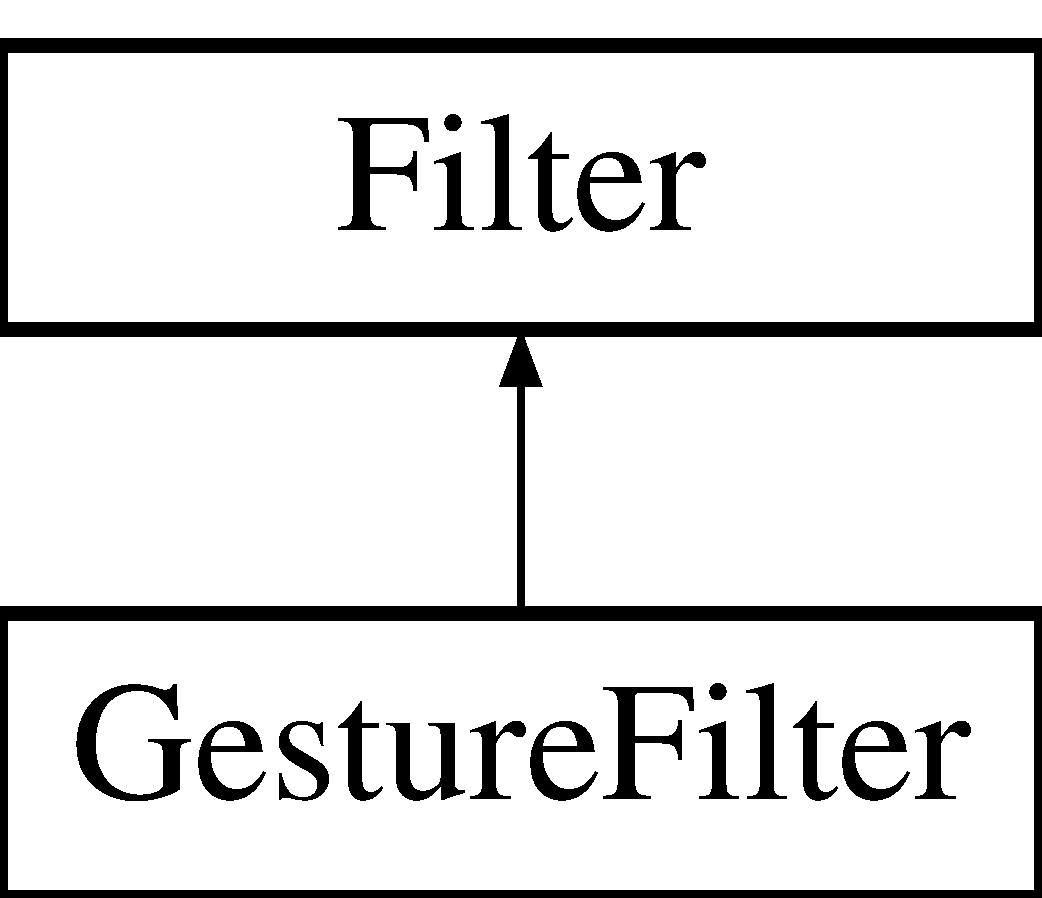
\includegraphics[height=2.000000cm]{class_gesture_filter}
\end{center}
\end{figure}
\subsection*{Public Member Functions}
\begin{DoxyCompactItemize}
\item 
\hyperlink{class_gesture_filter_a7ec8f885370e67e108bd1f767e9f2769}{Gesture\+Filter} (\hyperlink{class_control_state}{Control\+State} $\ast$control\+State, clock\+\_\+t time\+Del, \hyperlink{class_main_g_u_i}{Main\+G\+U\+I} $\ast$main\+Gui\+Handle)
\item 
void \hyperlink{class_gesture_filter_a73231d8753e5d4cf04a208131819ad2c}{process} ()
\item 
\hypertarget{class_gesture_filter_a836ba016c9b8edf33c4511881218f7cf}{filter\+Data\+Map {\bfseries get\+Extra\+Data\+For\+S\+C\+D} ()}\label{class_gesture_filter_a836ba016c9b8edf33c4511881218f7cf}

\item 
filter\+Error \hyperlink{class_gesture_filter_a65031496d7c7da33003499c75a63119c}{update\+Based\+On\+Profile} (\hyperlink{class_profile_manager}{Profile\+Manager} \&pm, std\+::string name)
\item 
\hyperlink{class_gesture_seq_recorder}{Gesture\+Seq\+Recorder} $\ast$ \hyperlink{class_gesture_filter_af77130b2c3dbaa45a78ea6aaa39152dd}{get\+Gesture\+Seq\+Recorder} ()
\end{DoxyCompactItemize}
\subsection*{Static Public Member Functions}
\begin{DoxyCompactItemize}
\item 
\hypertarget{class_gesture_filter_ac778bc1d58a29b60b644252818a7d85f}{static void {\bfseries handle\+State\+Change} (\hyperlink{structcommand_data}{command\+Data} response)}\label{class_gesture_filter_ac778bc1d58a29b60b644252818a7d85f}

\end{DoxyCompactItemize}
\subsection*{Friends}
\begin{DoxyCompactItemize}
\item 
\hypertarget{class_gesture_filter_ad4a43c3f8911f427cf34b7d6d8c4e914}{void {\bfseries setup\+Callback\+Thread} (\hyperlink{class_gesture_filter}{Gesture\+Filter} $\ast$gf)}\label{class_gesture_filter_ad4a43c3f8911f427cf34b7d6d8c4e914}

\item 
\hypertarget{class_gesture_filter_adc082e2eed06986940cf0846b9f96968}{void {\bfseries callback\+Thread\+Wrapper} (\hyperlink{class_gesture_filter}{Gesture\+Filter} $\ast$gf)}\label{class_gesture_filter_adc082e2eed06986940cf0846b9f96968}

\end{DoxyCompactItemize}
\subsection*{Additional Inherited Members}


\subsection{Detailed Description}
Consult \hyperlink{_filter_8h_source}{Filter.\+h} for concepts regarding Filters.

A filter specific to the Myo armband that handles changing the application state when a certain gesture is performed, and translates from Myo gestures to mouse and keyboard commands. Furthermore, helps to prevent against false positive gesture recognition by forcing the user to hold a gesture for a certain amount of time before registering it. 

\subsection{Constructor \& Destructor Documentation}
\hypertarget{class_gesture_filter_a7ec8f885370e67e108bd1f767e9f2769}{\index{Gesture\+Filter@{Gesture\+Filter}!Gesture\+Filter@{Gesture\+Filter}}
\index{Gesture\+Filter@{Gesture\+Filter}!Gesture\+Filter@{Gesture\+Filter}}
\subsubsection[{Gesture\+Filter}]{\setlength{\rightskip}{0pt plus 5cm}Gesture\+Filter\+::\+Gesture\+Filter (
\begin{DoxyParamCaption}
\item[{{\bf Control\+State} $\ast$}]{control\+State, }
\item[{clock\+\_\+t}]{time\+Del, }
\item[{{\bf Main\+G\+U\+I} $\ast$}]{main\+Gui\+Handle}
\end{DoxyParamCaption}
)}}\label{class_gesture_filter_a7ec8f885370e67e108bd1f767e9f2769}
The constructor for the \hyperlink{class_gesture_filter}{Gesture\+Filter}. It takes a \hyperlink{class_control_state}{Control\+State} handle so that the state of the application can be changed by gesture control. It sets the time that must occur before a gesture is registered.


\begin{DoxyParams}{Parameters}
{\em control\+State} & A handle to the \hyperlink{class_control_state}{Control\+State} object that manages application state. \\
\hline
{\em time\+Del} & The time that a user must hold a gesture before it is registered. \\
\hline
\end{DoxyParams}


\subsection{Member Function Documentation}
\hypertarget{class_gesture_filter_af77130b2c3dbaa45a78ea6aaa39152dd}{\index{Gesture\+Filter@{Gesture\+Filter}!get\+Gesture\+Seq\+Recorder@{get\+Gesture\+Seq\+Recorder}}
\index{get\+Gesture\+Seq\+Recorder@{get\+Gesture\+Seq\+Recorder}!Gesture\+Filter@{Gesture\+Filter}}
\subsubsection[{get\+Gesture\+Seq\+Recorder}]{\setlength{\rightskip}{0pt plus 5cm}{\bf Gesture\+Seq\+Recorder}$\ast$ Gesture\+Filter\+::get\+Gesture\+Seq\+Recorder (
\begin{DoxyParamCaption}
{}
\end{DoxyParamCaption}
)\hspace{0.3cm}{\ttfamily [inline]}}}\label{class_gesture_filter_af77130b2c3dbaa45a78ea6aaa39152dd}
return actual handle to gest\+Seq\+Recorder \hypertarget{class_gesture_filter_a73231d8753e5d4cf04a208131819ad2c}{\index{Gesture\+Filter@{Gesture\+Filter}!process@{process}}
\index{process@{process}!Gesture\+Filter@{Gesture\+Filter}}
\subsubsection[{process}]{\setlength{\rightskip}{0pt plus 5cm}void Gesture\+Filter\+::process (
\begin{DoxyParamCaption}
{}
\end{DoxyParamCaption}
)\hspace{0.3cm}{\ttfamily [virtual]}}}\label{class_gesture_filter_a73231d8753e5d4cf04a208131819ad2c}
This is the \hyperlink{class_gesture_filter_a73231d8753e5d4cf04a208131819ad2c}{process()} function that overrides the base \hyperlink{class_filter}{Filter} class \hyperlink{class_gesture_filter_a73231d8753e5d4cf04a208131819ad2c}{process()}. It handles the logic of the filter. It translates gestures to the corresponding mouse and keyboard commands, handles changing the application state, and enforces the timing restriction that prevents, or rather reduces the chance of, false positive gestures from being recognized. 

Implements \hyperlink{class_filter_a2f7afde0413c71a3e4947a0537ca8996}{Filter}.

\hypertarget{class_gesture_filter_a65031496d7c7da33003499c75a63119c}{\index{Gesture\+Filter@{Gesture\+Filter}!update\+Based\+On\+Profile@{update\+Based\+On\+Profile}}
\index{update\+Based\+On\+Profile@{update\+Based\+On\+Profile}!Gesture\+Filter@{Gesture\+Filter}}
\subsubsection[{update\+Based\+On\+Profile}]{\setlength{\rightskip}{0pt plus 5cm}filter\+Error Gesture\+Filter\+::update\+Based\+On\+Profile (
\begin{DoxyParamCaption}
\item[{{\bf Profile\+Manager} \&}]{pm, }
\item[{std\+::string}]{name}
\end{DoxyParamCaption}
)\hspace{0.3cm}{\ttfamily [virtual]}}}\label{class_gesture_filter_a65031496d7c7da33003499c75a63119c}
Update filters internal mechanisms if the profile changes.

\begin{DoxyReturn}{Returns}
The error code of the filter after completion. 
\end{DoxyReturn}


Reimplemented from \hyperlink{class_filter_a9ec2fbdbabb60c91e32048ebe386e372}{Filter}.



The documentation for this class was generated from the following files\+:\begin{DoxyCompactItemize}
\item 
Gesture\+Filter.\+h\item 
Gesture\+Filter.\+cpp\end{DoxyCompactItemize}

\hypertarget{class_gesture_hold_mode_action}{\section{Gesture\+Hold\+Mode\+Action Class Reference}
\label{class_gesture_hold_mode_action}\index{Gesture\+Hold\+Mode\+Action@{Gesture\+Hold\+Mode\+Action}}
}
\subsection*{Public Member Functions}
\begin{DoxyCompactItemize}
\item 
\hypertarget{class_gesture_hold_mode_action_aaf5a4037ba4e75fcd62598444ba4fb5e}{{\bfseries Gesture\+Hold\+Mode\+Action} (unsigned int min\+Interval\+Len)}\label{class_gesture_hold_mode_action_aaf5a4037ba4e75fcd62598444ba4fb5e}

\item 
\hypertarget{class_gesture_hold_mode_action_ae69e9d3ea0730c541b55a35addb79aee}{void {\bfseries clear\+Map} ()}\label{class_gesture_hold_mode_action_ae69e9d3ea0730c541b55a35addb79aee}

\item 
\hypertarget{class_gesture_hold_mode_action_a65594540731af2676f2789bd90ffaa31}{bool {\bfseries add\+To\+Action\+Map} (\hyperlink{structangle_data}{angle\+Data} ad, kybd\+Cmds \hyperlink{structcommand}{command})}\label{class_gesture_hold_mode_action_a65594540731af2676f2789bd90ffaa31}

\item 
\hypertarget{class_gesture_hold_mode_action_aa4294b9e71260e93e8f1e37002254a24}{kybd\+Cmds {\bfseries get\+Action} (\hyperlink{structangle_data}{angle\+Data} ad)}\label{class_gesture_hold_mode_action_aa4294b9e71260e93e8f1e37002254a24}

\end{DoxyCompactItemize}


The documentation for this class was generated from the following files\+:\begin{DoxyCompactItemize}
\item 
Gesture\+Hold\+Mode\+Action.\+h\item 
Gesture\+Hold\+Mode\+Action.\+cpp\end{DoxyCompactItemize}

\hypertarget{class_gesture_seq_recorder}{\section{Gesture\+Seq\+Recorder Class Reference}
\label{class_gesture_seq_recorder}\index{Gesture\+Seq\+Recorder@{Gesture\+Seq\+Recorder}}
}
\subsection*{Public Member Functions}
\begin{DoxyCompactItemize}
\item 
\hyperlink{class_gesture_seq_recorder_a89617ae8b04c44b33006f14c388ed248}{Gesture\+Seq\+Recorder} (\hyperlink{class_control_state}{Control\+State} $\ast$control\+State\+Handle, \hyperlink{class_main_g_u_i}{Main\+G\+U\+I} $\ast$main\+Gui\+Handle, \hyperlink{class_sequence_image_manager}{Sequence\+Image\+Manager} image\+Manager)
\item 
\hypertarget{class_gesture_seq_recorder_a3aab363a46e6c19c494de8572c039577}{void {\bfseries unregister\+All} ()}\label{class_gesture_seq_recorder_a3aab363a46e6c19c494de8572c039577}

\item 
Sequence\+Status \hyperlink{class_gesture_seq_recorder_a5a2febae745433a770227ab6bdeb7630}{register\+Sequence} (midas\+Mode mode, sequence seq, \hyperlink{structcommand_data}{command\+Data} seq\+Response, std\+::string name)
\item 
Sequence\+Status \hyperlink{class_gesture_seq_recorder_aa64d6f130b1937fea36a8d6aa4362c6b}{progress\+Sequence} (Pose\+::\+Type \hyperlink{structgesture}{gesture}, \hyperlink{class_control_state}{Control\+State} state, \hyperlink{structcommand_data}{command\+Data} \&response)
\item 
void \hyperlink{class_gesture_seq_recorder_ad67f5a6b8d22d6895b42e4ec47be3562}{progress\+Sequence\+Time} (int delta, \hyperlink{structcommand_data}{command\+Data} \&response)
\item 
void \hyperlink{class_gesture_seq_recorder_a32b78602089532a166879ed9a27fac2e}{check\+Progress\+Base\+Time} ()
\item 
void \hyperlink{class_gesture_seq_recorder_a0692d367b4429900c3ab05dfa36990fa}{empty\+Active\+Sequences} ()
\item 
void \hyperlink{class_gesture_seq_recorder_a0a5fd083e4e0ed75d6f07415a6e5cea1}{set\+Progress\+Max\+Delta\+Time} (clock\+\_\+t new\+Time)
\item 
clock\+\_\+t \hyperlink{class_gesture_seq_recorder_aa5de7ea6101ab22ba2a14f0f718a6370}{get\+Progress\+Max\+Delta\+Time} (void)
\item 
void \hyperlink{class_gesture_seq_recorder_a65164a6763e30c37677cefe5aff5a36b}{print\+Status} (bool verbose=false)
\item 
void \hyperlink{class_gesture_seq_recorder_ad27d85ae4783eda851c692ffb542efdb}{update\+Gui\+Sequences} ()
\end{DoxyCompactItemize}


\subsection{Constructor \& Destructor Documentation}
\hypertarget{class_gesture_seq_recorder_a89617ae8b04c44b33006f14c388ed248}{\index{Gesture\+Seq\+Recorder@{Gesture\+Seq\+Recorder}!Gesture\+Seq\+Recorder@{Gesture\+Seq\+Recorder}}
\index{Gesture\+Seq\+Recorder@{Gesture\+Seq\+Recorder}!Gesture\+Seq\+Recorder@{Gesture\+Seq\+Recorder}}
\subsubsection[{Gesture\+Seq\+Recorder}]{\setlength{\rightskip}{0pt plus 5cm}Gesture\+Seq\+Recorder\+::\+Gesture\+Seq\+Recorder (
\begin{DoxyParamCaption}
\item[{{\bf Control\+State} $\ast$}]{control\+State\+Handle, }
\item[{{\bf Main\+G\+U\+I} $\ast$}]{main\+Gui\+Handle, }
\item[{{\bf Sequence\+Image\+Manager}}]{image\+Manager}
\end{DoxyParamCaption}
)}}\label{class_gesture_seq_recorder_a89617ae8b04c44b33006f14c388ed248}
Constructors/\+Destructor 

\subsection{Member Function Documentation}
\hypertarget{class_gesture_seq_recorder_a32b78602089532a166879ed9a27fac2e}{\index{Gesture\+Seq\+Recorder@{Gesture\+Seq\+Recorder}!check\+Progress\+Base\+Time@{check\+Progress\+Base\+Time}}
\index{check\+Progress\+Base\+Time@{check\+Progress\+Base\+Time}!Gesture\+Seq\+Recorder@{Gesture\+Seq\+Recorder}}
\subsubsection[{check\+Progress\+Base\+Time}]{\setlength{\rightskip}{0pt plus 5cm}void Gesture\+Seq\+Recorder\+::check\+Progress\+Base\+Time (
\begin{DoxyParamCaption}
{}
\end{DoxyParamCaption}
)}}\label{class_gesture_seq_recorder_a32b78602089532a166879ed9a27fac2e}
Called to check against progress\+Base\+Time if any sequences are active, so that a sequence can be cleared if timed out, without an asynchronous gesture update. \hypertarget{class_gesture_seq_recorder_a0692d367b4429900c3ab05dfa36990fa}{\index{Gesture\+Seq\+Recorder@{Gesture\+Seq\+Recorder}!empty\+Active\+Sequences@{empty\+Active\+Sequences}}
\index{empty\+Active\+Sequences@{empty\+Active\+Sequences}!Gesture\+Seq\+Recorder@{Gesture\+Seq\+Recorder}}
\subsubsection[{empty\+Active\+Sequences}]{\setlength{\rightskip}{0pt plus 5cm}void Gesture\+Seq\+Recorder\+::empty\+Active\+Sequences (
\begin{DoxyParamCaption}
{}
\end{DoxyParamCaption}
)}}\label{class_gesture_seq_recorder_a0692d367b4429900c3ab05dfa36990fa}
Empty the references to sequences that were active, and set progress of each to 0. \hypertarget{class_gesture_seq_recorder_aa5de7ea6101ab22ba2a14f0f718a6370}{\index{Gesture\+Seq\+Recorder@{Gesture\+Seq\+Recorder}!get\+Progress\+Max\+Delta\+Time@{get\+Progress\+Max\+Delta\+Time}}
\index{get\+Progress\+Max\+Delta\+Time@{get\+Progress\+Max\+Delta\+Time}!Gesture\+Seq\+Recorder@{Gesture\+Seq\+Recorder}}
\subsubsection[{get\+Progress\+Max\+Delta\+Time}]{\setlength{\rightskip}{0pt plus 5cm}clock\+\_\+t Gesture\+Seq\+Recorder\+::get\+Progress\+Max\+Delta\+Time (
\begin{DoxyParamCaption}
\item[{void}]{}
\end{DoxyParamCaption}
)}}\label{class_gesture_seq_recorder_aa5de7ea6101ab22ba2a14f0f718a6370}
Accessor.

\begin{DoxyReturn}{Returns}
Value of progress\+Max\+Delta\+Time. 
\end{DoxyReturn}
\hypertarget{class_gesture_seq_recorder_a65164a6763e30c37677cefe5aff5a36b}{\index{Gesture\+Seq\+Recorder@{Gesture\+Seq\+Recorder}!print\+Status@{print\+Status}}
\index{print\+Status@{print\+Status}!Gesture\+Seq\+Recorder@{Gesture\+Seq\+Recorder}}
\subsubsection[{print\+Status}]{\setlength{\rightskip}{0pt plus 5cm}void Gesture\+Seq\+Recorder\+::print\+Status (
\begin{DoxyParamCaption}
\item[{bool}]{verbose = {\ttfamily false}}
\end{DoxyParamCaption}
)}}\label{class_gesture_seq_recorder_a65164a6763e30c37677cefe5aff5a36b}
Print out a list of all active sequences, and possibly their progress, and next gesture required to proceed!


\begin{DoxyParams}{Parameters}
{\em verbose} & If true, prints progress and next gesture in sequence on top of active status.\\
\hline
\end{DoxyParams}
T\+O\+D\+O\+: This is the beginning of the code which overlays graphically action data to the user. Just using printing temporarily. \hypertarget{class_gesture_seq_recorder_aa64d6f130b1937fea36a8d6aa4362c6b}{\index{Gesture\+Seq\+Recorder@{Gesture\+Seq\+Recorder}!progress\+Sequence@{progress\+Sequence}}
\index{progress\+Sequence@{progress\+Sequence}!Gesture\+Seq\+Recorder@{Gesture\+Seq\+Recorder}}
\subsubsection[{progress\+Sequence}]{\setlength{\rightskip}{0pt plus 5cm}Sequence\+Status Gesture\+Seq\+Recorder\+::progress\+Sequence (
\begin{DoxyParamCaption}
\item[{Pose\+::\+Type}]{gesture, }
\item[{{\bf Control\+State}}]{state, }
\item[{{\bf command\+Data} \&}]{response}
\end{DoxyParamCaption}
)}}\label{class_gesture_seq_recorder_aa64d6f130b1937fea36a8d6aa4362c6b}
Given a gesture, attempt to progress through any registered sequences, that match the mode of the control\+State.


\begin{DoxyParams}{Parameters}
{\em gesture} & The recorded gesture that is being used to compare with the registered sequences. \\
\hline
{\em state} & The \hyperlink{class_control_state}{Control\+State} handle to determine the current midas\+Mode of the system, thereby knowing which registered sequence list to search through. \\
\hline
{\em response} & The \hyperlink{structcommand_data}{command\+Data} that is populated by the function. Holding a type of N\+O\+N\+E means that no sequence was completed. However, if it's not N\+O\+N\+E, it holds the response that was registered against the completed sequence. \\
\hline
\end{DoxyParams}
\begin{DoxyReturn}{Returns}
Sequence\+Status associated status information to inform caller of success/lack there of 
\end{DoxyReturn}
\hypertarget{class_gesture_seq_recorder_ad67f5a6b8d22d6895b42e4ec47be3562}{\index{Gesture\+Seq\+Recorder@{Gesture\+Seq\+Recorder}!progress\+Sequence\+Time@{progress\+Sequence\+Time}}
\index{progress\+Sequence\+Time@{progress\+Sequence\+Time}!Gesture\+Seq\+Recorder@{Gesture\+Seq\+Recorder}}
\subsubsection[{progress\+Sequence\+Time}]{\setlength{\rightskip}{0pt plus 5cm}void Gesture\+Seq\+Recorder\+::progress\+Sequence\+Time (
\begin{DoxyParamCaption}
\item[{int}]{delta, }
\item[{{\bf command\+Data} \&}]{response}
\end{DoxyParamCaption}
)}}\label{class_gesture_seq_recorder_ad67f5a6b8d22d6895b42e4ec47be3562}
To handle tap/hold differentiation, this should be called to notify the Seq\+Recorder that a certain amount of time has passed. If a certain amount of time passes while a user is holding a specific pose, then they are deemed to be holding it, otherwise they have tapped it. This function will continually decrement the hold timer, and if it reaches 0, it will clear any active sequences that were supposed to have a 'tap' action, and will progress any sequences that have a 'hold' action.


\begin{DoxyParams}{Parameters}
{\em delta} & The amount of time in ms indicated to have passed. \\
\hline
{\em response} & The \hyperlink{structcommand_data}{command\+Data} that is populated by the function. Holding a type of N\+O\+N\+E means that no sequence was completed. However, if it's not N\+O\+N\+E, it holds the response that was registered against the completed sequence. \\
\hline
\end{DoxyParams}
\begin{DoxyReturn}{Returns}
Sequence\+Status The status of the progression. S\+U\+C\+C\+E\+S\+S is typical and wanted. 
\end{DoxyReturn}
\hypertarget{class_gesture_seq_recorder_a5a2febae745433a770227ab6bdeb7630}{\index{Gesture\+Seq\+Recorder@{Gesture\+Seq\+Recorder}!register\+Sequence@{register\+Sequence}}
\index{register\+Sequence@{register\+Sequence}!Gesture\+Seq\+Recorder@{Gesture\+Seq\+Recorder}}
\subsubsection[{register\+Sequence}]{\setlength{\rightskip}{0pt plus 5cm}Sequence\+Status Gesture\+Seq\+Recorder\+::register\+Sequence (
\begin{DoxyParamCaption}
\item[{midas\+Mode}]{mode, }
\item[{sequence}]{seq, }
\item[{{\bf command\+Data}}]{seq\+Response, }
\item[{std\+::string}]{name}
\end{DoxyParamCaption}
)}}\label{class_gesture_seq_recorder_a5a2febae745433a770227ab6bdeb7630}
Register a sequence of gestures with this call. A registered sequence is associated with a midas\+Mode. When in that mode, any progression of gestures from the Myo will be compared to all associated and registered sequences, and if any are succesfully completed, the registered \hyperlink{structcommand_data}{command\+Data} will be returned to the caller. N\+O\+T\+E\+: Can only register sequences with Seq\+Elements of Pose\+Length I\+M\+M\+E\+D\+I\+A\+T\+E if the sequence is of length one. This could be changed in the future if deemed necessary, but this allows progress\+Sequence to be unnafected by this special case.


\begin{DoxyParams}{Parameters}
{\em mode} & The midas\+Mode that the caller is registering the sequence against. \\
\hline
{\em seq} & The sequence (std\+::vector$<$\+Pose\+::\+Type$>$) of gestures to register \\
\hline
{\em seq\+Response} & The desired response to activate if the sequence is recognized while in the registered mode. \\
\hline
\end{DoxyParams}
\begin{DoxyReturn}{Returns}
Sequence\+Status associated status information to inform caller of success/lack there of 
\end{DoxyReturn}
\hypertarget{class_gesture_seq_recorder_a0a5fd083e4e0ed75d6f07415a6e5cea1}{\index{Gesture\+Seq\+Recorder@{Gesture\+Seq\+Recorder}!set\+Progress\+Max\+Delta\+Time@{set\+Progress\+Max\+Delta\+Time}}
\index{set\+Progress\+Max\+Delta\+Time@{set\+Progress\+Max\+Delta\+Time}!Gesture\+Seq\+Recorder@{Gesture\+Seq\+Recorder}}
\subsubsection[{set\+Progress\+Max\+Delta\+Time}]{\setlength{\rightskip}{0pt plus 5cm}void Gesture\+Seq\+Recorder\+::set\+Progress\+Max\+Delta\+Time (
\begin{DoxyParamCaption}
\item[{clock\+\_\+t}]{new\+Time}
\end{DoxyParamCaption}
)}}\label{class_gesture_seq_recorder_a0a5fd083e4e0ed75d6f07415a6e5cea1}
Modifier.


\begin{DoxyParams}{Parameters}
{\em new\+Time} & The new progress\+Max\+Delta\+Time. \\
\hline
\end{DoxyParams}
\hypertarget{class_gesture_seq_recorder_ad27d85ae4783eda851c692ffb542efdb}{\index{Gesture\+Seq\+Recorder@{Gesture\+Seq\+Recorder}!update\+Gui\+Sequences@{update\+Gui\+Sequences}}
\index{update\+Gui\+Sequences@{update\+Gui\+Sequences}!Gesture\+Seq\+Recorder@{Gesture\+Seq\+Recorder}}
\subsubsection[{update\+Gui\+Sequences}]{\setlength{\rightskip}{0pt plus 5cm}void Gesture\+Seq\+Recorder\+::update\+Gui\+Sequences (
\begin{DoxyParamCaption}
{}
\end{DoxyParamCaption}
)}}\label{class_gesture_seq_recorder_ad27d85ae4783eda851c692ffb542efdb}
Updates the sequence displayer G\+U\+I with the latest sequence information. This should be called upon any update to the sequences. 

The documentation for this class was generated from the following files\+:\begin{DoxyCompactItemize}
\item 
Gesture\+Seq\+Recorder.\+h\item 
Gesture\+Seq\+Recorder.\+cpp\end{DoxyCompactItemize}

\hypertarget{class_gesture_signaller}{\section{Gesture\+Signaller Class Reference}
\label{class_gesture_signaller}\index{Gesture\+Signaller@{Gesture\+Signaller}}
}


{\ttfamily \#include $<$Gesture\+Signaller.\+h$>$}

Inheritance diagram for Gesture\+Signaller\+:\begin{figure}[H]
\begin{center}
\leavevmode
\includegraphics[height=2.000000cm]{class_gesture_signaller}
\end{center}
\end{figure}
\subsection*{Public Slots}
\begin{DoxyCompactItemize}
\item 
\hypertarget{class_gesture_signaller_a274c5b162f1067b917c141976a178c00}{void {\bfseries handle\+Show\+All\+Toggle} (bool show\+All)}\label{class_gesture_signaller_a274c5b162f1067b917c141976a178c00}

\end{DoxyCompactItemize}
\subsection*{Signals}
\begin{DoxyCompactItemize}
\item 
\hypertarget{class_gesture_signaller_a88fca41be5e113483e4224495fcd73c7}{void {\bfseries emit\+Register\+Sequence} (int, Q\+String, std\+::vector$<$ \hyperlink{structsequence_image_set}{sequence\+Image\+Set} $>$)}\label{class_gesture_signaller_a88fca41be5e113483e4224495fcd73c7}

\item 
\hypertarget{class_gesture_signaller_abe4f99d4cf0f7e88fd6284312e9b2985}{void {\bfseries emit\+Show\+Sequences} (std\+::vector$<$ \hyperlink{structsequence_progress_data}{sequence\+Progress\+Data} $>$)}\label{class_gesture_signaller_abe4f99d4cf0f7e88fd6284312e9b2985}

\item 
\hypertarget{class_gesture_signaller_a908109e51f88924f810a8d66769b0abe}{void {\bfseries emit\+State\+String} (Q\+String)}\label{class_gesture_signaller_a908109e51f88924f810a8d66769b0abe}

\item 
\hypertarget{class_gesture_signaller_aa613d8732a6427f9ec8f759a34905b31}{void {\bfseries emit\+Pose\+Images} (std\+::vector$<$ \hyperlink{structsequence_image_set}{sequence\+Image\+Set} $>$)}\label{class_gesture_signaller_aa613d8732a6427f9ec8f759a34905b31}

\item 
\hypertarget{class_gesture_signaller_a719191283f7644548430b353f8b1a453}{void {\bfseries emit\+Toggle\+Keyboard} ()}\label{class_gesture_signaller_a719191283f7644548430b353f8b1a453}

\end{DoxyCompactItemize}
\subsection*{Public Member Functions}
\begin{DoxyCompactItemize}
\item 
\hypertarget{class_gesture_signaller_a8516517898a400a28f900eec60c8d3e8}{bool {\bfseries get\+Show\+All} ()}\label{class_gesture_signaller_a8516517898a400a28f900eec60c8d3e8}

\end{DoxyCompactItemize}


\subsection{Detailed Description}
The \hyperlink{class_gesture_signaller}{Gesture\+Signaller} class handles the communication between the Midas sequence logic and the \hyperlink{class_sequence_displayer}{Sequence\+Displayer} G\+U\+I. 

The documentation for this class was generated from the following files\+:\begin{DoxyCompactItemize}
\item 
Gesture\+Signaller.\+h\item 
Gesture\+Signaller.\+cpp\end{DoxyCompactItemize}

\hypertarget{structhold}{\section{hold Struct Reference}
\label{structhold}\index{hold@{hold}}
}
\subsection*{Public Attributes}
\begin{DoxyCompactItemize}
\item 
\hypertarget{structhold_a327925dd3da3b0efcf737fcd7fa43d4b}{std\+::string {\bfseries gesture}}\label{structhold_a327925dd3da3b0efcf737fcd7fa43d4b}

\item 
\hypertarget{structhold_a19b8b7d6dbc64ff80e75582738b70c83}{std\+::vector$<$ \hyperlink{structangle_action}{angle\+Action} $>$ {\bfseries angles}}\label{structhold_a19b8b7d6dbc64ff80e75582738b70c83}

\end{DoxyCompactItemize}


The documentation for this struct was generated from the following file\+:\begin{DoxyCompactItemize}
\item 
Profile\+Manager.\+h\end{DoxyCompactItemize}

\hypertarget{class_info_indicator}{\section{Info\+Indicator Class Reference}
\label{class_info_indicator}\index{Info\+Indicator@{Info\+Indicator}}
}
Inheritance diagram for Info\+Indicator\+:\begin{figure}[H]
\begin{center}
\leavevmode
\includegraphics[height=2.000000cm]{class_info_indicator}
\end{center}
\end{figure}
\subsection*{Public Slots}
\begin{DoxyCompactItemize}
\item 
\hypertarget{class_info_indicator_a838e6276592edd2a99f1d0eaf18fa644}{void {\bfseries handle\+Update\+State} (Q\+String state\+Label)}\label{class_info_indicator_a838e6276592edd2a99f1d0eaf18fa644}

\end{DoxyCompactItemize}
\subsection*{Signals}
\begin{DoxyCompactItemize}
\item 
\hypertarget{class_info_indicator_ab30bb585ee9b7f6b04caa5c6c74884f0}{void {\bfseries emit\+Show\+All\+Toggle} (bool)}\label{class_info_indicator_ab30bb585ee9b7f6b04caa5c6c74884f0}

\end{DoxyCompactItemize}
\subsection*{Public Member Functions}
\begin{DoxyCompactItemize}
\item 
\hypertarget{class_info_indicator_a1af35cc55ceeff12184ccf0e9c7d7d1a}{{\bfseries Info\+Indicator} (int widget\+Width=I\+N\+F\+O\+\_\+\+I\+N\+D\+I\+C\+A\+T\+O\+R\+\_\+\+W\+I\+D\+T\+H, int widget\+Height=I\+N\+F\+O\+\_\+\+I\+N\+D\+I\+C\+A\+T\+O\+R\+\_\+\+H\+E\+I\+G\+H\+T, Q\+Widget $\ast$parent=0)}\label{class_info_indicator_a1af35cc55ceeff12184ccf0e9c7d7d1a}

\item 
\hypertarget{class_info_indicator_ac37c8131840d05ea53d62daaf314d48c}{Q\+Size {\bfseries size\+Hint} () const }\label{class_info_indicator_ac37c8131840d05ea53d62daaf314d48c}

\end{DoxyCompactItemize}
\subsection*{Protected Member Functions}
\begin{DoxyCompactItemize}
\item 
\hypertarget{class_info_indicator_a6fbb56e59723fdbccd08ec82aba9a3a2}{void {\bfseries resize\+Event} (Q\+Resize\+Event $\ast$event)}\label{class_info_indicator_a6fbb56e59723fdbccd08ec82aba9a3a2}

\end{DoxyCompactItemize}


The documentation for this class was generated from the following files\+:\begin{DoxyCompactItemize}
\item 
Info\+Indicator.\+h\item 
Info\+Indicator.\+cpp\end{DoxyCompactItemize}

\hypertarget{structkeyboard_angle}{\section{keyboard\+Angle Struct Reference}
\label{structkeyboard_angle}\index{keyboard\+Angle@{keyboard\+Angle}}
}
\subsection*{Public Attributes}
\begin{DoxyCompactItemize}
\item 
\hypertarget{structkeyboard_angle_ace923da357c8b7cef7a67bc31c708059}{int {\bfseries angle}}\label{structkeyboard_angle_ace923da357c8b7cef7a67bc31c708059}

\item 
\hypertarget{structkeyboard_angle_a89224091f1de2b8f671a8f6f76e7db9b}{bool {\bfseries ring\+Thresh\+Reached} = true}\label{structkeyboard_angle_a89224091f1de2b8f671a8f6f76e7db9b}

\item 
\hypertarget{structkeyboard_angle_aa66cee81a254b859e4a5b14359b11d4b}{int {\bfseries x}}\label{structkeyboard_angle_aa66cee81a254b859e4a5b14359b11d4b}

\item 
\hypertarget{structkeyboard_angle_a48946050b4e8cea89b537374a0d6f357}{int {\bfseries y}}\label{structkeyboard_angle_a48946050b4e8cea89b537374a0d6f357}

\end{DoxyCompactItemize}


The documentation for this struct was generated from the following file\+:\begin{DoxyCompactItemize}
\item 
Midas\+Common.\+h\end{DoxyCompactItemize}

\hypertarget{class_keyboard_settings_reader}{\section{Keyboard\+Settings\+Reader Class Reference}
\label{class_keyboard_settings_reader}\index{Keyboard\+Settings\+Reader@{Keyboard\+Settings\+Reader}}
}
\subsection*{Public Member Functions}
\begin{DoxyCompactItemize}
\item 
\hypertarget{class_keyboard_settings_reader_a38bbabeccef0fe7dea9ac2e3feb3e6d2}{void {\bfseries read\+Keyboard\+Setup\+File} (std\+::vector$<$ \hyperlink{classring_data}{ring\+Data} $>$ \&ring\+Data\+Handle)}\label{class_keyboard_settings_reader_a38bbabeccef0fe7dea9ac2e3feb3e6d2}

\end{DoxyCompactItemize}


The documentation for this class was generated from the following files\+:\begin{DoxyCompactItemize}
\item 
Keyboard\+Settings\+Reader.\+h\item 
Keyboard\+Settings\+Reader.\+cpp\end{DoxyCompactItemize}

\hypertarget{structring_data_1_1keyboard_value}{\section{ring\+Data\+:\+:keyboard\+Value Struct Reference}
\label{structring_data_1_1keyboard_value}\index{ring\+Data\+::keyboard\+Value@{ring\+Data\+::keyboard\+Value}}
}
\subsection*{Public Member Functions}
\begin{DoxyCompactItemize}
\item 
\hypertarget{structring_data_1_1keyboard_value_aa3b2165c93b60a5d3fe596d96df89dc2}{{\bfseries keyboard\+Value} (char main\+Val, char hold\+Val= '\textbackslash{}0')}\label{structring_data_1_1keyboard_value_aa3b2165c93b60a5d3fe596d96df89dc2}

\end{DoxyCompactItemize}
\subsection*{Public Attributes}
\begin{DoxyCompactItemize}
\item 
\hypertarget{structring_data_1_1keyboard_value_ae3241b65c84f31df2350d7211f150521}{char {\bfseries main}}\label{structring_data_1_1keyboard_value_ae3241b65c84f31df2350d7211f150521}

\item 
\hypertarget{structring_data_1_1keyboard_value_a5b23ed6feefce0f791fdf01217ac0dbe}{char {\bfseries hold}}\label{structring_data_1_1keyboard_value_a5b23ed6feefce0f791fdf01217ac0dbe}

\end{DoxyCompactItemize}


The documentation for this struct was generated from the following file\+:\begin{DoxyCompactItemize}
\item 
Ring\+Data.\+h\end{DoxyCompactItemize}

\hypertarget{class_keyboard_widget}{\section{Keyboard\+Widget Class Reference}
\label{class_keyboard_widget}\index{Keyboard\+Widget@{Keyboard\+Widget}}
}
Inheritance diagram for Keyboard\+Widget\+:\begin{figure}[H]
\begin{center}
\leavevmode
\includegraphics[height=3.000000cm]{class_keyboard_widget}
\end{center}
\end{figure}
\subsection*{Public Slots}
\begin{DoxyCompactItemize}
\item 
\hypertarget{class_keyboard_widget_a10b8c5634e33ed65194ecab8fc066143}{void {\bfseries update\+Keyboard} (int, double, bool, bool)}\label{class_keyboard_widget_a10b8c5634e33ed65194ecab8fc066143}

\item 
\hypertarget{class_keyboard_widget_a673562ad25f4b0f2c660cebf631ba57a}{void {\bfseries handle\+Debug\+Info} (int, int)}\label{class_keyboard_widget_a673562ad25f4b0f2c660cebf631ba57a}

\end{DoxyCompactItemize}
\subsection*{Public Member Functions}
\begin{DoxyCompactItemize}
\item 
\hypertarget{class_keyboard_widget_a5df7f47d489d18b4b34ecf2ca5ebf1f9}{{\bfseries Keyboard\+Widget} (\hyperlink{class_midas_thread}{Midas\+Thread} $\ast$main\+Thread, int radius=K\+E\+Y\+B\+O\+A\+R\+D\+\_\+\+R\+A\+D\+I\+U\+S, int ring\+Width=R\+I\+N\+G\+\_\+\+W\+I\+D\+T\+H, Q\+Widget $\ast$parent=0)}\label{class_keyboard_widget_a5df7f47d489d18b4b34ecf2ca5ebf1f9}

\item 
\hypertarget{class_keyboard_widget_a791b975e1baab42d92ff008a4d34aeed}{Q\+Size {\bfseries size\+Hint} () const }\label{class_keyboard_widget_a791b975e1baab42d92ff008a4d34aeed}

\item 
\hypertarget{class_keyboard_widget_adc27de22ba863f82a0d45f7473db5721}{void {\bfseries add\+Wheel} (\hyperlink{classring_data}{ring\+Data} wheel)}\label{class_keyboard_widget_adc27de22ba863f82a0d45f7473db5721}

\item 
\hypertarget{class_keyboard_widget_ad547f89e2a279c14f4f02f261e967744}{void {\bfseries add\+Wheels} (std\+::vector$<$ \hyperlink{classring_data}{ring\+Data} $>$ $\ast$kybrd\+Ring\+Data)}\label{class_keyboard_widget_ad547f89e2a279c14f4f02f261e967744}

\item 
\hypertarget{class_keyboard_widget_a9379022567311a6dc988a8efc604137b}{void {\bfseries clear\+Wheels} ()}\label{class_keyboard_widget_a9379022567311a6dc988a8efc604137b}

\end{DoxyCompactItemize}
\subsection*{Protected Member Functions}
\begin{DoxyCompactItemize}
\item 
void \hyperlink{class_keyboard_widget_a75a70cbeb00ec6581d6a243ab033903e}{paint\+Event} (Q\+Paint\+Event $\ast$event)
\item 
void \hyperlink{class_keyboard_widget_af98f1bf8517c0936cd6ab33670f99d70}{resize\+Event} (Q\+Resize\+Event $\ast$event)
\end{DoxyCompactItemize}


\subsection{Member Function Documentation}
\hypertarget{class_keyboard_widget_a75a70cbeb00ec6581d6a243ab033903e}{\index{Keyboard\+Widget@{Keyboard\+Widget}!paint\+Event@{paint\+Event}}
\index{paint\+Event@{paint\+Event}!Keyboard\+Widget@{Keyboard\+Widget}}
\subsubsection[{paint\+Event}]{\setlength{\rightskip}{0pt plus 5cm}void Keyboard\+Widget\+::paint\+Event (
\begin{DoxyParamCaption}
\item[{Q\+Paint\+Event $\ast$}]{event}
\end{DoxyParamCaption}
)\hspace{0.3cm}{\ttfamily [protected]}}}\label{class_keyboard_widget_a75a70cbeb00ec6581d6a243ab033903e}
The event that is called when the G\+U\+I needs to paint itself.


\begin{DoxyParams}{Parameters}
{\em event} & The information about the paint event. \\
\hline
\end{DoxyParams}
\hypertarget{class_keyboard_widget_af98f1bf8517c0936cd6ab33670f99d70}{\index{Keyboard\+Widget@{Keyboard\+Widget}!resize\+Event@{resize\+Event}}
\index{resize\+Event@{resize\+Event}!Keyboard\+Widget@{Keyboard\+Widget}}
\subsubsection[{resize\+Event}]{\setlength{\rightskip}{0pt plus 5cm}void Keyboard\+Widget\+::resize\+Event (
\begin{DoxyParamCaption}
\item[{Q\+Resize\+Event $\ast$}]{event}
\end{DoxyParamCaption}
)\hspace{0.3cm}{\ttfamily [protected]}}}\label{class_keyboard_widget_af98f1bf8517c0936cd6ab33670f99d70}
The event that is called when the widget is resized.


\begin{DoxyParams}{Parameters}
{\em event} & The information about the resize event. \\
\hline
\end{DoxyParams}


The documentation for this class was generated from the following files\+:\begin{DoxyCompactItemize}
\item 
Keyboard\+Widget.\+h\item 
Keyboard\+Widget.\+cpp\end{DoxyCompactItemize}

\hypertarget{class_kybrd_ctrl}{\section{Kybrd\+Ctrl Class Reference}
\label{class_kybrd_ctrl}\index{Kybrd\+Ctrl@{Kybrd\+Ctrl}}
}


{\ttfamily \#include $<$kybrd\+Ctrl.\+h$>$}

\subsection*{Public Member Functions}
\begin{DoxyCompactItemize}
\item 
void \hyperlink{class_kybrd_ctrl_a163732202391382b0c5a6602e0e2c084}{set\+Key\+Cmd} (kybd\+Cmds keybd\+Cmd, bool release\+Keys=true, bool hold\+Shift=false)
\item 
void \hyperlink{class_kybrd_ctrl_a4798efecf2e4778226abbecc9d283559}{set\+Key\+Char} (unsigned char c, bool release\+Keys=true)
\item 
int \hyperlink{class_kybrd_ctrl_a7b5f0eb6f2045476bde40f35c8e47562}{send\+Data} ()
\end{DoxyCompactItemize}


\subsection{Detailed Description}
Handles sending keyboard command data to Windows O\+S. 

\subsection{Member Function Documentation}
\hypertarget{class_kybrd_ctrl_a7b5f0eb6f2045476bde40f35c8e47562}{\index{Kybrd\+Ctrl@{Kybrd\+Ctrl}!send\+Data@{send\+Data}}
\index{send\+Data@{send\+Data}!Kybrd\+Ctrl@{Kybrd\+Ctrl}}
\subsubsection[{send\+Data}]{\setlength{\rightskip}{0pt plus 5cm}int Kybrd\+Ctrl\+::send\+Data (
\begin{DoxyParamCaption}
{}
\end{DoxyParamCaption}
)}}\label{class_kybrd_ctrl_a7b5f0eb6f2045476bde40f35c8e47562}
This executes the keyboard commands set for the keyboard controller by sending the data to Windows.

\begin{DoxyReturn}{Returns}
An integer representing the status of the action, as per kybd\+Status. 
\end{DoxyReturn}
\hypertarget{class_kybrd_ctrl_a4798efecf2e4778226abbecc9d283559}{\index{Kybrd\+Ctrl@{Kybrd\+Ctrl}!set\+Key\+Char@{set\+Key\+Char}}
\index{set\+Key\+Char@{set\+Key\+Char}!Kybrd\+Ctrl@{Kybrd\+Ctrl}}
\subsubsection[{set\+Key\+Char}]{\setlength{\rightskip}{0pt plus 5cm}void Kybrd\+Ctrl\+::set\+Key\+Char (
\begin{DoxyParamCaption}
\item[{unsigned char}]{c, }
\item[{bool}]{release\+Keys = {\ttfamily true}}
\end{DoxyParamCaption}
)}}\label{class_kybrd_ctrl_a4798efecf2e4778226abbecc9d283559}
This function configures the keyboard controller state based on a single character key. It results in a key press of a single character, c. If release\+Keys is true, the key press will be followed by a key release. This command sets the keyboard command, but to execute the command the user must call \hyperlink{class_kybrd_ctrl_a7b5f0eb6f2045476bde40f35c8e47562}{send\+Data()}.


\begin{DoxyParams}{Parameters}
{\em c} & The character to be pressed. This is not confined to A\+S\+C\+I\+I, as this character will be treated as a U\+N\+I\+C\+O\+D\+E character. \\
\hline
{\em release\+Keys} & If this is true, the key press will be followed by a release. Otherwise, it will just cause a key press. \\
\hline
\end{DoxyParams}
\hypertarget{class_kybrd_ctrl_a163732202391382b0c5a6602e0e2c084}{\index{Kybrd\+Ctrl@{Kybrd\+Ctrl}!set\+Key\+Cmd@{set\+Key\+Cmd}}
\index{set\+Key\+Cmd@{set\+Key\+Cmd}!Kybrd\+Ctrl@{Kybrd\+Ctrl}}
\subsubsection[{set\+Key\+Cmd}]{\setlength{\rightskip}{0pt plus 5cm}void Kybrd\+Ctrl\+::set\+Key\+Cmd (
\begin{DoxyParamCaption}
\item[{kybd\+Cmds}]{keybd\+Cmd, }
\item[{bool}]{release\+Keys = {\ttfamily true}, }
\item[{bool}]{hold\+Shift = {\ttfamily false}}
\end{DoxyParamCaption}
)}}\label{class_kybrd_ctrl_a163732202391382b0c5a6602e0e2c084}
This function configures the keyboard controller state based on high-\/level commands, such as Copy with no key release (which results in a keyboard state of Ctrl + 'c' pressed). Once the keyboard command is set, it can be executed by calling \hyperlink{class_kybrd_ctrl_a7b5f0eb6f2045476bde40f35c8e47562}{send\+Data()}. If release\+Keys is true, the keyboard command consists of a key press followed by a release of the same key(s). Otherwise, the key(s) is (or are) pressed down and never released.


\begin{DoxyParams}{Parameters}
{\em keybd\+Cmd} & The high-\/level command to the keyboard. \\
\hline
{\em release\+Keys} & If this is true, the key(s) will be released after being pressed. Otherwise, it (or they) will just be pressed. \\
\hline
{\em hold\+Shift} & If set to true, shift will be held before all keys in the keybd\+Cmd will be added, then at the end it will be released. \\
\hline
\end{DoxyParams}


The documentation for this class was generated from the following files\+:\begin{DoxyCompactItemize}
\item 
kybrd\+Ctrl.\+h\item 
kybrd\+Ctrl.\+cpp\end{DoxyCompactItemize}

\hypertarget{class_kybrd_ctrl_test}{\section{Kybrd\+Ctrl\+Test Class Reference}
\label{class_kybrd_ctrl_test}\index{Kybrd\+Ctrl\+Test@{Kybrd\+Ctrl\+Test}}
}
\subsection*{Static Public Member Functions}
\begin{DoxyCompactItemize}
\item 
\hypertarget{class_kybrd_ctrl_test_a40328e9bbaaaf690d103b603b4b52fb2}{static void {\bfseries test\+Lock} (void)}\label{class_kybrd_ctrl_test_a40328e9bbaaaf690d103b603b4b52fb2}

\item 
\hypertarget{class_kybrd_ctrl_test_a906415c61045ff77196ffac7666b59a1}{static void {\bfseries test\+Zoom\+In\+Out} (void)}\label{class_kybrd_ctrl_test_a906415c61045ff77196ffac7666b59a1}

\end{DoxyCompactItemize}


The documentation for this class was generated from the following files\+:\begin{DoxyCompactItemize}
\item 
Kybrd\+Ctrl\+Test.\+h\item 
Kybrd\+Ctrl\+Test.\+cpp\end{DoxyCompactItemize}

\hypertarget{class_main_g_u_i}{\section{Main\+G\+U\+I Class Reference}
\label{class_main_g_u_i}\index{Main\+G\+U\+I@{Main\+G\+U\+I}}
}


{\ttfamily \#include $<$Main\+G\+U\+I.\+h$>$}

Inheritance diagram for Main\+G\+U\+I\+:\begin{figure}[H]
\begin{center}
\leavevmode
\includegraphics[height=3.000000cm]{class_main_g_u_i}
\end{center}
\end{figure}
\subsection*{Public Slots}
\begin{DoxyCompactItemize}
\item 
\hypertarget{class_main_g_u_i_ac1cdc23a4db9ff808519ca15de19ac0f}{void {\bfseries toggle\+Keyboard} ()}\label{class_main_g_u_i_ac1cdc23a4db9ff808519ca15de19ac0f}

\end{DoxyCompactItemize}
\subsection*{Public Member Functions}
\begin{DoxyCompactItemize}
\item 
\hyperlink{class_main_g_u_i_a5eb69632ddffc27a14b0eaa03beca8cb}{Main\+G\+U\+I} (\hyperlink{class_midas_thread}{Midas\+Thread} $\ast$main\+Thread, \hyperlink{class_profile_manager}{Profile\+Manager} $\ast$pm, int dead\+Zone\+Rad)
\item 
\hypertarget{class_main_g_u_i_a0b511adc61c2c2c9cfdaa41165ac6087}{void {\bfseries connect\+Signaller\+To\+Profile\+Widgets} (\hyperlink{class_profile_signaller}{Profile\+Signaller} $\ast$signaller)}\label{class_main_g_u_i_a0b511adc61c2c2c9cfdaa41165ac6087}

\item 
\hypertarget{class_main_g_u_i_ada2cc10a2e2ef8b05e3bd01a437730f7}{void {\bfseries connect\+Signaller\+To\+Info\+Indicator} (\hyperlink{class_gesture_signaller}{Gesture\+Signaller} $\ast$signaller)}\label{class_main_g_u_i_ada2cc10a2e2ef8b05e3bd01a437730f7}

\item 
\hypertarget{class_main_g_u_i_a31c4c557a74659225dcb453d1cfb2970}{void {\bfseries connect\+Signaller\+To\+Sequence\+Displayer} (\hyperlink{class_gesture_signaller}{Gesture\+Signaller} $\ast$signaller)}\label{class_main_g_u_i_a31c4c557a74659225dcb453d1cfb2970}

\item 
\hypertarget{class_main_g_u_i_a1335aa0c5aefba52f38a5ab4f6e35e6d}{void {\bfseries connect\+Signaller\+To\+Pose\+Displayer} (\hyperlink{class_gesture_signaller}{Gesture\+Signaller} $\ast$signaller)}\label{class_main_g_u_i_a1335aa0c5aefba52f38a5ab4f6e35e6d}

\item 
\hypertarget{class_main_g_u_i_a06813434f157b4813f82293a1a8a450e}{void {\bfseries connect\+Signaller\+To\+Keyboard\+Toggle} (\hyperlink{class_gesture_signaller}{Gesture\+Signaller} $\ast$signaller)}\label{class_main_g_u_i_a06813434f157b4813f82293a1a8a450e}

\end{DoxyCompactItemize}
\subsection*{Additional Inherited Members}


\subsection{Detailed Description}
The \hyperlink{class_main_g_u_i}{Main\+G\+U\+I} class is the parent G\+U\+I of all the widgets used in Midas. It contains the mouse indicator, sequence displayer, and info indicator. The mouse indicator shows the relative mouse velocity, the sequence displayer shows the gesture sequences, and the info indicator shows the current status of Midas. 

\subsection{Constructor \& Destructor Documentation}
\hypertarget{class_main_g_u_i_a5eb69632ddffc27a14b0eaa03beca8cb}{\index{Main\+G\+U\+I@{Main\+G\+U\+I}!Main\+G\+U\+I@{Main\+G\+U\+I}}
\index{Main\+G\+U\+I@{Main\+G\+U\+I}!Main\+G\+U\+I@{Main\+G\+U\+I}}
\subsubsection[{Main\+G\+U\+I}]{\setlength{\rightskip}{0pt plus 5cm}Main\+G\+U\+I\+::\+Main\+G\+U\+I (
\begin{DoxyParamCaption}
\item[{{\bf Midas\+Thread} $\ast$}]{main\+Thread, }
\item[{{\bf Profile\+Manager} $\ast$}]{pm, }
\item[{int}]{dead\+Zone\+Rad}
\end{DoxyParamCaption}
)}}\label{class_main_g_u_i_a5eb69632ddffc27a14b0eaa03beca8cb}
The constructor for the \hyperlink{class_main_g_u_i}{Main\+G\+U\+I}.


\begin{DoxyParams}{Parameters}
{\em main\+Thread} & The main Midas thread; used to pass information between the G\+U\+I and back-\/end. \\
\hline
{\em dead\+Zone\+Rad} & The radius of the dead zone in the mouse indicator. \\
\hline
\end{DoxyParams}


The documentation for this class was generated from the following files\+:\begin{DoxyCompactItemize}
\item 
Main\+G\+U\+I.\+h\item 
Main\+G\+U\+I.\+cpp\end{DoxyCompactItemize}

\hypertarget{class_midas_thread}{\section{Midas\+Thread Class Reference}
\label{class_midas_thread}\index{Midas\+Thread@{Midas\+Thread}}
}
Inheritance diagram for Midas\+Thread\+:\begin{figure}[H]
\begin{center}
\leavevmode
\includegraphics[height=2.000000cm]{class_midas_thread}
\end{center}
\end{figure}
\subsection*{Signals}
\begin{DoxyCompactItemize}
\item 
\hypertarget{class_midas_thread_acbe7ade3692dc7ff6e4ea467f5ea1ca5}{void {\bfseries emit\+Veloc} (int, int)}\label{class_midas_thread_acbe7ade3692dc7ff6e4ea467f5ea1ca5}

\item 
\hypertarget{class_midas_thread_ac05c3c7378833a0a86ffe4caabbbaca0}{void {\bfseries emit\+Update\+Keyboard} (int, double, bool, bool)}\label{class_midas_thread_ac05c3c7378833a0a86ffe4caabbbaca0}

\item 
\hypertarget{class_midas_thread_a73ff011dab8fd9eca9080b60dd3dcb62}{void {\bfseries emit\+Debug\+Info} (int, int)}\label{class_midas_thread_a73ff011dab8fd9eca9080b60dd3dcb62}

\item 
\hypertarget{class_midas_thread_ab28355ef536f2e9c009226c3dcb7c739}{void {\bfseries emit\+Rssi} (float)}\label{class_midas_thread_ab28355ef536f2e9c009226c3dcb7c739}

\item 
\hypertarget{class_midas_thread_a312737c6bc128e027e0f63652dc83a08}{void {\bfseries emit\+Disconnect} (bool)}\label{class_midas_thread_a312737c6bc128e027e0f63652dc83a08}

\end{DoxyCompactItemize}
\subsection*{Public Member Functions}
\begin{DoxyCompactItemize}
\item 
\hypertarget{class_midas_thread_ad75a90b1c86c4aa7968062b784b581b9}{{\bfseries Midas\+Thread} (std\+::vector$<$ \hyperlink{classring_data}{ring\+Data} $>$ $\ast$kybrd\+Ring\+Data)}\label{class_midas_thread_ad75a90b1c86c4aa7968062b784b581b9}

\item 
\hypertarget{class_midas_thread_a610f4f139e8b6fdca73a4ebc7ba7079b}{void {\bfseries set\+Main\+Gui\+Handle} (\hyperlink{class_main_g_u_i}{Main\+G\+U\+I} $\ast$main\+Gui)}\label{class_midas_thread_a610f4f139e8b6fdca73a4ebc7ba7079b}

\item 
\hypertarget{class_midas_thread_a3ac776b42b70f1aec9e743c4eaf4a414}{void {\bfseries set\+Profile\+Manager\+Handle} (\hyperlink{class_profile_manager}{Profile\+Manager} $\ast$profile\+Manager)}\label{class_midas_thread_a3ac776b42b70f1aec9e743c4eaf4a414}

\item 
\hypertarget{class_midas_thread_a455a2bd3ad27ab631fe4c7cf06ed2f9e}{void {\bfseries run} ()}\label{class_midas_thread_a455a2bd3ad27ab631fe4c7cf06ed2f9e}

\item 
\hypertarget{class_midas_thread_ac2e9f82626905e46727dd05a49767d4a}{std\+::vector$<$ \hyperlink{classring_data}{ring\+Data} $>$ $\ast$ {\bfseries get\+Kybrd\+Ring\+Data} ()}\label{class_midas_thread_ac2e9f82626905e46727dd05a49767d4a}

\end{DoxyCompactItemize}


The documentation for this class was generated from the following files\+:\begin{DoxyCompactItemize}
\item 
Midas\+Thread.\+h\item 
Midas\+Thread.\+cpp\end{DoxyCompactItemize}

\hypertarget{class_mouse_ctrl}{\section{Mouse\+Ctrl Class Reference}
\label{class_mouse_ctrl}\index{Mouse\+Ctrl@{Mouse\+Ctrl}}
}


{\ttfamily \#include $<$Mouse\+Ctrl.\+h$>$}

\subsection*{Public Member Functions}
\begin{DoxyCompactItemize}
\item 
void \hyperlink{class_mouse_ctrl_a60b729b0170498e6f0b56637d586b294}{set\+Scroll\+Rate} (int rate)
\item 
void \hyperlink{class_mouse_ctrl_a22affd642697e70425368142cf1c6527}{set\+Min\+Move\+X\+Time\+Delta} (unsigned int rate)
\item 
void \hyperlink{class_mouse_ctrl_a2775b509570ae17f165cb3491d9147eb}{set\+Min\+Move\+Y\+Time\+Delta} (unsigned int rate)
\item 
unsigned int \hyperlink{class_mouse_ctrl_a5f85704cc4b15be0c6371dd5cab7b958}{convert\+Rate\+To\+Delta} (unsigned int rate)
\item 
void \hyperlink{class_mouse_ctrl_aa07b6fbaa2ce6badb70176df214600b1}{send\+Command} (mouse\+Cmds mouse\+Cmd, int mouse\+Rate\+If\+Move=0)
\end{DoxyCompactItemize}


\subsection{Detailed Description}
Handles sending mouse data to Windows. 

\subsection{Member Function Documentation}
\hypertarget{class_mouse_ctrl_a5f85704cc4b15be0c6371dd5cab7b958}{\index{Mouse\+Ctrl@{Mouse\+Ctrl}!convert\+Rate\+To\+Delta@{convert\+Rate\+To\+Delta}}
\index{convert\+Rate\+To\+Delta@{convert\+Rate\+To\+Delta}!Mouse\+Ctrl@{Mouse\+Ctrl}}
\subsubsection[{convert\+Rate\+To\+Delta}]{\setlength{\rightskip}{0pt plus 5cm}unsigned int Mouse\+Ctrl\+::convert\+Rate\+To\+Delta (
\begin{DoxyParamCaption}
\item[{unsigned int}]{rate}
\end{DoxyParamCaption}
)}}\label{class_mouse_ctrl_a5f85704cc4b15be0c6371dd5cab7b958}
Abstracts function for linearizing rate into velocity


\begin{DoxyParams}{Parameters}
{\em rate} & The rate to convert into a velocity (from 0 to 100) \\
\hline
\end{DoxyParams}
\hypertarget{class_mouse_ctrl_aa07b6fbaa2ce6badb70176df214600b1}{\index{Mouse\+Ctrl@{Mouse\+Ctrl}!send\+Command@{send\+Command}}
\index{send\+Command@{send\+Command}!Mouse\+Ctrl@{Mouse\+Ctrl}}
\subsubsection[{send\+Command}]{\setlength{\rightskip}{0pt plus 5cm}void Mouse\+Ctrl\+::send\+Command (
\begin{DoxyParamCaption}
\item[{mouse\+Cmds}]{mouse\+Cmd, }
\item[{int}]{mouse\+Rate\+If\+Move = {\ttfamily 0}}
\end{DoxyParamCaption}
)}}\label{class_mouse_ctrl_aa07b6fbaa2ce6badb70176df214600b1}
Sends a mouse command to the O\+S. This includes movement commands. The mouse\+Rate\+If\+Move parameter sets the rate of the mouse movement if it is nonnegative.


\begin{DoxyParams}{Parameters}
{\em mouse\+Cmd} & The mouse command to send. \\
\hline
{\em mouse\+Rate\+If\+Move} & The new rate of the mouse movement. \\
\hline
\end{DoxyParams}
\hypertarget{class_mouse_ctrl_a22affd642697e70425368142cf1c6527}{\index{Mouse\+Ctrl@{Mouse\+Ctrl}!set\+Min\+Move\+X\+Time\+Delta@{set\+Min\+Move\+X\+Time\+Delta}}
\index{set\+Min\+Move\+X\+Time\+Delta@{set\+Min\+Move\+X\+Time\+Delta}!Mouse\+Ctrl@{Mouse\+Ctrl}}
\subsubsection[{set\+Min\+Move\+X\+Time\+Delta}]{\setlength{\rightskip}{0pt plus 5cm}void Mouse\+Ctrl\+::set\+Min\+Move\+X\+Time\+Delta (
\begin{DoxyParamCaption}
\item[{unsigned int}]{rate}
\end{DoxyParamCaption}
)}}\label{class_mouse_ctrl_a22affd642697e70425368142cf1c6527}
Sets the rate at which the cursor should move in the X axis.


\begin{DoxyParams}{Parameters}
{\em rate} & The rate of cursor movement in the X axis, between 0 and 100. \\
\hline
\end{DoxyParams}
\hypertarget{class_mouse_ctrl_a2775b509570ae17f165cb3491d9147eb}{\index{Mouse\+Ctrl@{Mouse\+Ctrl}!set\+Min\+Move\+Y\+Time\+Delta@{set\+Min\+Move\+Y\+Time\+Delta}}
\index{set\+Min\+Move\+Y\+Time\+Delta@{set\+Min\+Move\+Y\+Time\+Delta}!Mouse\+Ctrl@{Mouse\+Ctrl}}
\subsubsection[{set\+Min\+Move\+Y\+Time\+Delta}]{\setlength{\rightskip}{0pt plus 5cm}void Mouse\+Ctrl\+::set\+Min\+Move\+Y\+Time\+Delta (
\begin{DoxyParamCaption}
\item[{unsigned int}]{rate}
\end{DoxyParamCaption}
)}}\label{class_mouse_ctrl_a2775b509570ae17f165cb3491d9147eb}
Sets the rate at which the cursor should move in the Y axis.


\begin{DoxyParams}{Parameters}
{\em rate} & The rate of cursor movement in the Y axis, between 0 and 100. \\
\hline
\end{DoxyParams}
\hypertarget{class_mouse_ctrl_a60b729b0170498e6f0b56637d586b294}{\index{Mouse\+Ctrl@{Mouse\+Ctrl}!set\+Scroll\+Rate@{set\+Scroll\+Rate}}
\index{set\+Scroll\+Rate@{set\+Scroll\+Rate}!Mouse\+Ctrl@{Mouse\+Ctrl}}
\subsubsection[{set\+Scroll\+Rate}]{\setlength{\rightskip}{0pt plus 5cm}void Mouse\+Ctrl\+::set\+Scroll\+Rate (
\begin{DoxyParamCaption}
\item[{int}]{rate}
\end{DoxyParamCaption}
)}}\label{class_mouse_ctrl_a60b729b0170498e6f0b56637d586b294}
Sets the scroll rate to control speed and direction.


\begin{DoxyParams}{Parameters}
{\em rate} & The rate of scrolling, between -\/120 and 120. A negative value represents a downward scroll, positive is upward. \\
\hline
\end{DoxyParams}


The documentation for this class was generated from the following files\+:\begin{DoxyCompactItemize}
\item 
Mouse\+Ctrl.\+h\item 
Mouse\+Ctrl.\+cpp\end{DoxyCompactItemize}

\hypertarget{class_mouse_ctrl_test}{\section{Mouse\+Ctrl\+Test Class Reference}
\label{class_mouse_ctrl_test}\index{Mouse\+Ctrl\+Test@{Mouse\+Ctrl\+Test}}
}
\subsection*{Static Public Member Functions}
\begin{DoxyCompactItemize}
\item 
\hypertarget{class_mouse_ctrl_test_abee52a50d9a7bb594302c8333dafe5da}{static void {\bfseries test\+Mouse\+Square} (D\+W\+O\+R\+D mouse\+Rate)}\label{class_mouse_ctrl_test_abee52a50d9a7bb594302c8333dafe5da}

\item 
\hypertarget{class_mouse_ctrl_test_a0b148c4f595fbc9ef74d840d042f1807}{static void {\bfseries test\+Scroll\+Mouse\+Square} (unsigned int loop\+Size, int scroll\+Rate)}\label{class_mouse_ctrl_test_a0b148c4f595fbc9ef74d840d042f1807}

\item 
\hypertarget{class_mouse_ctrl_test_a28045c215d3f54217f7221ec959d4a98}{static void {\bfseries test\+Scroll\+Zoom\+Mouse} (unsigned int size, int scroll\+Rate)}\label{class_mouse_ctrl_test_a28045c215d3f54217f7221ec959d4a98}

\end{DoxyCompactItemize}


The documentation for this class was generated from the following files\+:\begin{DoxyCompactItemize}
\item 
Mouse\+Ctrl\+Test.\+h\item 
Mouse\+Ctrl\+Test.\+cpp\end{DoxyCompactItemize}

\hypertarget{class_mouse_indicator}{\section{Mouse\+Indicator Class Reference}
\label{class_mouse_indicator}\index{Mouse\+Indicator@{Mouse\+Indicator}}
}


{\ttfamily \#include $<$Mouse\+Indicator.\+h$>$}

Inheritance diagram for Mouse\+Indicator\+:\begin{figure}[H]
\begin{center}
\leavevmode
\includegraphics[height=2.000000cm]{class_mouse_indicator}
\end{center}
\end{figure}
\subsection*{Public Slots}
\begin{DoxyCompactItemize}
\item 
void \hyperlink{class_mouse_indicator_a11748453ba0171fadd0e6b73667f84b0}{handle\+Update\+Cursor\+Pos} (int percent\+X, int percent\+Y)
\end{DoxyCompactItemize}
\subsection*{Public Member Functions}
\begin{DoxyCompactItemize}
\item 
\hyperlink{class_mouse_indicator_a8e6ee604141f846c178c0e0d13d20ce4}{Mouse\+Indicator} (\hyperlink{class_midas_thread}{Midas\+Thread} $\ast$main\+Thread, int dead\+Zone\+Rad, int widget\+Width=M\+O\+U\+S\+E\+\_\+\+I\+N\+D\+I\+C\+A\+T\+O\+R\+\_\+\+S\+I\+Z\+E, int widget\+Height=M\+O\+U\+S\+E\+\_\+\+I\+N\+D\+I\+C\+A\+T\+O\+R\+\_\+\+S\+I\+Z\+E, Q\+Widget $\ast$parent=0)
\item 
\hypertarget{class_mouse_indicator_a019f2fb2ad443a461f1b937e8aaa343c}{Q\+Size {\bfseries size\+Hint} () const }\label{class_mouse_indicator_a019f2fb2ad443a461f1b937e8aaa343c}

\end{DoxyCompactItemize}
\subsection*{Protected Member Functions}
\begin{DoxyCompactItemize}
\item 
void \hyperlink{class_mouse_indicator_a64de61642d4f219be8e468b654e833b6}{paint\+Event} (Q\+Paint\+Event $\ast$event)
\item 
void \hyperlink{class_mouse_indicator_af429d45e7abc7079fac4b0574dd4b983}{resize\+Event} (Q\+Resize\+Event $\ast$event)
\end{DoxyCompactItemize}


\subsection{Detailed Description}
The \hyperlink{class_mouse_indicator}{Mouse\+Indicator} class represents a circular G\+U\+I which tracks Midas mouse velocity. The G\+U\+I supports a 'dead zone' for the mouse, which looks like a smaller circle within the display. It shows a small cursor that moves about that represents the current mouse velocity. 

\subsection{Constructor \& Destructor Documentation}
\hypertarget{class_mouse_indicator_a8e6ee604141f846c178c0e0d13d20ce4}{\index{Mouse\+Indicator@{Mouse\+Indicator}!Mouse\+Indicator@{Mouse\+Indicator}}
\index{Mouse\+Indicator@{Mouse\+Indicator}!Mouse\+Indicator@{Mouse\+Indicator}}
\subsubsection[{Mouse\+Indicator}]{\setlength{\rightskip}{0pt plus 5cm}Mouse\+Indicator\+::\+Mouse\+Indicator (
\begin{DoxyParamCaption}
\item[{{\bf Midas\+Thread} $\ast$}]{main\+Thread, }
\item[{int}]{dead\+Zone\+Rad, }
\item[{int}]{widget\+Width = {\ttfamily MOUSE\+\_\+INDICATOR\+\_\+SIZE}, }
\item[{int}]{widget\+Height = {\ttfamily MOUSE\+\_\+INDICATOR\+\_\+SIZE}, }
\item[{Q\+Widget $\ast$}]{parent = {\ttfamily 0}}
\end{DoxyParamCaption}
)}}\label{class_mouse_indicator_a8e6ee604141f846c178c0e0d13d20ce4}
The constructor for the \hyperlink{class_mouse_indicator}{Mouse\+Indicator}.


\begin{DoxyParams}{Parameters}
{\em main\+Thread} & The main thread of the Midas application; used to retrieve mouse velocity information. \\
\hline
{\em dead\+Zone\+Rad} & The radius of the dead zone, expressed as a percentage of the range of possible velocity values. \\
\hline
{\em widget\+Width} & The width of the widget. \\
\hline
{\em widget\+Height} & The height of the widget. \\
\hline
{\em parent} & The parent widget. \\
\hline
\end{DoxyParams}


\subsection{Member Function Documentation}
\hypertarget{class_mouse_indicator_a11748453ba0171fadd0e6b73667f84b0}{\index{Mouse\+Indicator@{Mouse\+Indicator}!handle\+Update\+Cursor\+Pos@{handle\+Update\+Cursor\+Pos}}
\index{handle\+Update\+Cursor\+Pos@{handle\+Update\+Cursor\+Pos}!Mouse\+Indicator@{Mouse\+Indicator}}
\subsubsection[{handle\+Update\+Cursor\+Pos}]{\setlength{\rightskip}{0pt plus 5cm}void Mouse\+Indicator\+::handle\+Update\+Cursor\+Pos (
\begin{DoxyParamCaption}
\item[{int}]{percent\+X, }
\item[{int}]{percent\+Y}
\end{DoxyParamCaption}
)\hspace{0.3cm}{\ttfamily [slot]}}}\label{class_mouse_indicator_a11748453ba0171fadd0e6b73667f84b0}
A slot that updates the cursor position based on the provided 'velocity percentages'. These velocity percentages are expressed as a percent of the maximum velocity, ranging from -\/100 to 100, where -\/100 represents the maximum velocity in the negative direction and +100 represents the maximum velocity in the positive direction.


\begin{DoxyParams}{Parameters}
{\em percent\+X} & A percent of the maximum x velocity, where the sign indicates direction, between -\/100 and 100. \\
\hline
{\em percent\+Y} & A percent of the maximum y velocity, where the sign indicates direction, between -\/100 and 100. \\
\hline
\end{DoxyParams}
\hypertarget{class_mouse_indicator_a64de61642d4f219be8e468b654e833b6}{\index{Mouse\+Indicator@{Mouse\+Indicator}!paint\+Event@{paint\+Event}}
\index{paint\+Event@{paint\+Event}!Mouse\+Indicator@{Mouse\+Indicator}}
\subsubsection[{paint\+Event}]{\setlength{\rightskip}{0pt plus 5cm}void Mouse\+Indicator\+::paint\+Event (
\begin{DoxyParamCaption}
\item[{Q\+Paint\+Event $\ast$}]{event}
\end{DoxyParamCaption}
)\hspace{0.3cm}{\ttfamily [protected]}}}\label{class_mouse_indicator_a64de61642d4f219be8e468b654e833b6}
The event that is called when the G\+U\+I needs to paint itself.


\begin{DoxyParams}{Parameters}
{\em event} & The information about the paint event. \\
\hline
\end{DoxyParams}
\hypertarget{class_mouse_indicator_af429d45e7abc7079fac4b0574dd4b983}{\index{Mouse\+Indicator@{Mouse\+Indicator}!resize\+Event@{resize\+Event}}
\index{resize\+Event@{resize\+Event}!Mouse\+Indicator@{Mouse\+Indicator}}
\subsubsection[{resize\+Event}]{\setlength{\rightskip}{0pt plus 5cm}void Mouse\+Indicator\+::resize\+Event (
\begin{DoxyParamCaption}
\item[{Q\+Resize\+Event $\ast$}]{event}
\end{DoxyParamCaption}
)\hspace{0.3cm}{\ttfamily [protected]}}}\label{class_mouse_indicator_af429d45e7abc7079fac4b0574dd4b983}
The event that is called when the widget is resized.


\begin{DoxyParams}{Parameters}
{\em event} & The information about the resize event. \\
\hline
\end{DoxyParams}


The documentation for this class was generated from the following files\+:\begin{DoxyCompactItemize}
\item 
Mouse\+Indicator.\+h\item 
Mouse\+Indicator.\+cpp\end{DoxyCompactItemize}

\hypertarget{class_myo_device}{\section{Myo\+Device Class Reference}
\label{class_myo_device}\index{Myo\+Device@{Myo\+Device}}
}


{\ttfamily \#include $<$Myo\+Device.\+h$>$}

Inheritance diagram for Myo\+Device\+:\begin{figure}[H]
\begin{center}
\leavevmode
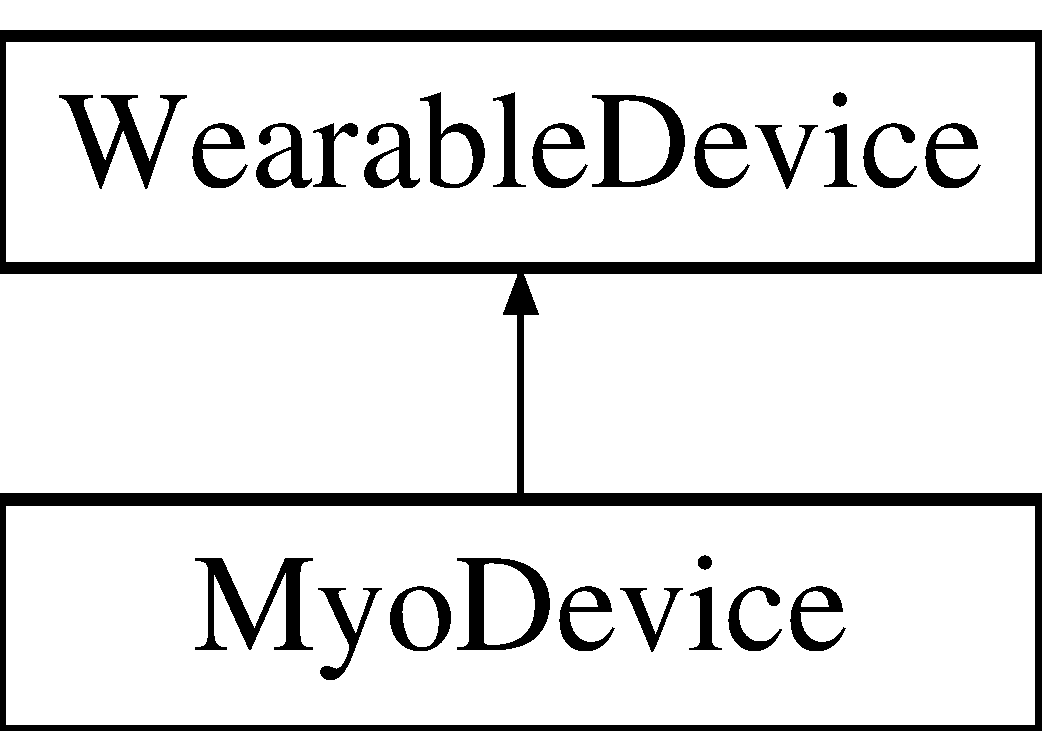
\includegraphics[height=2.000000cm]{class_myo_device}
\end{center}
\end{figure}
\subsection*{Public Member Functions}
\begin{DoxyCompactItemize}
\item 
\hyperlink{class_myo_device_aa6d9def395a5d1704f1734d944a1ab98}{Myo\+Device} (\hyperlink{class_shared_command_data}{Shared\+Command\+Data} $\ast$shared\+Command\+Data, \hyperlink{class_control_state}{Control\+State} $\ast$control\+State, std\+::string application\+Identifier, \hyperlink{class_main_g_u_i}{Main\+G\+U\+I} $\ast$main\+Gui\+Handle, \hyperlink{class_profile_manager}{Profile\+Manager} $\ast$profile\+Manager\+Handle)
\item 
void \hyperlink{class_myo_device_af446081b034056edff7d7132102f1a8c}{set\+Find\+Myo\+Timeout} (unsigned int milliseconds)
\item 
void \hyperlink{class_myo_device_a395ebe609f5ccc11e85a5aa3002dddb7}{set\+Myo\+Event\+Loop\+Duration} (unsigned int milliseconds)
\item 
void \hyperlink{class_myo_device_a263e12e527f3984e8e2946f52d4fa111}{run\+Device\+Loop} ()
\item 
int \hyperlink{class_myo_device_a14db6f7115e407711091beed9b9992a6}{get\+Device\+Error} ()
\item 
void \hyperlink{class_myo_device_a79f6967817e023bca1843028ad3a0329}{update\+Profiles} (void)
\end{DoxyCompactItemize}
\subsection*{Additional Inherited Members}


\subsection{Detailed Description}
Handles the Myo device, collecting the data using the Myo A\+P\+I, and converting the data to keyboard and mouse commands by sending it through a data pipeline. 

\subsection{Constructor \& Destructor Documentation}
\hypertarget{class_myo_device_aa6d9def395a5d1704f1734d944a1ab98}{\index{Myo\+Device@{Myo\+Device}!Myo\+Device@{Myo\+Device}}
\index{Myo\+Device@{Myo\+Device}!Myo\+Device@{Myo\+Device}}
\subsubsection[{Myo\+Device}]{\setlength{\rightskip}{0pt plus 5cm}Myo\+Device\+::\+Myo\+Device (
\begin{DoxyParamCaption}
\item[{{\bf Shared\+Command\+Data} $\ast$}]{shared\+Command\+Data, }
\item[{{\bf Control\+State} $\ast$}]{control\+State, }
\item[{std\+::string}]{application\+Identifier, }
\item[{{\bf Main\+G\+U\+I} $\ast$}]{main\+Gui\+Handle, }
\item[{{\bf Profile\+Manager} $\ast$}]{profile\+Manager\+Handle}
\end{DoxyParamCaption}
)}}\label{class_myo_device_aa6d9def395a5d1704f1734d944a1ab98}
The constructor for the \hyperlink{class_myo_device}{Myo\+Device}.


\begin{DoxyParams}{Parameters}
{\em shared\+Command\+Data} & A handle to the S\+C\+D so that the device can post commands. \\
\hline
{\em control\+State} & A handle to the \hyperlink{class_control_state}{Control\+State} object so that the application state can be changed, and so that the device can read the current state. \\
\hline
{\em application\+Identifier} & A myo-\/specific app identifier used to create the myo hub. \\
\hline
\end{DoxyParams}


\subsection{Member Function Documentation}
\hypertarget{class_myo_device_a14db6f7115e407711091beed9b9992a6}{\index{Myo\+Device@{Myo\+Device}!get\+Device\+Error@{get\+Device\+Error}}
\index{get\+Device\+Error@{get\+Device\+Error}!Myo\+Device@{Myo\+Device}}
\subsubsection[{get\+Device\+Error}]{\setlength{\rightskip}{0pt plus 5cm}int Myo\+Device\+::get\+Device\+Error (
\begin{DoxyParamCaption}
{}
\end{DoxyParamCaption}
)\hspace{0.3cm}{\ttfamily [virtual]}}}\label{class_myo_device_a14db6f7115e407711091beed9b9992a6}
Returns an error code associated with the device, once the device thread has stopped running.

\begin{DoxyReturn}{Returns}
An error code. 
\end{DoxyReturn}


Implements \hyperlink{class_wearable_device_a1c0b4d47e9949bfcfc7111a2615538c0}{Wearable\+Device}.

\hypertarget{class_myo_device_a263e12e527f3984e8e2946f52d4fa111}{\index{Myo\+Device@{Myo\+Device}!run\+Device\+Loop@{run\+Device\+Loop}}
\index{run\+Device\+Loop@{run\+Device\+Loop}!Myo\+Device@{Myo\+Device}}
\subsubsection[{run\+Device\+Loop}]{\setlength{\rightskip}{0pt plus 5cm}void Myo\+Device\+::run\+Device\+Loop (
\begin{DoxyParamCaption}
{}
\end{DoxyParamCaption}
)\hspace{0.3cm}{\ttfamily [virtual]}}}\label{class_myo_device_a263e12e527f3984e8e2946f52d4fa111}
Runs the device loop. This sets up the data pipeline, searches for a Myo device, registers the callback functions, and then enters a loop that waits for events and calls the callback functions. 

Implements \hyperlink{class_wearable_device_a37bf388865b8bcf162e3fe89a23bd3e2}{Wearable\+Device}.

\hypertarget{class_myo_device_af446081b034056edff7d7132102f1a8c}{\index{Myo\+Device@{Myo\+Device}!set\+Find\+Myo\+Timeout@{set\+Find\+Myo\+Timeout}}
\index{set\+Find\+Myo\+Timeout@{set\+Find\+Myo\+Timeout}!Myo\+Device@{Myo\+Device}}
\subsubsection[{set\+Find\+Myo\+Timeout}]{\setlength{\rightskip}{0pt plus 5cm}void Myo\+Device\+::set\+Find\+Myo\+Timeout (
\begin{DoxyParamCaption}
\item[{unsigned int}]{milliseconds}
\end{DoxyParamCaption}
)}}\label{class_myo_device_af446081b034056edff7d7132102f1a8c}
Sets the amount of time that should be spent looking for a Myo device. If a Myo cannot be found within this amount of time, the device thread will exit with an error.


\begin{DoxyParams}{Parameters}
{\em milliseconds} & Number of milliseconds to wait for a Myo. If this is a 0, it will search until one is found (indefinitely). \\
\hline
\end{DoxyParams}
\hypertarget{class_myo_device_a395ebe609f5ccc11e85a5aa3002dddb7}{\index{Myo\+Device@{Myo\+Device}!set\+Myo\+Event\+Loop\+Duration@{set\+Myo\+Event\+Loop\+Duration}}
\index{set\+Myo\+Event\+Loop\+Duration@{set\+Myo\+Event\+Loop\+Duration}!Myo\+Device@{Myo\+Device}}
\subsubsection[{set\+Myo\+Event\+Loop\+Duration}]{\setlength{\rightskip}{0pt plus 5cm}void Myo\+Device\+::set\+Myo\+Event\+Loop\+Duration (
\begin{DoxyParamCaption}
\item[{unsigned int}]{milliseconds}
\end{DoxyParamCaption}
)}}\label{class_myo_device_a395ebe609f5ccc11e85a5aa3002dddb7}
Sets the amount of time, in milliseconds, the Myo event loop should run. While the Myo event loop is running, Midas has no control over the device. The device can only be exited while outside of the Myo event loop.


\begin{DoxyParams}{Parameters}
{\em milliseconds} & Number of milliseconds to stay in the event loop. \\
\hline
\end{DoxyParams}
\hypertarget{class_myo_device_a79f6967817e023bca1843028ad3a0329}{\index{Myo\+Device@{Myo\+Device}!update\+Profiles@{update\+Profiles}}
\index{update\+Profiles@{update\+Profiles}!Myo\+Device@{Myo\+Device}}
\subsubsection[{update\+Profiles}]{\setlength{\rightskip}{0pt plus 5cm}void Myo\+Device\+::update\+Profiles (
\begin{DoxyParamCaption}
\item[{void}]{}
\end{DoxyParamCaption}
)}}\label{class_myo_device_a79f6967817e023bca1843028ad3a0329}
Update filters internal mechanisms if the profile changes.

\begin{DoxyReturn}{Returns}
void. 
\end{DoxyReturn}


The documentation for this class was generated from the following files\+:\begin{DoxyCompactItemize}
\item 
Myo\+Device.\+h\item 
Myo\+Device.\+cpp\end{DoxyCompactItemize}

\hypertarget{class_myo_translation_filter}{\section{Myo\+Translation\+Filter Class Reference}
\label{class_myo_translation_filter}\index{Myo\+Translation\+Filter@{Myo\+Translation\+Filter}}
}


{\ttfamily \#include $<$Myo\+Translation\+Filter.\+h$>$}

Inheritance diagram for Myo\+Translation\+Filter\+:\begin{figure}[H]
\begin{center}
\leavevmode
\includegraphics[height=2.000000cm]{class_myo_translation_filter}
\end{center}
\end{figure}
\subsection*{Public Member Functions}
\begin{DoxyCompactItemize}
\item 
\hyperlink{class_myo_translation_filter_aacbdcc20b57a927b758770e82111ce12}{Myo\+Translation\+Filter} (\hyperlink{class_control_state}{Control\+State} $\ast$control\+State)
\item 
void \hyperlink{class_myo_translation_filter_a9f72c6ac36ed5ea26574db4b207a0597}{process} ()
\item 
filter\+Error \hyperlink{class_myo_translation_filter_a1e1d3d6a3f1bf0d82d17367fc20d704d}{update\+Based\+On\+Profile} (\hyperlink{class_profile_manager}{Profile\+Manager} \&pm, std\+::string name)
\end{DoxyCompactItemize}
\subsection*{Static Public Member Functions}
\begin{DoxyCompactItemize}
\item 
static float \hyperlink{class_myo_translation_filter_a99537f31b135a0378f8b8c335c51941c}{calc\+Ring\+Delta} (float current, float base)
\end{DoxyCompactItemize}
\subsection*{Additional Inherited Members}


\subsection{Detailed Description}
Consult \hyperlink{_filter_8h_source}{Filter.\+h} for concepts regarding Filters. Handles translating from Myo orientation data to mouse movement information. 

\subsection{Constructor \& Destructor Documentation}
\hypertarget{class_myo_translation_filter_aacbdcc20b57a927b758770e82111ce12}{\index{Myo\+Translation\+Filter@{Myo\+Translation\+Filter}!Myo\+Translation\+Filter@{Myo\+Translation\+Filter}}
\index{Myo\+Translation\+Filter@{Myo\+Translation\+Filter}!Myo\+Translation\+Filter@{Myo\+Translation\+Filter}}
\subsubsection[{Myo\+Translation\+Filter}]{\setlength{\rightskip}{0pt plus 5cm}Myo\+Translation\+Filter\+::\+Myo\+Translation\+Filter (
\begin{DoxyParamCaption}
\item[{{\bf Control\+State} $\ast$}]{control\+State}
\end{DoxyParamCaption}
)}}\label{class_myo_translation_filter_aacbdcc20b57a927b758770e82111ce12}
The constructor for \hyperlink{class_myo_translation_filter}{Myo\+Translation\+Filter}.


\begin{DoxyParams}{Parameters}
{\em control\+State} & A handle to \hyperlink{class_control_state}{Control\+State}, to keep track of the application state. \\
\hline
\end{DoxyParams}


\subsection{Member Function Documentation}
\hypertarget{class_myo_translation_filter_a99537f31b135a0378f8b8c335c51941c}{\index{Myo\+Translation\+Filter@{Myo\+Translation\+Filter}!calc\+Ring\+Delta@{calc\+Ring\+Delta}}
\index{calc\+Ring\+Delta@{calc\+Ring\+Delta}!Myo\+Translation\+Filter@{Myo\+Translation\+Filter}}
\subsubsection[{calc\+Ring\+Delta}]{\setlength{\rightskip}{0pt plus 5cm}float Myo\+Translation\+Filter\+::calc\+Ring\+Delta (
\begin{DoxyParamCaption}
\item[{float}]{current, }
\item[{float}]{base}
\end{DoxyParamCaption}
)\hspace{0.3cm}{\ttfamily [static]}}}\label{class_myo_translation_filter_a99537f31b135a0378f8b8c335c51941c}
Calculates the delta (in radians) between a base angle and a current angle, with respect to a ring. The pupose is to ensure that wrapping around the crossover section of the ring has no effect on the output which should safely range from -\/pi to +pi.


\begin{DoxyParams}{Parameters}
{\em current} & The current angle (in radians) that is being compared (from -\/\+Pi to pi rad) \\
\hline
{\em base} & The base angle (in radians) that is being compared against \\
\hline
\end{DoxyParams}
\begin{DoxyReturn}{Returns}
a value from -\/pi to +pi representing the delta between two input angles 
\end{DoxyReturn}
\hypertarget{class_myo_translation_filter_a9f72c6ac36ed5ea26574db4b207a0597}{\index{Myo\+Translation\+Filter@{Myo\+Translation\+Filter}!process@{process}}
\index{process@{process}!Myo\+Translation\+Filter@{Myo\+Translation\+Filter}}
\subsubsection[{process}]{\setlength{\rightskip}{0pt plus 5cm}void Myo\+Translation\+Filter\+::process (
\begin{DoxyParamCaption}
{}
\end{DoxyParamCaption}
)\hspace{0.3cm}{\ttfamily [virtual]}}}\label{class_myo_translation_filter_a9f72c6ac36ed5ea26574db4b207a0597}
Convert the supplied orientation data into mouse movement information, in the form of a percent of the total mouse velocity along both the x and y axes. 

Implements \hyperlink{class_filter_a2f7afde0413c71a3e4947a0537ca8996}{Filter}.

\hypertarget{class_myo_translation_filter_a1e1d3d6a3f1bf0d82d17367fc20d704d}{\index{Myo\+Translation\+Filter@{Myo\+Translation\+Filter}!update\+Based\+On\+Profile@{update\+Based\+On\+Profile}}
\index{update\+Based\+On\+Profile@{update\+Based\+On\+Profile}!Myo\+Translation\+Filter@{Myo\+Translation\+Filter}}
\subsubsection[{update\+Based\+On\+Profile}]{\setlength{\rightskip}{0pt plus 5cm}filter\+Error Myo\+Translation\+Filter\+::update\+Based\+On\+Profile (
\begin{DoxyParamCaption}
\item[{{\bf Profile\+Manager} \&}]{pm, }
\item[{std\+::string}]{name}
\end{DoxyParamCaption}
)\hspace{0.3cm}{\ttfamily [virtual]}}}\label{class_myo_translation_filter_a1e1d3d6a3f1bf0d82d17367fc20d704d}
Update filters internal mechanisms if the profile changes.

\begin{DoxyReturn}{Returns}
The error code of the filter after completion. 
\end{DoxyReturn}


Reimplemented from \hyperlink{class_filter_a9ec2fbdbabb60c91e32048ebe386e372}{Filter}.



The documentation for this class was generated from the following files\+:\begin{DoxyCompactItemize}
\item 
Myo\+Translation\+Filter.\+h\item 
Myo\+Translation\+Filter.\+cpp\end{DoxyCompactItemize}

\hypertarget{structpoint}{\section{point Struct Reference}
\label{structpoint}\index{point@{point}}
}


{\ttfamily \#include $<$Midas\+Common.\+h$>$}

\subsection*{Public Member Functions}
\begin{DoxyCompactItemize}
\item 
\hypertarget{structpoint_a147de248dfeac81bd1c4da13e4ce01b2}{{\bfseries point} (int x\+Val=0, int y\+Val=0)}\label{structpoint_a147de248dfeac81bd1c4da13e4ce01b2}

\end{DoxyCompactItemize}
\subsection*{Public Attributes}
\begin{DoxyCompactItemize}
\item 
\hypertarget{structpoint_ad679b07fb69d55f5ad454d0f1f2891d5}{int {\bfseries x}}\label{structpoint_ad679b07fb69d55f5ad454d0f1f2891d5}

\item 
\hypertarget{structpoint_a9a82ca9504acabb1e30569f89c805471}{int {\bfseries y}}\label{structpoint_a9a82ca9504acabb1e30569f89c805471}

\end{DoxyCompactItemize}


\subsection{Detailed Description}
A simple point consisting of two coordinates, x and y. 

The documentation for this struct was generated from the following file\+:\begin{DoxyCompactItemize}
\item 
Midas\+Common.\+h\end{DoxyCompactItemize}

\hypertarget{class_pose_displayer}{\section{Pose\+Displayer Class Reference}
\label{class_pose_displayer}\index{Pose\+Displayer@{Pose\+Displayer}}
}
Inheritance diagram for Pose\+Displayer\+:\begin{figure}[H]
\begin{center}
\leavevmode
\includegraphics[height=2.000000cm]{class_pose_displayer}
\end{center}
\end{figure}
\subsection*{Public Slots}
\begin{DoxyCompactItemize}
\item 
\hypertarget{class_pose_displayer_aecd22b32ac50bd85ae85b230a170aa40}{void {\bfseries handle\+Pose\+Images} (std\+::vector$<$ \hyperlink{structsequence_image_set}{sequence\+Image\+Set} $>$ pose\+Images)}\label{class_pose_displayer_aecd22b32ac50bd85ae85b230a170aa40}

\end{DoxyCompactItemize}
\subsection*{Public Member Functions}
\begin{DoxyCompactItemize}
\item 
\hypertarget{class_pose_displayer_a4336244149931fcc4d83974e5ef79188}{{\bfseries Pose\+Displayer} (int widget\+Width, int widget\+Height, Q\+Widget $\ast$parent=0)}\label{class_pose_displayer_a4336244149931fcc4d83974e5ef79188}

\item 
\hypertarget{class_pose_displayer_aa6a9f27ba7e55f8337da42e290a3810e}{Q\+Size {\bfseries size\+Hint} () const }\label{class_pose_displayer_aa6a9f27ba7e55f8337da42e290a3810e}

\end{DoxyCompactItemize}
\subsection*{Protected Member Functions}
\begin{DoxyCompactItemize}
\item 
\hypertarget{class_pose_displayer_a12016e6a8a03bee7264f5bdad4f4501d}{void {\bfseries resize\+Event} (Q\+Resize\+Event $\ast$event)}\label{class_pose_displayer_a12016e6a8a03bee7264f5bdad4f4501d}

\end{DoxyCompactItemize}


The documentation for this class was generated from the following files\+:\begin{DoxyCompactItemize}
\item 
Pose\+Displayer.\+h\item 
Pose\+Displayer.\+cpp\end{DoxyCompactItemize}

\hypertarget{structprofile}{\section{profile Struct Reference}
\label{structprofile}\index{profile@{profile}}
}
\subsection*{Public Attributes}
\begin{DoxyCompactItemize}
\item 
\hypertarget{structprofile_ae5a8115d37d3527b7b20b2b90a5cdaa3}{std\+::string {\bfseries profile\+Name}}\label{structprofile_ae5a8115d37d3527b7b20b2b90a5cdaa3}

\item 
\hypertarget{structprofile_a92cf53f4df6b3e1a1f82f1c020e1049f}{std\+::vector$<$ \hyperlink{structprofile_sequence}{profile\+Sequence} $>$ {\bfseries profile\+Sequences}}\label{structprofile_a92cf53f4df6b3e1a1f82f1c020e1049f}

\item 
\hypertarget{structprofile_af0260fc43229728101d5db86884f54a0}{std\+::vector$<$ \hyperlink{structhold}{hold} $>$ {\bfseries holds}}\label{structprofile_af0260fc43229728101d5db86884f54a0}

\end{DoxyCompactItemize}


The documentation for this struct was generated from the following file\+:\begin{DoxyCompactItemize}
\item 
Profile\+Manager.\+h\end{DoxyCompactItemize}

\hypertarget{class_profile_displayer}{\section{Profile\+Displayer Class Reference}
\label{class_profile_displayer}\index{Profile\+Displayer@{Profile\+Displayer}}
}
Inheritance diagram for Profile\+Displayer\+:\begin{figure}[H]
\begin{center}
\leavevmode
\includegraphics[height=2.000000cm]{class_profile_displayer}
\end{center}
\end{figure}
\subsection*{Signals}
\begin{DoxyCompactItemize}
\item 
\hypertarget{class_profile_displayer_af486a2acd152399dfe9c4a3b326ead13}{void {\bfseries emit\+Change\+Profile} (Q\+String)}\label{class_profile_displayer_af486a2acd152399dfe9c4a3b326ead13}

\end{DoxyCompactItemize}
\subsection*{Public Member Functions}
\begin{DoxyCompactItemize}
\item 
\hypertarget{class_profile_displayer_a0a9cf5e9b09969f8031e4c4407deadd0}{{\bfseries Profile\+Displayer} (std\+::string name, int widget\+Width=P\+R\+O\+F\+\_\+\+I\+N\+D\+I\+C\+A\+T\+O\+R\+\_\+\+W\+I\+D\+T\+H, int widget\+Height=P\+R\+O\+F\+\_\+\+I\+N\+D\+I\+C\+A\+T\+O\+R\+\_\+\+H\+E\+I\+G\+H\+T, Q\+Widget $\ast$parent=0)}\label{class_profile_displayer_a0a9cf5e9b09969f8031e4c4407deadd0}

\item 
\hypertarget{class_profile_displayer_a8b66497d9c3add926298e5657d0b0d56}{Q\+Size {\bfseries size\+Hint} () const }\label{class_profile_displayer_a8b66497d9c3add926298e5657d0b0d56}

\end{DoxyCompactItemize}
\subsection*{Protected Member Functions}
\begin{DoxyCompactItemize}
\item 
virtual void \hyperlink{class_profile_displayer_a193f7ee781f7f22163253a98ce5ca32f}{mouse\+Press\+Event} (Q\+Mouse\+Event $\ast$event)
\item 
virtual void \hyperlink{class_profile_displayer_a23a01012f4cb4121e0de68ff846e1324}{mouse\+Release\+Event} (Q\+Mouse\+Event $\ast$event)
\item 
\hypertarget{class_profile_displayer_a9f751256b3af226c87522841f4c02d04}{virtual void {\bfseries mouse\+Move\+Event} (Q\+Mouse\+Event $\ast$event)}\label{class_profile_displayer_a9f751256b3af226c87522841f4c02d04}

\end{DoxyCompactItemize}


\subsection{Member Function Documentation}
\hypertarget{class_profile_displayer_a193f7ee781f7f22163253a98ce5ca32f}{\index{Profile\+Displayer@{Profile\+Displayer}!mouse\+Press\+Event@{mouse\+Press\+Event}}
\index{mouse\+Press\+Event@{mouse\+Press\+Event}!Profile\+Displayer@{Profile\+Displayer}}
\subsubsection[{mouse\+Press\+Event}]{\setlength{\rightskip}{0pt plus 5cm}void Profile\+Displayer\+::mouse\+Press\+Event (
\begin{DoxyParamCaption}
\item[{Q\+Mouse\+Event $\ast$}]{event}
\end{DoxyParamCaption}
)\hspace{0.3cm}{\ttfamily [protected]}, {\ttfamily [virtual]}}}\label{class_profile_displayer_a193f7ee781f7f22163253a98ce5ca32f}
The event handler function that is called when the widget is clicked on by the mouse.


\begin{DoxyParams}{Parameters}
{\em event} & The mouse event structure, with information about the mouse press. \\
\hline
\end{DoxyParams}
\hypertarget{class_profile_displayer_a23a01012f4cb4121e0de68ff846e1324}{\index{Profile\+Displayer@{Profile\+Displayer}!mouse\+Release\+Event@{mouse\+Release\+Event}}
\index{mouse\+Release\+Event@{mouse\+Release\+Event}!Profile\+Displayer@{Profile\+Displayer}}
\subsubsection[{mouse\+Release\+Event}]{\setlength{\rightskip}{0pt plus 5cm}void Profile\+Displayer\+::mouse\+Release\+Event (
\begin{DoxyParamCaption}
\item[{Q\+Mouse\+Event $\ast$}]{event}
\end{DoxyParamCaption}
)\hspace{0.3cm}{\ttfamily [protected]}, {\ttfamily [virtual]}}}\label{class_profile_displayer_a23a01012f4cb4121e0de68ff846e1324}
The event handler function that is called when the widget is released by the mouse.


\begin{DoxyParams}{Parameters}
{\em event} & The mouse event structure, with information about the mouse release. \\
\hline
\end{DoxyParams}


The documentation for this class was generated from the following files\+:\begin{DoxyCompactItemize}
\item 
Profile\+Displayer.\+h\item 
Profile\+Displayer.\+cpp\end{DoxyCompactItemize}

\hypertarget{class_profile_manager}{\section{Profile\+Manager Class Reference}
\label{class_profile_manager}\index{Profile\+Manager@{Profile\+Manager}}
}
\subsection*{Public Member Functions}
\begin{DoxyCompactItemize}
\item 
\hypertarget{class_profile_manager_a2465a14f4a641d033efafad1b6386543}{void {\bfseries load\+Profiles\+From\+File} (std\+::string file\+Name)}\label{class_profile_manager_a2465a14f4a641d033efafad1b6386543}

\item 
\hypertarget{class_profile_manager_a2ddbbea97ffb2c2b577d360b3c54112f}{std\+::vector$<$ \hyperlink{structprofile}{profile} $>$ $\ast$ {\bfseries get\+Profiles} ()}\label{class_profile_manager_a2ddbbea97ffb2c2b577d360b3c54112f}

\end{DoxyCompactItemize}


The documentation for this class was generated from the following files\+:\begin{DoxyCompactItemize}
\item 
Profile\+Manager.\+h\item 
Profile\+Manager.\+cpp\end{DoxyCompactItemize}

\hypertarget{structprofile_sequence}{\section{profile\+Sequence Struct Reference}
\label{structprofile_sequence}\index{profile\+Sequence@{profile\+Sequence}}
}
\subsection*{Public Attributes}
\begin{DoxyCompactItemize}
\item 
\hypertarget{structprofile_sequence_a7340db9d07b24cfce971ea637118d17d}{std\+::string {\bfseries state}}\label{structprofile_sequence_a7340db9d07b24cfce971ea637118d17d}

\item 
\hypertarget{structprofile_sequence_aa86a426828d07da3dd96e7989c709f3d}{std\+::string {\bfseries name}}\label{structprofile_sequence_aa86a426828d07da3dd96e7989c709f3d}

\item 
\hypertarget{structprofile_sequence_ad663fa61f1ba1ee143b19c3154fa99d9}{std\+::vector$<$ \hyperlink{structgesture}{gesture} $>$ {\bfseries gestures}}\label{structprofile_sequence_ad663fa61f1ba1ee143b19c3154fa99d9}

\item 
\hypertarget{structprofile_sequence_aa108287acf821469291f50a378827416}{\hyperlink{structcommand}{command} {\bfseries cmd}}\label{structprofile_sequence_aa108287acf821469291f50a378827416}

\end{DoxyCompactItemize}


The documentation for this struct was generated from the following file\+:\begin{DoxyCompactItemize}
\item 
Profile\+Manager.\+h\end{DoxyCompactItemize}

\hypertarget{class_profile_signaller}{\section{Profile\+Signaller Class Reference}
\label{class_profile_signaller}\index{Profile\+Signaller@{Profile\+Signaller}}
}
Inheritance diagram for Profile\+Signaller\+:\begin{figure}[H]
\begin{center}
\leavevmode
\includegraphics[height=2.000000cm]{class_profile_signaller}
\end{center}
\end{figure}
\subsection*{Public Slots}
\begin{DoxyCompactItemize}
\item 
\hypertarget{class_profile_signaller_a8e4416a01b54b90ebd7dcf749af7df33}{void {\bfseries handle\+Profile\+Press} (Q\+String)}\label{class_profile_signaller_a8e4416a01b54b90ebd7dcf749af7df33}

\end{DoxyCompactItemize}
\subsection*{Public Member Functions}
\begin{DoxyCompactItemize}
\item 
\hypertarget{class_profile_signaller_ae062c8a3a74c6db214aef6bbe4047781}{{\bfseries Profile\+Signaller} (Q\+Object $\ast$parent=0)}\label{class_profile_signaller_ae062c8a3a74c6db214aef6bbe4047781}

\item 
\hypertarget{class_profile_signaller_aca2c0e1b5eb9488544fa2a9e9a1dd411}{std\+::string {\bfseries get\+Profile\+Name} ()}\label{class_profile_signaller_aca2c0e1b5eb9488544fa2a9e9a1dd411}

\end{DoxyCompactItemize}


The documentation for this class was generated from the following files\+:\begin{DoxyCompactItemize}
\item 
Profile\+Signaller.\+h\item 
Profile\+Signaller.\+cpp\end{DoxyCompactItemize}

\hypertarget{classring_data}{\section{ring\+Data Class Reference}
\label{classring_data}\index{ring\+Data@{ring\+Data}}
}
\subsection*{Classes}
\begin{DoxyCompactItemize}
\item 
struct \hyperlink{structring_data_1_1keyboard_value}{keyboard\+Value}
\end{DoxyCompactItemize}
\subsection*{Public Member Functions}
\begin{DoxyCompactItemize}
\item 
\hypertarget{classring_data_a8dea49491667b4201d598d58c17b64c4}{{\bfseries ring\+Data} (const \hyperlink{classring_data}{ring\+Data} \&rd)}\label{classring_data_a8dea49491667b4201d598d58c17b64c4}

\item 
\hypertarget{classring_data_af7fd6fa0c88824db516159f43d840f05}{std\+::vector$<$ \hyperlink{structring_data_1_1keyboard_value}{keyboard\+Value} $>$ $\ast$ {\bfseries get\+Ring\+In\+Vector\+Handle} ()}\label{classring_data_af7fd6fa0c88824db516159f43d840f05}

\item 
\hypertarget{classring_data_ae0a8b742358271e92a4bfcad11bbb197}{std\+::vector$<$ \hyperlink{structring_data_1_1keyboard_value}{keyboard\+Value} $>$ $\ast$ {\bfseries get\+Ring\+Out\+Vector\+Handle} ()}\label{classring_data_ae0a8b742358271e92a4bfcad11bbb197}

\item 
\hypertarget{classring_data_a189c1244a8472ebaf7e9e24a9d2465d4}{void {\bfseries set\+Ring\+In\+Vector} (std\+::vector$<$ \hyperlink{structring_data_1_1keyboard_value}{keyboard\+Value} $>$ ring\+In\+Val)}\label{classring_data_a189c1244a8472ebaf7e9e24a9d2465d4}

\item 
\hypertarget{classring_data_ae46cf7c208005f9be4e21c84a00b8d8a}{void {\bfseries set\+Ring\+Out\+Vector} (std\+::vector$<$ \hyperlink{structring_data_1_1keyboard_value}{keyboard\+Value} $>$ ring\+Out\+Val)}\label{classring_data_ae46cf7c208005f9be4e21c84a00b8d8a}

\end{DoxyCompactItemize}


The documentation for this class was generated from the following files\+:\begin{DoxyCompactItemize}
\item 
Ring\+Data.\+h\item 
Ring\+Data.\+cpp\end{DoxyCompactItemize}

\hypertarget{class_s_c_d_digester}{\section{S\+C\+D\+Digester Class Reference}
\label{class_s_c_d_digester}\index{S\+C\+D\+Digester@{S\+C\+D\+Digester}}
}
\subsection*{Public Member Functions}
\begin{DoxyCompactItemize}
\item 
\hypertarget{class_s_c_d_digester_a0c44bfc57617bcf2cebd469b3ced85ad}{{\bfseries S\+C\+D\+Digester} (\hyperlink{class_shared_command_data}{Shared\+Command\+Data} $\ast$scd, \hyperlink{class_midas_thread}{Midas\+Thread} $\ast$thread, \hyperlink{class_control_state}{Control\+State} $\ast$cntrl\+State\+Handle, \hyperlink{class_mouse_ctrl}{Mouse\+Ctrl} $\ast$mouse\+Ctrl, \hyperlink{class_kybrd_ctrl}{Kybrd\+Ctrl} $\ast$kybrd\+Ctrl, std\+::vector$<$ \hyperlink{classring_data}{ring\+Data} $>$ $\ast$kybrd\+Ring\+Data)}\label{class_s_c_d_digester_a0c44bfc57617bcf2cebd469b3ced85ad}

\item 
\hypertarget{class_s_c_d_digester_a799635f57efa9954cdbe3fae86f33313}{void {\bfseries digest} ()}\label{class_s_c_d_digester_a799635f57efa9954cdbe3fae86f33313}

\end{DoxyCompactItemize}


The documentation for this class was generated from the following files\+:\begin{DoxyCompactItemize}
\item 
S\+C\+D\+Digester.\+h\item 
S\+C\+D\+Digester.\+cpp\end{DoxyCompactItemize}

\hypertarget{struct_seq_element}{\section{Seq\+Element Struct Reference}
\label{struct_seq_element}\index{Seq\+Element@{Seq\+Element}}
}
\subsection*{Public Types}
\begin{DoxyCompactItemize}
\item 
\hypertarget{struct_seq_element_ac3921567c5f16b22cc77a0944f5bf330}{enum {\bfseries Pose\+Length} \{ {\bfseries T\+A\+P}, 
{\bfseries H\+O\+L\+D}, 
{\bfseries I\+M\+M\+E\+D\+I\+A\+T\+E}
 \}}\label{struct_seq_element_ac3921567c5f16b22cc77a0944f5bf330}

\end{DoxyCompactItemize}
\subsection*{Public Member Functions}
\begin{DoxyCompactItemize}
\item 
\hypertarget{struct_seq_element_ae967d4b0e39f9e0a0b0b83dac35b49fb}{{\bfseries Seq\+Element} (Pose\+::\+Type type)}\label{struct_seq_element_ae967d4b0e39f9e0a0b0b83dac35b49fb}

\item 
\hypertarget{struct_seq_element_a5bd19468f7c218fe9956dc2ee60d96a4}{{\bfseries Seq\+Element} (Pose\+::\+Type type, Pose\+Length P\+L)}\label{struct_seq_element_a5bd19468f7c218fe9956dc2ee60d96a4}

\item 
\hypertarget{struct_seq_element_a5dbbd23498ab1d1910d2c05787c4f44a}{bool {\bfseries operator==} (\hyperlink{struct_seq_element}{Seq\+Element} \&e)}\label{struct_seq_element_a5dbbd23498ab1d1910d2c05787c4f44a}

\item 
\hypertarget{struct_seq_element_a800eb0b2ad54ae37313733e8bcb15e71}{bool {\bfseries operator!=} (\hyperlink{struct_seq_element}{Seq\+Element} \&e)}\label{struct_seq_element_a800eb0b2ad54ae37313733e8bcb15e71}

\end{DoxyCompactItemize}
\subsection*{Public Attributes}
\begin{DoxyCompactItemize}
\item 
\hypertarget{struct_seq_element_a0ffe18c62f22e5bb8147bfbffd0a928a}{Pose\+::\+Type {\bfseries type}}\label{struct_seq_element_a0ffe18c62f22e5bb8147bfbffd0a928a}

\item 
\hypertarget{struct_seq_element_acffc29093e5d1452d773435890e94688}{Pose\+Length {\bfseries pose\+Len} = Pose\+Length\+::\+T\+A\+P}\label{struct_seq_element_acffc29093e5d1452d773435890e94688}

\end{DoxyCompactItemize}


The documentation for this struct was generated from the following file\+:\begin{DoxyCompactItemize}
\item 
Myo\+Common.\+h\end{DoxyCompactItemize}

\hypertarget{structsequence_data}{\section{sequence\+Data Struct Reference}
\label{structsequence_data}\index{sequence\+Data@{sequence\+Data}}
}
\subsection*{Public Attributes}
\begin{DoxyCompactItemize}
\item 
\hypertarget{structsequence_data_a2c1a2ac21a0d7dd02848765d10b4cba3}{Q\+Label $\ast$ {\bfseries seq\+Label}}\label{structsequence_data_a2c1a2ac21a0d7dd02848765d10b4cba3}

\item 
\hypertarget{structsequence_data_ad3c34c1b6cd3bc35fb2c1bc927d4c382}{Q\+Label $\ast$ {\bfseries seq\+Pos\+Label}}\label{structsequence_data_ad3c34c1b6cd3bc35fb2c1bc927d4c382}

\item 
\hypertarget{structsequence_data_a95768a03bf6b9968437b2bcd79e5e44a}{int {\bfseries image\+Offset}}\label{structsequence_data_a95768a03bf6b9968437b2bcd79e5e44a}

\item 
\hypertarget{structsequence_data_a5ddb69cc1337741e51e7028eb34df87f}{std\+::vector$<$ \hyperlink{structsequence_image_set}{sequence\+Image\+Set} $>$ {\bfseries sequence\+Images}}\label{structsequence_data_a5ddb69cc1337741e51e7028eb34df87f}

\end{DoxyCompactItemize}


The documentation for this struct was generated from the following file\+:\begin{DoxyCompactItemize}
\item 
Myo\+Common.\+h\end{DoxyCompactItemize}

\hypertarget{class_sequence_displayer}{\section{Sequence\+Displayer Class Reference}
\label{class_sequence_displayer}\index{Sequence\+Displayer@{Sequence\+Displayer}}
}


{\ttfamily \#include $<$Sequence\+Displayer.\+h$>$}

Inheritance diagram for Sequence\+Displayer\+:\begin{figure}[H]
\begin{center}
\leavevmode
\includegraphics[height=2.000000cm]{class_sequence_displayer}
\end{center}
\end{figure}
\subsection*{Public Slots}
\begin{DoxyCompactItemize}
\item 
void \hyperlink{class_sequence_displayer_afcc86a900cb5bf28e1b3e6a09d6abeed}{register\+Sequence\+Images} (int, Q\+String, std\+::vector$<$ \hyperlink{structsequence_image_set}{sequence\+Image\+Set} $>$)
\item 
void \hyperlink{class_sequence_displayer_a78aa2211e005356237805dea967d8dda}{show\+Sequences} (std\+::vector$<$ \hyperlink{structsequence_progress_data}{sequence\+Progress\+Data} $>$)
\end{DoxyCompactItemize}
\subsection*{Public Member Functions}
\begin{DoxyCompactItemize}
\item 
\hyperlink{class_sequence_displayer_aa5f4a391a77a9b208ed0a075515ce554}{Sequence\+Displayer} (Q\+Widget $\ast$parent=0)
\item 
Q\+Size \hyperlink{class_sequence_displayer_ab8cad0c7ce49e97ed75af555b5e04556}{size\+Hint} () const 
\end{DoxyCompactItemize}


\subsection{Detailed Description}
The \hyperlink{class_sequence_displayer}{Sequence\+Displayer} class represents a G\+U\+I that can display Midas gesture sequences. These gesture sequences are made up of a series of images that should convey information to the user on what gesture they must perform next in the sequence. 

\subsection{Constructor \& Destructor Documentation}
\hypertarget{class_sequence_displayer_aa5f4a391a77a9b208ed0a075515ce554}{\index{Sequence\+Displayer@{Sequence\+Displayer}!Sequence\+Displayer@{Sequence\+Displayer}}
\index{Sequence\+Displayer@{Sequence\+Displayer}!Sequence\+Displayer@{Sequence\+Displayer}}
\subsubsection[{Sequence\+Displayer}]{\setlength{\rightskip}{0pt plus 5cm}Sequence\+Displayer\+::\+Sequence\+Displayer (
\begin{DoxyParamCaption}
\item[{Q\+Widget $\ast$}]{parent = {\ttfamily 0}}
\end{DoxyParamCaption}
)}}\label{class_sequence_displayer_aa5f4a391a77a9b208ed0a075515ce554}
Constructor for the \hyperlink{class_sequence_displayer}{Sequence\+Displayer}.


\begin{DoxyParams}{Parameters}
{\em parent} & The parent widget. \\
\hline
\end{DoxyParams}


\subsection{Member Function Documentation}
\hypertarget{class_sequence_displayer_afcc86a900cb5bf28e1b3e6a09d6abeed}{\index{Sequence\+Displayer@{Sequence\+Displayer}!register\+Sequence\+Images@{register\+Sequence\+Images}}
\index{register\+Sequence\+Images@{register\+Sequence\+Images}!Sequence\+Displayer@{Sequence\+Displayer}}
\subsubsection[{register\+Sequence\+Images}]{\setlength{\rightskip}{0pt plus 5cm}void Sequence\+Displayer\+::register\+Sequence\+Images (
\begin{DoxyParamCaption}
\item[{int}]{seq\+Id, }
\item[{Q\+String}]{sequence\+Name, }
\item[{std\+::vector$<$ {\bf sequence\+Image\+Set} $>$}]{sequence\+Images}
\end{DoxyParamCaption}
)\hspace{0.3cm}{\ttfamily [slot]}}}\label{class_sequence_displayer_afcc86a900cb5bf28e1b3e6a09d6abeed}
Register a sequence, with an I\+D, name, and set of images.


\begin{DoxyParams}{Parameters}
{\em id} & The id of the sequence. \\
\hline
{\em name} & A human-\/readable name for the sequence. \\
\hline
{\em images} & The images that make up the sequence. Each element of the vector contains two images. \\
\hline
\end{DoxyParams}
\hypertarget{class_sequence_displayer_a78aa2211e005356237805dea967d8dda}{\index{Sequence\+Displayer@{Sequence\+Displayer}!show\+Sequences@{show\+Sequences}}
\index{show\+Sequences@{show\+Sequences}!Sequence\+Displayer@{Sequence\+Displayer}}
\subsubsection[{show\+Sequences}]{\setlength{\rightskip}{0pt plus 5cm}void Sequence\+Displayer\+::show\+Sequences (
\begin{DoxyParamCaption}
\item[{std\+::vector$<$ {\bf sequence\+Progress\+Data} $>$}]{progress\+Pairs}
\end{DoxyParamCaption}
)\hspace{0.3cm}{\ttfamily [slot]}}}\label{class_sequence_displayer_a78aa2211e005356237805dea967d8dda}
Show the provided sequences on the display. The caller supplied a vector of pairs; each pair has a sequence I\+D and a number that represents the current position in the sequence.


\begin{DoxyParams}{Parameters}
{\em sequence\+Id\+Progress\+Pairs} & A vector containing the pairs of sequence I\+Ds and sequence positions. \\
\hline
\end{DoxyParams}
\hypertarget{class_sequence_displayer_ab8cad0c7ce49e97ed75af555b5e04556}{\index{Sequence\+Displayer@{Sequence\+Displayer}!size\+Hint@{size\+Hint}}
\index{size\+Hint@{size\+Hint}!Sequence\+Displayer@{Sequence\+Displayer}}
\subsubsection[{size\+Hint}]{\setlength{\rightskip}{0pt plus 5cm}Q\+Size Sequence\+Displayer\+::size\+Hint (
\begin{DoxyParamCaption}
{}
\end{DoxyParamCaption}
) const}}\label{class_sequence_displayer_ab8cad0c7ce49e97ed75af555b5e04556}
Returns the recommended size of the widget.

\begin{DoxyReturn}{Returns}
The recommended size of the widget. 
\end{DoxyReturn}


The documentation for this class was generated from the following files\+:\begin{DoxyCompactItemize}
\item 
Sequence\+Displayer.\+h\item 
Sequence\+Displayer.\+cpp\end{DoxyCompactItemize}

\hypertarget{class_sequence_image_manager}{\section{Sequence\+Image\+Manager Class Reference}
\label{class_sequence_image_manager}\index{Sequence\+Image\+Manager@{Sequence\+Image\+Manager}}
}
\subsection*{Public Member Functions}
\begin{DoxyCompactItemize}
\item 
\hypertarget{class_sequence_image_manager_a17f2b17310200752af0b8f7ac7a7d775}{void {\bfseries load\+Images} ()}\label{class_sequence_image_manager_a17f2b17310200752af0b8f7ac7a7d775}

\item 
\hypertarget{class_sequence_image_manager_a44a93f8777f6ad8632e85a3db0850e20}{std\+::vector$<$ \hyperlink{structsequence_image_set}{sequence\+Image\+Set} $>$ {\bfseries form\+Sequence\+Set\+From\+Ids} (std\+::vector$<$ int $>$ ids)}\label{class_sequence_image_manager_a44a93f8777f6ad8632e85a3db0850e20}

\end{DoxyCompactItemize}


The documentation for this class was generated from the following files\+:\begin{DoxyCompactItemize}
\item 
Sequence\+Image\+Manager.\+h\item 
Sequence\+Image\+Manager.\+cpp\end{DoxyCompactItemize}

\hypertarget{structsequence_image_set}{\section{sequence\+Image\+Set Struct Reference}
\label{structsequence_image_set}\index{sequence\+Image\+Set@{sequence\+Image\+Set}}
}
\subsection*{Public Attributes}
\begin{DoxyCompactItemize}
\item 
\hypertarget{structsequence_image_set_abcb1e93d769c0353b752e30d2a75deaf}{Q\+Pixmap {\bfseries next\+Image}}\label{structsequence_image_set_abcb1e93d769c0353b752e30d2a75deaf}

\item 
\hypertarget{structsequence_image_set_a48e058ec9aacdd0303b29933f8f062e0}{Q\+Pixmap {\bfseries later\+Image}}\label{structsequence_image_set_a48e058ec9aacdd0303b29933f8f062e0}

\item 
\hypertarget{structsequence_image_set_a1c97e80abacb5bd9105a3afa1eb7832d}{Q\+Label $\ast$ {\bfseries current\+Img\+Label}}\label{structsequence_image_set_a1c97e80abacb5bd9105a3afa1eb7832d}

\item 
\hypertarget{structsequence_image_set_a35a9e791cf30bf489ffbe3a47d6dd32b}{int {\bfseries action\+Tag}}\label{structsequence_image_set_a35a9e791cf30bf489ffbe3a47d6dd32b}

\end{DoxyCompactItemize}


The documentation for this struct was generated from the following file\+:\begin{DoxyCompactItemize}
\item 
Myo\+Common.\+h\end{DoxyCompactItemize}

\hypertarget{structsequence_info}{\section{sequence\+Info Struct Reference}
\label{structsequence_info}\index{sequence\+Info@{sequence\+Info}}
}


{\ttfamily \#include $<$Gesture\+Seq\+Recorder.\+h$>$}

\subsection*{Public Attributes}
\begin{DoxyCompactItemize}
\item 
\hypertarget{structsequence_info_a50d6a6f2a36550816b9cc9bd507b72dc}{sequence {\bfseries seq}}\label{structsequence_info_a50d6a6f2a36550816b9cc9bd507b72dc}

\item 
\hypertarget{structsequence_info_a19a0599ecce102bd084becb5c5cebc75}{\hyperlink{structcommand_data}{command\+Data} {\bfseries sequence\+Response}}\label{structsequence_info_a19a0599ecce102bd084becb5c5cebc75}

\item 
\hypertarget{structsequence_info_a956782dc439d9305d4cf778f6e3aabef}{unsigned int {\bfseries progress}}\label{structsequence_info_a956782dc439d9305d4cf778f6e3aabef}

\item 
\hypertarget{structsequence_info_a361998ebf769619165f8e262ec46233a}{unsigned int {\bfseries id}}\label{structsequence_info_a361998ebf769619165f8e262ec46233a}

\item 
\hypertarget{structsequence_info_a2aae3803a2fabf36bf6fcb174f56f141}{std\+::string {\bfseries sequence\+Name}}\label{structsequence_info_a2aae3803a2fabf36bf6fcb174f56f141}

\end{DoxyCompactItemize}
\subsection*{Static Public Attributes}
\begin{DoxyCompactItemize}
\item 
\hypertarget{structsequence_info_a64458418e842fa396749afba2be7d30b}{static unsigned int {\bfseries counter} = 0}\label{structsequence_info_a64458418e842fa396749afba2be7d30b}

\end{DoxyCompactItemize}


\subsection{Detailed Description}
Wrapper to tie state information to a sequence response. 

The documentation for this struct was generated from the following files\+:\begin{DoxyCompactItemize}
\item 
Gesture\+Seq\+Recorder.\+h\item 
Gesture\+Seq\+Recorder.\+cpp\end{DoxyCompactItemize}

\hypertarget{structsequence_progress_data}{\section{sequence\+Progress\+Data Struct Reference}
\label{structsequence_progress_data}\index{sequence\+Progress\+Data@{sequence\+Progress\+Data}}
}
\subsection*{Public Member Functions}
\begin{DoxyCompactItemize}
\item 
\hypertarget{structsequence_progress_data_aff3ad5730a32774f1ba123b5df847b41}{{\bfseries sequence\+Progress\+Data} (int id, int prog)}\label{structsequence_progress_data_aff3ad5730a32774f1ba123b5df847b41}

\end{DoxyCompactItemize}
\subsection*{Public Attributes}
\begin{DoxyCompactItemize}
\item 
\hypertarget{structsequence_progress_data_a3692ee9b7a74dadaaa6efdc65113b70c}{int {\bfseries seq\+Id}}\label{structsequence_progress_data_a3692ee9b7a74dadaaa6efdc65113b70c}

\item 
\hypertarget{structsequence_progress_data_a4c144a4db3f71c86845962239c3f61b3}{int {\bfseries progress}}\label{structsequence_progress_data_a4c144a4db3f71c86845962239c3f61b3}

\end{DoxyCompactItemize}


The documentation for this struct was generated from the following file\+:\begin{DoxyCompactItemize}
\item 
Myo\+Common.\+h\end{DoxyCompactItemize}

\hypertarget{class_shared_command_data}{\section{Shared\+Command\+Data Class Reference}
\label{class_shared_command_data}\index{Shared\+Command\+Data@{Shared\+Command\+Data}}
}


{\ttfamily \#include $<$Shared\+Command\+Data.\+h$>$}

Inheritance diagram for Shared\+Command\+Data\+:\begin{figure}[H]
\begin{center}
\leavevmode
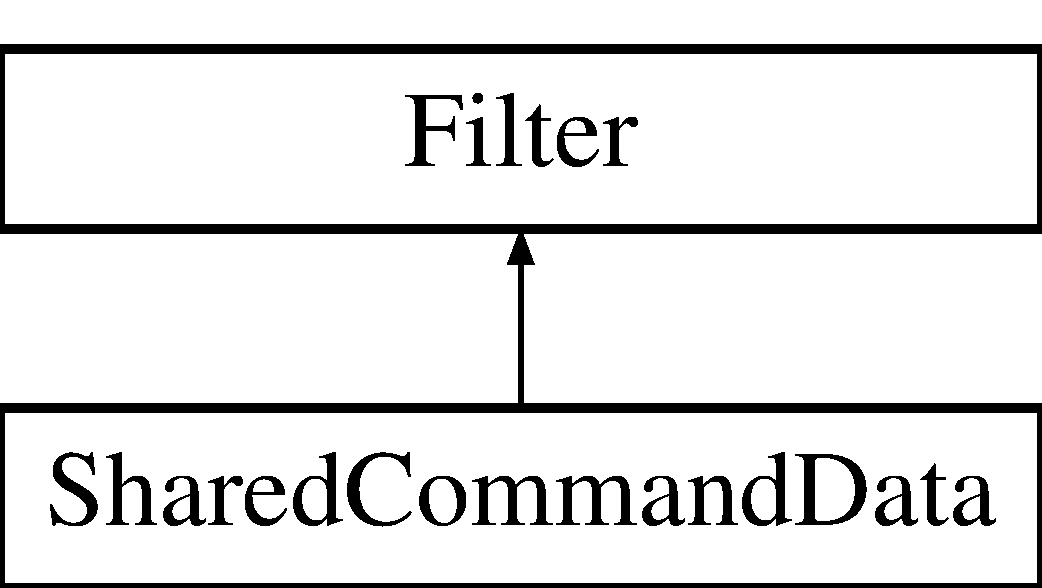
\includegraphics[height=2.000000cm]{class_shared_command_data}
\end{center}
\end{figure}
\subsection*{Public Member Functions}
\begin{DoxyCompactItemize}
\item 
\hypertarget{class_shared_command_data_a3923aef67267c3f32ba84a458f56a8d5}{{\bfseries Shared\+Command\+Data} (unsigned int max\+Kybd\+Gui\+Sel)}\label{class_shared_command_data_a3923aef67267c3f32ba84a458f56a8d5}

\item 
void \hyperlink{class_shared_command_data_a7c2de829c0cd0243e65070df13e1ec73}{add\+Command} (\hyperlink{structcommand_data}{command\+Data} dat)
\item 
bool \hyperlink{class_shared_command_data_a468e88e90b272c6eed02e93a390f5ee4}{try\+Add\+Command} (\hyperlink{structcommand_data}{command\+Data} dat)
\item 
bool \hyperlink{class_shared_command_data_a4da8ee2c7461ec2b67343b6f2e63f70a}{consume\+Command} (\hyperlink{structcommand_data}{command\+Data} \&dat)
\item 
bool \hyperlink{class_shared_command_data_a6c865acfe805a27cd6c052a58168b7d5}{try\+Consume\+Command} (\hyperlink{structcommand_data}{command\+Data} \&out\+Command\+Data)
\item 
void \hyperlink{class_shared_command_data_a8c130b9d388e0f3a13502eb8e3883cbc}{set\+Velocity} (\hyperlink{structpoint}{point} velocity)
\item 
bool \hyperlink{class_shared_command_data_aedc5a949136ed05b8c3be82a48832e78}{try\+Set\+Velocity} (\hyperlink{structpoint}{point} velocity)
\item 
\hyperlink{structpoint}{point} \hyperlink{class_shared_command_data_a6fef1c13e01cda4c6f5ac0687f0e3ffd}{get\+Velocity} ()
\item 
bool \hyperlink{class_shared_command_data_ab79b6d4462e1d84adc840da69fd5d91f}{try\+Get\+Velocity} (\hyperlink{structpoint}{point} \&out\+Velocity)
\item 
\hypertarget{class_shared_command_data_a4e1c7c8df03be9ddee81266f8a6e2547}{void {\bfseries set\+Key\+Select\+Angle} (\hyperlink{structkeyboard_angle}{keyboard\+Angle} angle)}\label{class_shared_command_data_a4e1c7c8df03be9ddee81266f8a6e2547}

\item 
\hypertarget{class_shared_command_data_a3071d3c36b1dd437828273a95b1101b2}{bool {\bfseries try\+Set\+Key\+Select\+Angle} (\hyperlink{structkeyboard_angle}{keyboard\+Angle} angle)}\label{class_shared_command_data_a3071d3c36b1dd437828273a95b1101b2}

\item 
\hypertarget{class_shared_command_data_a6e58959cdb670bc3c128f33614aa4e13}{\hyperlink{structkeyboard_angle}{keyboard\+Angle} {\bfseries get\+Key\+Select\+Angle} ()}\label{class_shared_command_data_a6e58959cdb670bc3c128f33614aa4e13}

\item 
\hypertarget{class_shared_command_data_a58cddf81a5c4196ae2dd807fe885a185}{bool {\bfseries try\+Get\+Key\+Select\+Angle} (\hyperlink{structkeyboard_angle}{keyboard\+Angle} \&out\+Key\+Select\+Angle)}\label{class_shared_command_data_a58cddf81a5c4196ae2dd807fe885a185}

\item 
\hypertarget{class_shared_command_data_a2fd88e2e529018f7637cce9c34ddd5d4}{void {\bfseries set\+Kybd\+Gui\+Sel} (unsigned int kybd\+Gui\+Sel)}\label{class_shared_command_data_a2fd88e2e529018f7637cce9c34ddd5d4}

\item 
\hypertarget{class_shared_command_data_a0c56c506441bbe3c468b780e7eeea2fd}{bool {\bfseries try\+Set\+Kybd\+Gui\+Sel} (unsigned int kybd\+Gui\+Sel)}\label{class_shared_command_data_a0c56c506441bbe3c468b780e7eeea2fd}

\item 
\hypertarget{class_shared_command_data_a493b15fec122cc58bafc4b2d18847810}{unsigned int {\bfseries get\+Kybd\+Gui\+Sel} ()}\label{class_shared_command_data_a493b15fec122cc58bafc4b2d18847810}

\item 
\hypertarget{class_shared_command_data_ab5ce666134231b030e5d1b236c3975da}{bool {\bfseries try\+Get\+Kybd\+Gui\+Sel} (unsigned int \&out\+Kybd\+Gui\+Sel)}\label{class_shared_command_data_ab5ce666134231b030e5d1b236c3975da}

\item 
\hypertarget{class_shared_command_data_a790f23b0e6361c5f01e49e58088a8d96}{unsigned int {\bfseries get\+Kybd\+Gui\+Sel\+Max} ()}\label{class_shared_command_data_a790f23b0e6361c5f01e49e58088a8d96}

\item 
\hypertarget{class_shared_command_data_ab910eeef3ff229c469863a81fa8a0d08}{bool {\bfseries try\+Get\+Kybd\+Gui\+Sel\+Max} (unsigned int \&out\+Max\+Kybd\+Gui\+Sel)}\label{class_shared_command_data_ab910eeef3ff229c469863a81fa8a0d08}

\item 
float \hyperlink{class_shared_command_data_a82c2de924b98658e0fb43ffc6d8dd4ad}{get\+Rssi} ()
\item 
void \hyperlink{class_shared_command_data_ac044dd9567691ef9e0f0b6c98a399c5e}{set\+Rssi} (float rssi)
\item 
bool \hyperlink{class_shared_command_data_a20c85aaabaf7ab3d86f111bda016229a}{get\+Is\+Connected} (void)
\item 
void \hyperlink{class_shared_command_data_a36b1cb2ebebf923c84d584554c7f7be1}{set\+Is\+Connected} (bool connected)
\item 
bool \hyperlink{class_shared_command_data_aaeab9090c2a66327a15ecc8e122a724f}{is\+Command\+Queue\+Empty} ()
\item 
void \hyperlink{class_shared_command_data_a3085d27336d75f8e1974206585f831dd}{process} ()
\item 
void \hyperlink{class_shared_command_data_a775e0044954cca68f93734b2af5456fa}{empty} ()
\item 
bool \hyperlink{class_shared_command_data_a0f7888c05ad83842bcf8de4e0b234037}{try\+Empty} ()
\end{DoxyCompactItemize}
\subsection*{Public Attributes}
\begin{DoxyCompactItemize}
\item 
\hypertarget{class_shared_command_data_a57707d5bd34133c5dc4725a34590afd2}{\hyperlink{structkeyboard_angle}{keyboard\+Angle} {\bfseries key\+Select\+Angle}}\label{class_shared_command_data_a57707d5bd34133c5dc4725a34590afd2}

\end{DoxyCompactItemize}
\subsection*{Additional Inherited Members}


\subsection{Detailed Description}
Acts as the shared data between the main thread and the device threads. Contains the queue of mouse and keyboard commands for the main thread to send to Windows, and contains the mouse velocity information and rssi information. 

\subsection{Member Function Documentation}
\hypertarget{class_shared_command_data_a7c2de829c0cd0243e65070df13e1ec73}{\index{Shared\+Command\+Data@{Shared\+Command\+Data}!add\+Command@{add\+Command}}
\index{add\+Command@{add\+Command}!Shared\+Command\+Data@{Shared\+Command\+Data}}
\subsubsection[{add\+Command}]{\setlength{\rightskip}{0pt plus 5cm}void Shared\+Command\+Data\+::add\+Command (
\begin{DoxyParamCaption}
\item[{{\bf command\+Data}}]{dat}
\end{DoxyParamCaption}
)}}\label{class_shared_command_data_a7c2de829c0cd0243e65070df13e1ec73}
Adds a command to the queue of commands. If another thread is modifying the command queue, this will block until the other thread is done.


\begin{DoxyParams}{Parameters}
{\em dat} & The data that will be added to the queue. \\
\hline
\end{DoxyParams}
\hypertarget{class_shared_command_data_a4da8ee2c7461ec2b67343b6f2e63f70a}{\index{Shared\+Command\+Data@{Shared\+Command\+Data}!consume\+Command@{consume\+Command}}
\index{consume\+Command@{consume\+Command}!Shared\+Command\+Data@{Shared\+Command\+Data}}
\subsubsection[{consume\+Command}]{\setlength{\rightskip}{0pt plus 5cm}bool Shared\+Command\+Data\+::consume\+Command (
\begin{DoxyParamCaption}
\item[{{\bf command\+Data} \&}]{dat}
\end{DoxyParamCaption}
)}}\label{class_shared_command_data_a4da8ee2c7461ec2b67343b6f2e63f70a}
Takes a command from the queue of commands, removing the command from the queue and setting the supplied reference to the command. If another thread is modifying the command queue, this will block until the other thread is done.


\begin{DoxyParams}{Parameters}
{\em dat} & This will be set to the next command in the queue. \\
\hline
\end{DoxyParams}
\begin{DoxyReturn}{Returns}
True if a command was successfully taken, false if the queue is empty. 
\end{DoxyReturn}
\hypertarget{class_shared_command_data_a775e0044954cca68f93734b2af5456fa}{\index{Shared\+Command\+Data@{Shared\+Command\+Data}!empty@{empty}}
\index{empty@{empty}!Shared\+Command\+Data@{Shared\+Command\+Data}}
\subsubsection[{empty}]{\setlength{\rightskip}{0pt plus 5cm}void Shared\+Command\+Data\+::empty (
\begin{DoxyParamCaption}
{}
\end{DoxyParamCaption}
)}}\label{class_shared_command_data_a775e0044954cca68f93734b2af5456fa}
Empties the command queue. If another thread is accessing/modifying the command queue, this will block until the thread is done. \hypertarget{class_shared_command_data_a20c85aaabaf7ab3d86f111bda016229a}{\index{Shared\+Command\+Data@{Shared\+Command\+Data}!get\+Is\+Connected@{get\+Is\+Connected}}
\index{get\+Is\+Connected@{get\+Is\+Connected}!Shared\+Command\+Data@{Shared\+Command\+Data}}
\subsubsection[{get\+Is\+Connected}]{\setlength{\rightskip}{0pt plus 5cm}bool Shared\+Command\+Data\+::get\+Is\+Connected (
\begin{DoxyParamCaption}
\item[{void}]{}
\end{DoxyParamCaption}
)}}\label{class_shared_command_data_a20c85aaabaf7ab3d86f111bda016229a}
Returns whether the device is connected or not

\begin{DoxyReturn}{Returns}
A boolean for whether or not the device is connected 
\end{DoxyReturn}
\hypertarget{class_shared_command_data_a82c2de924b98658e0fb43ffc6d8dd4ad}{\index{Shared\+Command\+Data@{Shared\+Command\+Data}!get\+Rssi@{get\+Rssi}}
\index{get\+Rssi@{get\+Rssi}!Shared\+Command\+Data@{Shared\+Command\+Data}}
\subsubsection[{get\+Rssi}]{\setlength{\rightskip}{0pt plus 5cm}float Shared\+Command\+Data\+::get\+Rssi (
\begin{DoxyParamCaption}
{}
\end{DoxyParamCaption}
)}}\label{class_shared_command_data_a82c2de924b98658e0fb43ffc6d8dd4ad}
Returns a float value corresponding to the rssi. This will block if another thread is using it.

\begin{DoxyReturn}{Returns}
The rssi value as a float. 
\end{DoxyReturn}
\hypertarget{class_shared_command_data_a6fef1c13e01cda4c6f5ac0687f0e3ffd}{\index{Shared\+Command\+Data@{Shared\+Command\+Data}!get\+Velocity@{get\+Velocity}}
\index{get\+Velocity@{get\+Velocity}!Shared\+Command\+Data@{Shared\+Command\+Data}}
\subsubsection[{get\+Velocity}]{\setlength{\rightskip}{0pt plus 5cm}{\bf point} Shared\+Command\+Data\+::get\+Velocity (
\begin{DoxyParamCaption}
{}
\end{DoxyParamCaption}
)}}\label{class_shared_command_data_a6fef1c13e01cda4c6f5ac0687f0e3ffd}
Return the velocity in the shared data. If another thread is accessing/changing the velocity, this will block until the other thread is done.

\begin{DoxyReturn}{Returns}
The velocity in the S\+C\+D. 
\end{DoxyReturn}
\hypertarget{class_shared_command_data_aaeab9090c2a66327a15ecc8e122a724f}{\index{Shared\+Command\+Data@{Shared\+Command\+Data}!is\+Command\+Queue\+Empty@{is\+Command\+Queue\+Empty}}
\index{is\+Command\+Queue\+Empty@{is\+Command\+Queue\+Empty}!Shared\+Command\+Data@{Shared\+Command\+Data}}
\subsubsection[{is\+Command\+Queue\+Empty}]{\setlength{\rightskip}{0pt plus 5cm}bool Shared\+Command\+Data\+::is\+Command\+Queue\+Empty (
\begin{DoxyParamCaption}
{}
\end{DoxyParamCaption}
)}}\label{class_shared_command_data_aaeab9090c2a66327a15ecc8e122a724f}
Returns true if the command queue is empty, otherwise false.

\begin{DoxyReturn}{Returns}
True if the command queue is empty, otherwise false. 
\end{DoxyReturn}
\hypertarget{class_shared_command_data_a3085d27336d75f8e1974206585f831dd}{\index{Shared\+Command\+Data@{Shared\+Command\+Data}!process@{process}}
\index{process@{process}!Shared\+Command\+Data@{Shared\+Command\+Data}}
\subsubsection[{process}]{\setlength{\rightskip}{0pt plus 5cm}void Shared\+Command\+Data\+::process (
\begin{DoxyParamCaption}
{}
\end{DoxyParamCaption}
)\hspace{0.3cm}{\ttfamily [virtual]}}}\label{class_shared_command_data_a3085d27336d75f8e1974206585f831dd}
The S\+C\+D can be put into a pipeline as a \hyperlink{class_filter}{Filter}, but it never passes data on; it always ends the pipeline. It will accept command data and cursor velocity input and modify the shared data. 

Implements \hyperlink{class_filter_a2f7afde0413c71a3e4947a0537ca8996}{Filter}.

\hypertarget{class_shared_command_data_a36b1cb2ebebf923c84d584554c7f7be1}{\index{Shared\+Command\+Data@{Shared\+Command\+Data}!set\+Is\+Connected@{set\+Is\+Connected}}
\index{set\+Is\+Connected@{set\+Is\+Connected}!Shared\+Command\+Data@{Shared\+Command\+Data}}
\subsubsection[{set\+Is\+Connected}]{\setlength{\rightskip}{0pt plus 5cm}void Shared\+Command\+Data\+::set\+Is\+Connected (
\begin{DoxyParamCaption}
\item[{bool}]{connected}
\end{DoxyParamCaption}
)}}\label{class_shared_command_data_a36b1cb2ebebf923c84d584554c7f7be1}
Sets the device connected flag


\begin{DoxyParams}{Parameters}
{\em bool} & is\+Connected \\
\hline
\end{DoxyParams}
\hypertarget{class_shared_command_data_ac044dd9567691ef9e0f0b6c98a399c5e}{\index{Shared\+Command\+Data@{Shared\+Command\+Data}!set\+Rssi@{set\+Rssi}}
\index{set\+Rssi@{set\+Rssi}!Shared\+Command\+Data@{Shared\+Command\+Data}}
\subsubsection[{set\+Rssi}]{\setlength{\rightskip}{0pt plus 5cm}void Shared\+Command\+Data\+::set\+Rssi (
\begin{DoxyParamCaption}
\item[{float}]{rssi}
\end{DoxyParamCaption}
)}}\label{class_shared_command_data_ac044dd9567691ef9e0f0b6c98a399c5e}
Sets the rssi. This will block if another thread is using it.


\begin{DoxyParams}{Parameters}
{\em float} & rssi \\
\hline
\end{DoxyParams}
\hypertarget{class_shared_command_data_a8c130b9d388e0f3a13502eb8e3883cbc}{\index{Shared\+Command\+Data@{Shared\+Command\+Data}!set\+Velocity@{set\+Velocity}}
\index{set\+Velocity@{set\+Velocity}!Shared\+Command\+Data@{Shared\+Command\+Data}}
\subsubsection[{set\+Velocity}]{\setlength{\rightskip}{0pt plus 5cm}void Shared\+Command\+Data\+::set\+Velocity (
\begin{DoxyParamCaption}
\item[{{\bf point}}]{velocity}
\end{DoxyParamCaption}
)}}\label{class_shared_command_data_a8c130b9d388e0f3a13502eb8e3883cbc}
Sets the cursor velocity in the shared data. If another thread is accessing/changing the velocity, this will block until the other thread is done.


\begin{DoxyParams}{Parameters}
{\em velocity} & The new velocity of the cursor, as a percentage of total velocity. \\
\hline
\end{DoxyParams}
\hypertarget{class_shared_command_data_a468e88e90b272c6eed02e93a390f5ee4}{\index{Shared\+Command\+Data@{Shared\+Command\+Data}!try\+Add\+Command@{try\+Add\+Command}}
\index{try\+Add\+Command@{try\+Add\+Command}!Shared\+Command\+Data@{Shared\+Command\+Data}}
\subsubsection[{try\+Add\+Command}]{\setlength{\rightskip}{0pt plus 5cm}bool Shared\+Command\+Data\+::try\+Add\+Command (
\begin{DoxyParamCaption}
\item[{{\bf command\+Data}}]{dat}
\end{DoxyParamCaption}
)}}\label{class_shared_command_data_a468e88e90b272c6eed02e93a390f5ee4}
Adds a command to the queue of commands. If another thread is modifying the command queue, this will exit without adding the command and return false. Otherwise, it will add the command and return true.


\begin{DoxyParams}{Parameters}
{\em dat} & The data that will be added to the queue. \\
\hline
\end{DoxyParams}
\begin{DoxyReturn}{Returns}
True if a command was successfully added, otherwise false. 
\end{DoxyReturn}
\hypertarget{class_shared_command_data_a6c865acfe805a27cd6c052a58168b7d5}{\index{Shared\+Command\+Data@{Shared\+Command\+Data}!try\+Consume\+Command@{try\+Consume\+Command}}
\index{try\+Consume\+Command@{try\+Consume\+Command}!Shared\+Command\+Data@{Shared\+Command\+Data}}
\subsubsection[{try\+Consume\+Command}]{\setlength{\rightskip}{0pt plus 5cm}bool Shared\+Command\+Data\+::try\+Consume\+Command (
\begin{DoxyParamCaption}
\item[{{\bf command\+Data} \&}]{out\+Command\+Data}
\end{DoxyParamCaption}
)}}\label{class_shared_command_data_a6c865acfe805a27cd6c052a58168b7d5}
Takes a command from the queue of commands, removing the command from the queue and setting the supplied reference to the command. If another thread is modifying the command queue, this will exit without taking the command and return false. Otherwise, it will take the command and return true.


\begin{DoxyParams}{Parameters}
{\em out\+Command\+Data} & This will be set to the next command in the queue. \\
\hline
\end{DoxyParams}
\begin{DoxyReturn}{Returns}
True if the command was successfully taken from the queue, otherwise false. 
\end{DoxyReturn}
\hypertarget{class_shared_command_data_a0f7888c05ad83842bcf8de4e0b234037}{\index{Shared\+Command\+Data@{Shared\+Command\+Data}!try\+Empty@{try\+Empty}}
\index{try\+Empty@{try\+Empty}!Shared\+Command\+Data@{Shared\+Command\+Data}}
\subsubsection[{try\+Empty}]{\setlength{\rightskip}{0pt plus 5cm}bool Shared\+Command\+Data\+::try\+Empty (
\begin{DoxyParamCaption}
{}
\end{DoxyParamCaption}
)}}\label{class_shared_command_data_a0f7888c05ad83842bcf8de4e0b234037}
Empties the command queue. If another thread is accessing/modifying the command queue, this will return false and not modify the queue. Otherwise, it will return true and empty the queue.

\begin{DoxyReturn}{Returns}
True if the command queue was emptied. Otherwise, false. 
\end{DoxyReturn}
\hypertarget{class_shared_command_data_ab79b6d4462e1d84adc840da69fd5d91f}{\index{Shared\+Command\+Data@{Shared\+Command\+Data}!try\+Get\+Velocity@{try\+Get\+Velocity}}
\index{try\+Get\+Velocity@{try\+Get\+Velocity}!Shared\+Command\+Data@{Shared\+Command\+Data}}
\subsubsection[{try\+Get\+Velocity}]{\setlength{\rightskip}{0pt plus 5cm}bool Shared\+Command\+Data\+::try\+Get\+Velocity (
\begin{DoxyParamCaption}
\item[{{\bf point} \&}]{out\+Velocity}
\end{DoxyParamCaption}
)}}\label{class_shared_command_data_ab79b6d4462e1d84adc840da69fd5d91f}
Return the velocity in the shared data. If another thread is accessing/changing the velocity, this will return false and not retrieve the velocity. Otherwise, it will return true and set the cursor velocity.


\begin{DoxyParams}{Parameters}
{\em out\+Velocity} & The retrieved velocity from the S\+C\+D will be placed here. \\
\hline
\end{DoxyParams}
\begin{DoxyReturn}{Returns}
True if the velocity is successfully received, false otherwise. 
\end{DoxyReturn}
\hypertarget{class_shared_command_data_aedc5a949136ed05b8c3be82a48832e78}{\index{Shared\+Command\+Data@{Shared\+Command\+Data}!try\+Set\+Velocity@{try\+Set\+Velocity}}
\index{try\+Set\+Velocity@{try\+Set\+Velocity}!Shared\+Command\+Data@{Shared\+Command\+Data}}
\subsubsection[{try\+Set\+Velocity}]{\setlength{\rightskip}{0pt plus 5cm}bool Shared\+Command\+Data\+::try\+Set\+Velocity (
\begin{DoxyParamCaption}
\item[{{\bf point}}]{velocity}
\end{DoxyParamCaption}
)}}\label{class_shared_command_data_aedc5a949136ed05b8c3be82a48832e78}
Sets the cursor velocity in the shared data. If another thread is accessing/changing the velocity, this will return false and not update the velocity. Otherwise, it will return true and set the cursor velocity.


\begin{DoxyParams}{Parameters}
{\em velocity} & The new velocity of the cursor, as a percentage of total velocity. \\
\hline
\end{DoxyParams}
\begin{DoxyReturn}{Returns}
True if the velocity was successfully set, otherwise false. 
\end{DoxyReturn}


The documentation for this class was generated from the following files\+:\begin{DoxyCompactItemize}
\item 
Shared\+Command\+Data.\+h\item 
Shared\+Command\+Data.\+cpp\end{DoxyCompactItemize}

\hypertarget{class_shared_command_data_test}{\section{Shared\+Command\+Data\+Test Class Reference}
\label{class_shared_command_data_test}\index{Shared\+Command\+Data\+Test@{Shared\+Command\+Data\+Test}}
}
\subsection*{Static Public Member Functions}
\begin{DoxyCompactItemize}
\item 
\hypertarget{class_shared_command_data_test_a76fffdb3ad84ae700627cdbe1c575db8}{static void {\bfseries test\+Queue} (void)}\label{class_shared_command_data_test_a76fffdb3ad84ae700627cdbe1c575db8}

\end{DoxyCompactItemize}


The documentation for this class was generated from the following file\+:\begin{DoxyCompactItemize}
\item 
Shared\+Command\+Data\+Test.\+h\end{DoxyCompactItemize}

\hypertarget{class_test_filter}{\section{Test\+Filter Class Reference}
\label{class_test_filter}\index{Test\+Filter@{Test\+Filter}}
}
Inheritance diagram for Test\+Filter\+:\begin{figure}[H]
\begin{center}
\leavevmode
\includegraphics[height=2.000000cm]{class_test_filter}
\end{center}
\end{figure}
\subsection*{Public Member Functions}
\begin{DoxyCompactItemize}
\item 
void \hyperlink{class_test_filter_acde9251dbdba4cd7913d3c641910a049}{process} ()
\end{DoxyCompactItemize}
\subsection*{Additional Inherited Members}


\subsection{Member Function Documentation}
\hypertarget{class_test_filter_acde9251dbdba4cd7913d3c641910a049}{\index{Test\+Filter@{Test\+Filter}!process@{process}}
\index{process@{process}!Test\+Filter@{Test\+Filter}}
\subsubsection[{process}]{\setlength{\rightskip}{0pt plus 5cm}void Test\+Filter\+::process (
\begin{DoxyParamCaption}
{}
\end{DoxyParamCaption}
)\hspace{0.3cm}{\ttfamily [inline]}, {\ttfamily [virtual]}}}\label{class_test_filter_acde9251dbdba4cd7913d3c641910a049}
This handles the processing of the data. It must get the named input, do something with the data, and then set the output. It is the responsibility of the implementing filter to properly set the output, status and error code before exiting this method. 

Implements \hyperlink{class_filter_a2f7afde0413c71a3e4947a0537ca8996}{Filter}.



The documentation for this class was generated from the following file\+:\begin{DoxyCompactItemize}
\item 
Shared\+Command\+Data\+Test.\+h\end{DoxyCompactItemize}

\hypertarget{class_test_wearable_class}{\section{Test\+Wearable\+Class Class Reference}
\label{class_test_wearable_class}\index{Test\+Wearable\+Class@{Test\+Wearable\+Class}}
}
Inheritance diagram for Test\+Wearable\+Class\+:\begin{figure}[H]
\begin{center}
\leavevmode
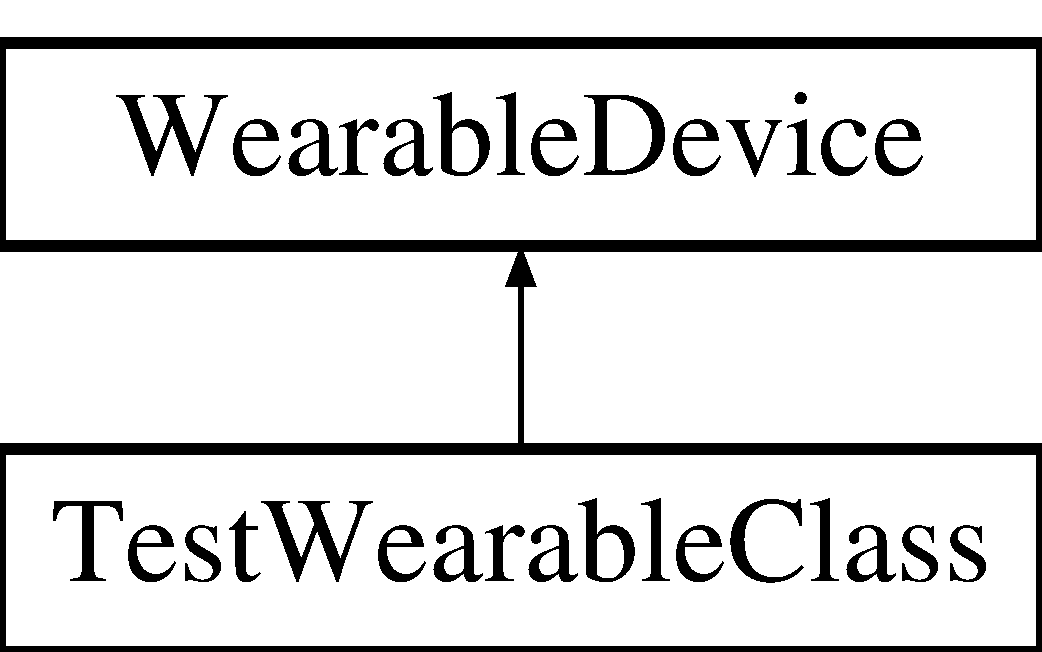
\includegraphics[height=2.000000cm]{class_test_wearable_class}
\end{center}
\end{figure}
\subsection*{Public Member Functions}
\begin{DoxyCompactItemize}
\item 
\hypertarget{class_test_wearable_class_a1d767f72a3732af62ec5a81e564dd4c4}{{\bfseries Test\+Wearable\+Class} (\hyperlink{class_shared_command_data}{Shared\+Command\+Data} $\ast$shared\+Command\+Data)}\label{class_test_wearable_class_a1d767f72a3732af62ec5a81e564dd4c4}

\item 
void \hyperlink{class_test_wearable_class_a77df79994b3f62110d884fd088388858}{run\+Device\+Loop} ()
\item 
int \hyperlink{class_test_wearable_class_ae6ba1ecadd22c18ed4ef7cf119bad740}{get\+Device\+Error} ()
\item 
\hypertarget{class_test_wearable_class_a9a3ab0cac40204faca752a9d59297b59}{bool {\bfseries is\+Done} ()}\label{class_test_wearable_class_a9a3ab0cac40204faca752a9d59297b59}

\end{DoxyCompactItemize}
\subsection*{Additional Inherited Members}


\subsection{Member Function Documentation}
\hypertarget{class_test_wearable_class_ae6ba1ecadd22c18ed4ef7cf119bad740}{\index{Test\+Wearable\+Class@{Test\+Wearable\+Class}!get\+Device\+Error@{get\+Device\+Error}}
\index{get\+Device\+Error@{get\+Device\+Error}!Test\+Wearable\+Class@{Test\+Wearable\+Class}}
\subsubsection[{get\+Device\+Error}]{\setlength{\rightskip}{0pt plus 5cm}int Test\+Wearable\+Class\+::get\+Device\+Error (
\begin{DoxyParamCaption}
{}
\end{DoxyParamCaption}
)\hspace{0.3cm}{\ttfamily [inline]}, {\ttfamily [virtual]}}}\label{class_test_wearable_class_ae6ba1ecadd22c18ed4ef7cf119bad740}
This returns a device-\/specific error code from the device, once it has stopped running. This is not necessarily thread-\/safe and should only be called once the device thread has stopped.

\begin{DoxyReturn}{Returns}
The device-\/specific error code. 
\end{DoxyReturn}


Implements \hyperlink{class_wearable_device_a1c0b4d47e9949bfcfc7111a2615538c0}{Wearable\+Device}.

\hypertarget{class_test_wearable_class_a77df79994b3f62110d884fd088388858}{\index{Test\+Wearable\+Class@{Test\+Wearable\+Class}!run\+Device\+Loop@{run\+Device\+Loop}}
\index{run\+Device\+Loop@{run\+Device\+Loop}!Test\+Wearable\+Class@{Test\+Wearable\+Class}}
\subsubsection[{run\+Device\+Loop}]{\setlength{\rightskip}{0pt plus 5cm}void Test\+Wearable\+Class\+::run\+Device\+Loop (
\begin{DoxyParamCaption}
{}
\end{DoxyParamCaption}
)\hspace{0.3cm}{\ttfamily [inline]}, {\ttfamily [virtual]}}}\label{class_test_wearable_class_a77df79994b3f62110d884fd088388858}
Runs the device loop, handling specific event handling for the device. 

Implements \hyperlink{class_wearable_device_a37bf388865b8bcf162e3fe89a23bd3e2}{Wearable\+Device}.



The documentation for this class was generated from the following file\+:\begin{DoxyCompactItemize}
\item 
Shared\+Command\+Data\+Test.\+h\end{DoxyCompactItemize}

\hypertarget{class_wearable_device}{\section{Wearable\+Device Class Reference}
\label{class_wearable_device}\index{Wearable\+Device@{Wearable\+Device}}
}


{\ttfamily \#include $<$Wearable\+Device.\+h$>$}

Inheritance diagram for Wearable\+Device\+:\begin{figure}[H]
\begin{center}
\leavevmode
\includegraphics[height=2.000000cm]{class_wearable_device}
\end{center}
\end{figure}
\subsection*{Public Member Functions}
\begin{DoxyCompactItemize}
\item 
\hypertarget{class_wearable_device_a273b604df5c2136cf7f9c114e4258366}{{\bfseries Wearable\+Device} (\hyperlink{class_shared_command_data}{Shared\+Command\+Data} $\ast$shared\+Command\+Data)}\label{class_wearable_device_a273b604df5c2136cf7f9c114e4258366}

\item 
virtual void \hyperlink{class_wearable_device_a37bf388865b8bcf162e3fe89a23bd3e2}{run\+Device\+Loop} ()=0
\item 
virtual int \hyperlink{class_wearable_device_a1c0b4d47e9949bfcfc7111a2615538c0}{get\+Device\+Error} ()=0
\item 
device\+Status \hyperlink{class_wearable_device_a118d52d7bf27041ce997feb2eac5133d}{get\+Device\+Status} ()
\item 
void \hyperlink{class_wearable_device_abcb46cb71dc666394ba20f4ed52c19f1}{stop\+Device} ()
\end{DoxyCompactItemize}
\subsection*{Protected Member Functions}
\begin{DoxyCompactItemize}
\item 
void \hyperlink{class_wearable_device_a23a9fb3a9558d9a470ef26e59599a255}{set\+Device\+Status} (device\+Status new\+Status)
\item 
bool \hyperlink{class_wearable_device_a8adbcc671888137fcc2de3298e9bf84d}{stop\+Device\+Requested} ()
\end{DoxyCompactItemize}
\subsection*{Protected Attributes}
\begin{DoxyCompactItemize}
\item 
\hypertarget{class_wearable_device_a28c355770020bcadc36655e5155ac875}{\hyperlink{class_shared_command_data}{Shared\+Command\+Data} $\ast$ {\bfseries shared\+Data}}\label{class_wearable_device_a28c355770020bcadc36655e5155ac875}

\end{DoxyCompactItemize}


\subsection{Detailed Description}
Handles a specific Midas device. 

\subsection{Member Function Documentation}
\hypertarget{class_wearable_device_a1c0b4d47e9949bfcfc7111a2615538c0}{\index{Wearable\+Device@{Wearable\+Device}!get\+Device\+Error@{get\+Device\+Error}}
\index{get\+Device\+Error@{get\+Device\+Error}!Wearable\+Device@{Wearable\+Device}}
\subsubsection[{get\+Device\+Error}]{\setlength{\rightskip}{0pt plus 5cm}virtual int Wearable\+Device\+::get\+Device\+Error (
\begin{DoxyParamCaption}
{}
\end{DoxyParamCaption}
)\hspace{0.3cm}{\ttfamily [pure virtual]}}}\label{class_wearable_device_a1c0b4d47e9949bfcfc7111a2615538c0}
This returns a device-\/specific error code from the device, once it has stopped running. This is not necessarily thread-\/safe and should only be called once the device thread has stopped.

\begin{DoxyReturn}{Returns}
The device-\/specific error code. 
\end{DoxyReturn}


Implemented in \hyperlink{class_test_wearable_class_ae6ba1ecadd22c18ed4ef7cf119bad740}{Test\+Wearable\+Class}, and \hyperlink{class_myo_device_a14db6f7115e407711091beed9b9992a6}{Myo\+Device}.

\hypertarget{class_wearable_device_a118d52d7bf27041ce997feb2eac5133d}{\index{Wearable\+Device@{Wearable\+Device}!get\+Device\+Status@{get\+Device\+Status}}
\index{get\+Device\+Status@{get\+Device\+Status}!Wearable\+Device@{Wearable\+Device}}
\subsubsection[{get\+Device\+Status}]{\setlength{\rightskip}{0pt plus 5cm}device\+Status Wearable\+Device\+::get\+Device\+Status (
\begin{DoxyParamCaption}
{}
\end{DoxyParamCaption}
)}}\label{class_wearable_device_a118d52d7bf27041ce997feb2eac5133d}
Returns the status of the device. This is thread-\/safe.

\begin{DoxyReturn}{Returns}
The status of the device. 
\end{DoxyReturn}
\hypertarget{class_wearable_device_a37bf388865b8bcf162e3fe89a23bd3e2}{\index{Wearable\+Device@{Wearable\+Device}!run\+Device\+Loop@{run\+Device\+Loop}}
\index{run\+Device\+Loop@{run\+Device\+Loop}!Wearable\+Device@{Wearable\+Device}}
\subsubsection[{run\+Device\+Loop}]{\setlength{\rightskip}{0pt plus 5cm}virtual void Wearable\+Device\+::run\+Device\+Loop (
\begin{DoxyParamCaption}
{}
\end{DoxyParamCaption}
)\hspace{0.3cm}{\ttfamily [pure virtual]}}}\label{class_wearable_device_a37bf388865b8bcf162e3fe89a23bd3e2}
Runs the device loop, handling specific event handling for the device. 

Implemented in \hyperlink{class_myo_device_a263e12e527f3984e8e2946f52d4fa111}{Myo\+Device}, and \hyperlink{class_test_wearable_class_a77df79994b3f62110d884fd088388858}{Test\+Wearable\+Class}.

\hypertarget{class_wearable_device_a23a9fb3a9558d9a470ef26e59599a255}{\index{Wearable\+Device@{Wearable\+Device}!set\+Device\+Status@{set\+Device\+Status}}
\index{set\+Device\+Status@{set\+Device\+Status}!Wearable\+Device@{Wearable\+Device}}
\subsubsection[{set\+Device\+Status}]{\setlength{\rightskip}{0pt plus 5cm}void Wearable\+Device\+::set\+Device\+Status (
\begin{DoxyParamCaption}
\item[{device\+Status}]{new\+Status}
\end{DoxyParamCaption}
)\hspace{0.3cm}{\ttfamily [protected]}}}\label{class_wearable_device_a23a9fb3a9558d9a470ef26e59599a255}
Sets the status of the device.


\begin{DoxyParams}{Parameters}
{\em new\+Status} & The new status of the device. \\
\hline
\end{DoxyParams}
\hypertarget{class_wearable_device_abcb46cb71dc666394ba20f4ed52c19f1}{\index{Wearable\+Device@{Wearable\+Device}!stop\+Device@{stop\+Device}}
\index{stop\+Device@{stop\+Device}!Wearable\+Device@{Wearable\+Device}}
\subsubsection[{stop\+Device}]{\setlength{\rightskip}{0pt plus 5cm}void Wearable\+Device\+::stop\+Device (
\begin{DoxyParamCaption}
{}
\end{DoxyParamCaption}
)}}\label{class_wearable_device_abcb46cb71dc666394ba20f4ed52c19f1}
Stops the device. This gives the device a chance to respond and perform cleanup before exiting. \hypertarget{class_wearable_device_a8adbcc671888137fcc2de3298e9bf84d}{\index{Wearable\+Device@{Wearable\+Device}!stop\+Device\+Requested@{stop\+Device\+Requested}}
\index{stop\+Device\+Requested@{stop\+Device\+Requested}!Wearable\+Device@{Wearable\+Device}}
\subsubsection[{stop\+Device\+Requested}]{\setlength{\rightskip}{0pt plus 5cm}bool Wearable\+Device\+::stop\+Device\+Requested (
\begin{DoxyParamCaption}
{}
\end{DoxyParamCaption}
)\hspace{0.3cm}{\ttfamily [protected]}}}\label{class_wearable_device_a8adbcc671888137fcc2de3298e9bf84d}
Indicates if the device has been requested to stop (by the main thread). It is the device's responsibility to check this method and, if requested to stop, perform the necessary cleanup and exit the main loop. 

The documentation for this class was generated from the following files\+:\begin{DoxyCompactItemize}
\item 
Wearable\+Device.\+h\item 
Wearable\+Device.\+cpp\end{DoxyCompactItemize}

%--- End generated contents ---

% Index
\newpage
\phantomsection
\addcontentsline{toc}{chapter}{Index}
\printindex

\end{document}
